\documentclass[twoside]{book}

% Packages required by doxygen
\usepackage{calc}
\usepackage{doxygen}
\usepackage{graphicx}
\usepackage[utf8]{inputenc}
\usepackage{makeidx}
\usepackage{multicol}
\usepackage{multirow}
\usepackage{textcomp}
\usepackage[table]{xcolor}

% Font selection
\usepackage[T1]{fontenc}
\usepackage{mathptmx}
\usepackage[scaled=.90]{helvet}
\usepackage{courier}
\usepackage{amssymb}
\usepackage{sectsty}
\renewcommand{\familydefault}{\sfdefault}
\allsectionsfont{%
  \fontseries{bc}\selectfont%
  \color{darkgray}%
}
\renewcommand{\DoxyLabelFont}{%
  \fontseries{bc}\selectfont%
  \color{darkgray}%
}

% Page & text layout
\usepackage{geometry}
\geometry{%
  a4paper,%
  top=2.5cm,%
  bottom=2.5cm,%
  left=2.5cm,%
  right=2.5cm%
}
\tolerance=750
\hfuzz=15pt
\hbadness=750
\setlength{\emergencystretch}{15pt}
\setlength{\parindent}{0cm}
\setlength{\parskip}{0.2cm}
\makeatletter
\renewcommand{\paragraph}{%
  \@startsection{paragraph}{4}{0ex}{-1.0ex}{1.0ex}{%
    \normalfont\normalsize\bfseries\SS@parafont%
  }%
}
\renewcommand{\subparagraph}{%
  \@startsection{subparagraph}{5}{0ex}{-1.0ex}{1.0ex}{%
    \normalfont\normalsize\bfseries\SS@subparafont%
  }%
}
\makeatother

% Headers & footers
\usepackage{fancyhdr}
\pagestyle{fancyplain}
\fancyhead[LE]{\fancyplain{}{\bfseries\thepage}}
\fancyhead[CE]{\fancyplain{}{}}
\fancyhead[RE]{\fancyplain{}{\bfseries\leftmark}}
\fancyhead[LO]{\fancyplain{}{\bfseries\rightmark}}
\fancyhead[CO]{\fancyplain{}{}}
\fancyhead[RO]{\fancyplain{}{\bfseries\thepage}}
\fancyfoot[LE]{\fancyplain{}{}}
\fancyfoot[CE]{\fancyplain{}{}}
\fancyfoot[RE]{\fancyplain{}{\bfseries\scriptsize Generated on Mon Mar 18 2019 22\-:09\-:39 for D\-I\-C\-E-\/friendly\-Skeletons by Doxygen }}
\fancyfoot[LO]{\fancyplain{}{\bfseries\scriptsize Generated on Mon Mar 18 2019 22\-:09\-:39 for D\-I\-C\-E-\/friendly\-Skeletons by Doxygen }}
\fancyfoot[CO]{\fancyplain{}{}}
\fancyfoot[RO]{\fancyplain{}{}}
\renewcommand{\footrulewidth}{0.4pt}
\renewcommand{\chaptermark}[1]{%
  \markboth{#1}{}%
}
\renewcommand{\sectionmark}[1]{%
  \markright{\thesection\ #1}%
}

% Indices & bibliography
\usepackage{natbib}
\usepackage[titles]{tocloft}
\setcounter{tocdepth}{3}
\setcounter{secnumdepth}{5}
\makeindex

% Hyperlinks (required, but should be loaded last)
\usepackage{ifpdf}
\ifpdf
  \usepackage[pdftex,pagebackref=true]{hyperref}
\else
  \usepackage[ps2pdf,pagebackref=true]{hyperref}
\fi
\hypersetup{%
  colorlinks=true,%
  linkcolor=blue,%
  citecolor=blue,%
  unicode%
}

% Custom commands
\newcommand{\clearemptydoublepage}{%
  \newpage{\pagestyle{empty}\cleardoublepage}%
}


%===== C O N T E N T S =====

\begin{document}

% Titlepage & ToC
\hypersetup{pageanchor=false}
\pagenumbering{roman}
\begin{titlepage}
\vspace*{7cm}
\begin{center}%
{\Large D\-I\-C\-E-\/friendly\-Skeletons }\\
\vspace*{1cm}
{\large Generated by Doxygen 1.8.5}\\
\vspace*{0.5cm}
{\small Mon Mar 18 2019 22:09:39}\\
\end{center}
\end{titlepage}
\clearemptydoublepage
\tableofcontents
\clearemptydoublepage
\pagenumbering{arabic}
\hypersetup{pageanchor=true}

%--- Begin generated contents ---
\chapter{Main Page}
\label{index}\hypertarget{index}{}\# \section*{A Parallel Skeleton Library for D\-I\-C\-E -\/ Ske\-Lib\-Ed}

\#

Descriptions of files\-:


\begin{DoxyItemize}
\item \hyperlink{def__file_8hpp}{def\-\_\-file.\-hpp} -\/$>$ Contains default definitions for the test suite.
\item \hyperlink{main_8cpp}{main.\-cpp} -\/$>$ Contain the main function.
\item \hyperlink{miscFun_8cpp}{misc\-Fun.\-cpp}/hpp -\/$>$ Contains auxilary functions for the test suite.
\item \hyperlink{test_8py}{test.\-py} -\/$>$ Contains the program that runs the test suite and plots the results.
\end{DoxyItemize}

\section*{Where S\-K\-E\-L\-E\-T\-O\-N can be \-: Map, Reduce, Map\-Reduce, Scan}


\begin{DoxyItemize}
\item test\mbox{[}-\/\-S\-K\-E\-L\-E\-T\-O\-N-\/\mbox{]}.cpp/hpp -\/$>$ Contains the simple benchmark for the S\-K\-E\-L\-E\-T\-O\-N.
\item \mbox{[}-\/\-S\-K\-E\-L\-E\-T\-O\-N-\/\mbox{]}.cpp/hpp -\/$>$ Contains the implementation of the S\-K\-E\-L\-E\-T\-O\-N.
\end{DoxyItemize}

\section*{Where P\-R\-O\-B\-L\-E\-M can be\-: Kmeans, Kmeans\-\_\-\-M\-R, \hyperlink{namespaceSummedArea}{Summed\-Area}, Radixsort}


\begin{DoxyItemize}
\item problem\mbox{[}-\/\-P\-R\-O\-B\-L\-E\-M-\/\mbox{]}.cpp/hpp -\/$>$ Contain the real-\/world problems programs. 
\end{DoxyItemize}
\chapter{Namespace Index}
\section{Namespace List}
Here is a list of all namespaces with brief descriptions\-:\begin{DoxyCompactList}
\item\contentsline{section}{\hyperlink{namespaceimpl}{impl} }{\pageref{namespaceimpl}}{}
\item\contentsline{section}{\hyperlink{namespaceKMeans}{K\-Means} }{\pageref{namespaceKMeans}}{}
\item\contentsline{section}{\hyperlink{namespaceKMeans__MapReduce}{K\-Means\-\_\-\-Map\-Reduce} }{\pageref{namespaceKMeans__MapReduce}}{}
\item\contentsline{section}{\hyperlink{namespaceRadixSort}{Radix\-Sort} }{\pageref{namespaceRadixSort}}{}
\item\contentsline{section}{\hyperlink{namespaceSummedArea}{Summed\-Area} }{\pageref{namespaceSummedArea}}{}
\item\contentsline{section}{\hyperlink{namespacetest}{test} }{\pageref{namespacetest}}{}
\end{DoxyCompactList}

\chapter{Hierarchical Index}
\section{Class Hierarchy}
This inheritance list is sorted roughly, but not completely, alphabetically\-:\begin{DoxyCompactList}
\item \contentsline{section}{K\-Means\-\_\-\-Map\-Reduce\-:\-:K\-M\-Point\-:\-:Key\-Hasher}{\pageref{structKMeans__MapReduce_1_1KMPoint_1_1KeyHasher}}{}
\item \contentsline{section}{K\-Means\-:\-:K\-M\-Point}{\pageref{structKMeans_1_1KMPoint}}{}
\item \contentsline{section}{K\-Means\-\_\-\-Map\-Reduce\-:\-:K\-M\-Point}{\pageref{classKMeans__MapReduce_1_1KMPoint}}{}
\item \contentsline{section}{Map\-Skeleton\-:\-:Map\-Implementation$<$ E\-L $>$}{\pageref{classMapSkeleton_1_1MapImplementation}}{}
\item \contentsline{section}{impl\-:\-:Map\-Overlap1\-D$<$ typename, typename, $>$}{\pageref{classimpl_1_1MapOverlap1D}}{}
\item \contentsline{section}{impl\-:\-:Map\-Overlap2\-D$<$ typename, typename, $>$}{\pageref{classimpl_1_1MapOverlap2D}}{}
\item \contentsline{section}{impl\-:\-:Map\-Overlap3\-D$<$ typename, typename, $>$}{\pageref{classimpl_1_1MapOverlap3D}}{}
\item \contentsline{section}{Map\-Reduce\-Skeleton\-:\-:Map\-Reduce\-Implementation$<$ E\-L, R\-E, H\-A $>$}{\pageref{classMapReduceSkeleton_1_1MapReduceImplementation}}{}
\item \contentsline{section}{Map\-Reduce\-Skeleton}{\pageref{classMapReduceSkeleton}}{}
\item \contentsline{section}{Map\-Skeleton}{\pageref{classMapSkeleton}}{}
\item \contentsline{section}{Pipeline}{\pageref{classPipeline}}{}
\item \contentsline{section}{Pipeline\-Init}{\pageref{classPipelineInit}}{}
\item \contentsline{section}{Pipe\-Stage\-Base}{\pageref{classPipeStageBase}}{}
\begin{DoxyCompactList}
\item \contentsline{section}{Pipe\-Stage$<$ I\-N, O\-U\-T $>$}{\pageref{classPipeStage}}{}
\item \contentsline{section}{Pipe\-Stage$<$ double, string $>$}{\pageref{classPipeStage}}{}
\begin{DoxyCompactList}
\item \contentsline{section}{Stage2}{\pageref{classStage2}}{}
\end{DoxyCompactList}
\item \contentsline{section}{Pipe\-Stage$<$ int, double $>$}{\pageref{classPipeStage}}{}
\begin{DoxyCompactList}
\item \contentsline{section}{Stage1}{\pageref{classStage1}}{}
\end{DoxyCompactList}
\item \contentsline{section}{Pipe\-Stage$<$ string, double $>$}{\pageref{classPipeStage}}{}
\begin{DoxyCompactList}
\item \contentsline{section}{Stage3}{\pageref{classStage3}}{}
\end{DoxyCompactList}
\end{DoxyCompactList}
\item \contentsline{section}{Reduce\-Skeleton\-:\-:Reduce\-Implementation$<$ C\-O $>$}{\pageref{classReduceSkeleton_1_1ReduceImplementation}}{}
\item \contentsline{section}{Reduce\-Skeleton}{\pageref{classReduceSkeleton}}{}
\item \contentsline{section}{Scan\-Skeleton\-:\-:Scan\-Implementation$<$ S\-U $>$}{\pageref{classScanSkeleton_1_1ScanImplementation}}{}
\item \contentsline{section}{Scan\-Skeleton}{\pageref{classScanSkeleton}}{}
\item \contentsline{section}{Stencil\-Skeleton\-:\-:Stencil\-Implementation$<$ E\-L $>$}{\pageref{classStencilSkeleton_1_1StencilImplementation}}{}
\item \contentsline{section}{Stencil\-Skeleton}{\pageref{classStencilSkeleton}}{}
\item \contentsline{section}{K\-Means\-:\-:Thread\-Arg\-Closest\-Centroid}{\pageref{classKMeans_1_1ThreadArgClosestCentroid}}{}
\item \contentsline{section}{Summed\-Area\-:\-:Thread\-Arg\-Get\-Area}{\pageref{classSummedArea_1_1ThreadArgGetArea}}{}
\item \contentsline{section}{Summed\-Area\-:\-:Thread\-Arg\-Get\-Summed\-Area}{\pageref{classSummedArea_1_1ThreadArgGetSummedArea}}{}
\item \contentsline{section}{K\-Means\-:\-:Thread\-Arg\-New\-Centroid}{\pageref{classKMeans_1_1ThreadArgNewCentroid}}{}
\item \contentsline{section}{K\-Means\-\_\-\-Map\-Reduce\-:\-:Thread\-Arg\-Pthread}{\pageref{classKMeans__MapReduce_1_1ThreadArgPthread}}{}
\end{DoxyCompactList}

\chapter{Class Index}
\section{Class List}
Here are the classes, structs, unions and interfaces with brief descriptions\-:\begin{DoxyCompactList}
\item\contentsline{section}{\hyperlink{structKMeans__MapReduce_1_1KMPoint_1_1KeyHasher}{K\-Means\-\_\-\-Map\-Reduce\-::\-K\-M\-Point\-::\-Key\-Hasher} }{\pageref{structKMeans__MapReduce_1_1KMPoint_1_1KeyHasher}}{}
\item\contentsline{section}{\hyperlink{structKMeans_1_1KMPoint}{K\-Means\-::\-K\-M\-Point} }{\pageref{structKMeans_1_1KMPoint}}{}
\item\contentsline{section}{\hyperlink{classKMeans__MapReduce_1_1KMPoint}{K\-Means\-\_\-\-Map\-Reduce\-::\-K\-M\-Point} }{\pageref{classKMeans__MapReduce_1_1KMPoint}}{}
\item\contentsline{section}{\hyperlink{classMapSkeleton_1_1MapImplementation}{Map\-Skeleton\-::\-Map\-Implementation$<$ E\-L $>$} }{\pageref{classMapSkeleton_1_1MapImplementation}}{}
\item\contentsline{section}{\hyperlink{classimpl_1_1MapOverlap1D}{impl\-::\-Map\-Overlap1\-D$<$ typename, typename, $>$} }{\pageref{classimpl_1_1MapOverlap1D}}{}
\item\contentsline{section}{\hyperlink{classimpl_1_1MapOverlap2D}{impl\-::\-Map\-Overlap2\-D$<$ typename, typename, $>$} }{\pageref{classimpl_1_1MapOverlap2D}}{}
\item\contentsline{section}{\hyperlink{classimpl_1_1MapOverlap3D}{impl\-::\-Map\-Overlap3\-D$<$ typename, typename, $>$} }{\pageref{classimpl_1_1MapOverlap3D}}{}
\item\contentsline{section}{\hyperlink{classMapReduceSkeleton_1_1MapReduceImplementation}{Map\-Reduce\-Skeleton\-::\-Map\-Reduce\-Implementation$<$ E\-L, R\-E, H\-A $>$} }{\pageref{classMapReduceSkeleton_1_1MapReduceImplementation}}{}
\item\contentsline{section}{\hyperlink{classMapReduceSkeleton}{Map\-Reduce\-Skeleton} }{\pageref{classMapReduceSkeleton}}{}
\item\contentsline{section}{\hyperlink{classMapSkeleton}{Map\-Skeleton} }{\pageref{classMapSkeleton}}{}
\item\contentsline{section}{\hyperlink{classPipeline}{Pipeline} }{\pageref{classPipeline}}{}
\item\contentsline{section}{\hyperlink{classPipelineInit}{Pipeline\-Init} }{\pageref{classPipelineInit}}{}
\item\contentsline{section}{\hyperlink{classPipeStage}{Pipe\-Stage$<$ I\-N, O\-U\-T $>$} }{\pageref{classPipeStage}}{}
\item\contentsline{section}{\hyperlink{classPipeStageBase}{Pipe\-Stage\-Base} }{\pageref{classPipeStageBase}}{}
\item\contentsline{section}{\hyperlink{classReduceSkeleton_1_1ReduceImplementation}{Reduce\-Skeleton\-::\-Reduce\-Implementation$<$ C\-O $>$} }{\pageref{classReduceSkeleton_1_1ReduceImplementation}}{}
\item\contentsline{section}{\hyperlink{classReduceSkeleton}{Reduce\-Skeleton} }{\pageref{classReduceSkeleton}}{}
\item\contentsline{section}{\hyperlink{classScanSkeleton_1_1ScanImplementation}{Scan\-Skeleton\-::\-Scan\-Implementation$<$ S\-U $>$} }{\pageref{classScanSkeleton_1_1ScanImplementation}}{}
\item\contentsline{section}{\hyperlink{classScanSkeleton}{Scan\-Skeleton} }{\pageref{classScanSkeleton}}{}
\item\contentsline{section}{\hyperlink{classStage1}{Stage1} }{\pageref{classStage1}}{}
\item\contentsline{section}{\hyperlink{classStage2}{Stage2} }{\pageref{classStage2}}{}
\item\contentsline{section}{\hyperlink{classStage3}{Stage3} }{\pageref{classStage3}}{}
\item\contentsline{section}{\hyperlink{classStencilSkeleton_1_1StencilImplementation}{Stencil\-Skeleton\-::\-Stencil\-Implementation$<$ E\-L $>$} }{\pageref{classStencilSkeleton_1_1StencilImplementation}}{}
\item\contentsline{section}{\hyperlink{classStencilSkeleton}{Stencil\-Skeleton} }{\pageref{classStencilSkeleton}}{}
\item\contentsline{section}{\hyperlink{classKMeans_1_1ThreadArgClosestCentroid}{K\-Means\-::\-Thread\-Arg\-Closest\-Centroid} }{\pageref{classKMeans_1_1ThreadArgClosestCentroid}}{}
\item\contentsline{section}{\hyperlink{classSummedArea_1_1ThreadArgGetArea}{Summed\-Area\-::\-Thread\-Arg\-Get\-Area} }{\pageref{classSummedArea_1_1ThreadArgGetArea}}{}
\item\contentsline{section}{\hyperlink{classSummedArea_1_1ThreadArgGetSummedArea}{Summed\-Area\-::\-Thread\-Arg\-Get\-Summed\-Area} }{\pageref{classSummedArea_1_1ThreadArgGetSummedArea}}{}
\item\contentsline{section}{\hyperlink{classKMeans_1_1ThreadArgNewCentroid}{K\-Means\-::\-Thread\-Arg\-New\-Centroid} }{\pageref{classKMeans_1_1ThreadArgNewCentroid}}{}
\item\contentsline{section}{\hyperlink{classKMeans__MapReduce_1_1ThreadArgPthread}{K\-Means\-\_\-\-Map\-Reduce\-::\-Thread\-Arg\-Pthread} }{\pageref{classKMeans__MapReduce_1_1ThreadArgPthread}}{}
\end{DoxyCompactList}

\chapter{File Index}
\section{File List}
Here is a list of all files with brief descriptions\-:\begin{DoxyCompactList}
\item\contentsline{section}{Distribute/\hyperlink{Stencil_8hpp}{Stencil.\-hpp} }{\pageref{Stencil_8hpp}}{}
\end{DoxyCompactList}

\chapter{Namespace Documentation}
\hypertarget{namespaceimpl}{\section{impl Namespace Reference}
\label{namespaceimpl}\index{impl@{impl}}
}
\subsection*{Classes}
\begin{DoxyCompactItemize}
\item 
class \hyperlink{classimpl_1_1MapOverlap1D}{Map\-Overlap1\-D}
\item 
class \hyperlink{classimpl_1_1MapOverlap2D}{Map\-Overlap2\-D}
\item 
class \hyperlink{classimpl_1_1MapOverlap3D}{Map\-Overlap3\-D}
\end{DoxyCompactItemize}

\hypertarget{namespaceKMeans}{\section{K\-Means Namespace Reference}
\label{namespaceKMeans}\index{K\-Means@{K\-Means}}
}
\subsection*{Classes}
\begin{DoxyCompactItemize}
\item 
struct \hyperlink{structKMeans_1_1KMPoint}{K\-M\-Point}
\item 
class \hyperlink{classKMeans_1_1ThreadArgClosestCentroid}{Thread\-Arg\-Closest\-Centroid}
\item 
class \hyperlink{classKMeans_1_1ThreadArgNewCentroid}{Thread\-Arg\-New\-Centroid}
\end{DoxyCompactItemize}
\subsection*{Typedefs}
\begin{DoxyCompactItemize}
\item 
typedef std\-::pair$<$ double, double $>$ \hyperlink{namespaceKMeans_a32ce08f4c8b30171faaeff5a3a466f30}{C\-O\-O\-R\-D}
\end{DoxyCompactItemize}
\subsection*{Functions}
\begin{DoxyCompactItemize}
\item 
int \hyperlink{namespaceKMeans_aeccf7b9a20677968be2392b189462968}{i\-Rand} (int i\-Min, int i\-Max)
\item 
double \hyperlink{namespaceKMeans_aa1cc53313a5e71901410db444f2f1277}{f\-Rand} (double f\-Min=0.\-0, double f\-Max=1.\-0)
\item 
double \hyperlink{namespaceKMeans_ab1d0698be0b64e379858f444df37f184}{distance\-Of} (\hyperlink{namespaceKMeans_a32ce08f4c8b30171faaeff5a3a466f30}{C\-O\-O\-R\-D} \&p1, \hyperlink{namespaceKMeans_a32ce08f4c8b30171faaeff5a3a466f30}{C\-O\-O\-R\-D} \&p2)
\item 
\hyperlink{structKMeans_1_1KMPoint}{K\-M\-Point} $\ast$ \hyperlink{namespaceKMeans_a1290694d35842d45c40524d6f1d4cc01}{elemental} (\hyperlink{structKMeans_1_1KMPoint}{K\-M\-Point} $\ast$point, std\-::vector$<$ \hyperlink{structKMeans_1_1KMPoint}{K\-M\-Point} $>$ \&centroids)
\item 
{\footnotesize template$<$typename R $>$ }\\\hyperlink{structKMeans_1_1KMPoint}{K\-M\-Point} \hyperlink{namespaceKMeans_af6ddf3d8fcb489e1b35093fe7387a135}{map\-To\-New\-Centroid\-Elemental} (std\-::vector$<$ \hyperlink{structKMeans_1_1KMPoint}{K\-M\-Point} $\ast$ $>$ $\ast$points\-In\-Centroid, R \&reduce)
\item 
\hyperlink{structKMeans_1_1KMPoint}{K\-M\-Point} $\ast$ \hyperlink{namespaceKMeans_a59f0fc44e94dd722fea19b2c130b7811}{combiner} (\hyperlink{structKMeans_1_1KMPoint}{K\-M\-Point} $\ast$p1, \hyperlink{structKMeans_1_1KMPoint}{K\-M\-Point} $\ast$p2)
\item 
void \hyperlink{namespaceKMeans_a0168f204720c7b64714f53f142004a36}{print\-K\-M\-Point} (\hyperlink{structKMeans_1_1KMPoint}{K\-M\-Point} point)
\item 
std\-::vector$<$ \hyperlink{structKMeans_1_1KMPoint}{K\-M\-Point} $>$ \hyperlink{namespaceKMeans_a2aadc9387de95e9488dd5605465f7cd1}{K\-Means\-Skel} (std\-::vector$<$ \hyperlink{structKMeans_1_1KMPoint}{K\-M\-Point} $>$ points, std\-::vector$<$ \hyperlink{structKMeans_1_1KMPoint}{K\-M\-Point} $>$ centroids, std\-::vector$<$ double $>$ \&map\-Timings, std\-::vector$<$ double $>$ \&reduce\-Timings, std\-::vector$<$ double $>$ \&skel\-Seq\-Timing)
\item 
void \hyperlink{namespaceKMeans_a51a34cb9e3c9fa1b619342ce80834c7b}{seq\-Find\-Closest\-Centroid} (std\-::vector$<$ \hyperlink{structKMeans_1_1KMPoint}{K\-M\-Point} $\ast$ $>$ \&points, std\-::vector$<$ \hyperlink{structKMeans_1_1KMPoint}{K\-M\-Point} $>$ \&centroids)
\item 
void \hyperlink{namespaceKMeans_a3be77d9de58b3e3151ceb2a48681d40f}{seq\-Find\-New\-Centroids} (\hyperlink{structKMeans_1_1KMPoint}{K\-M\-Point} \&new\-Centroid, std\-::vector$<$ \hyperlink{structKMeans_1_1KMPoint}{K\-M\-Point} $\ast$ $>$ \&points)
\item 
std\-::vector$<$ \hyperlink{structKMeans_1_1KMPoint}{K\-M\-Point} $>$ \hyperlink{namespaceKMeans_a10702545b2f1319336b2789ee42e1bd6}{K\-Means\-Seq} (std\-::vector$<$ \hyperlink{structKMeans_1_1KMPoint}{K\-M\-Point} $>$ points, std\-::vector$<$ \hyperlink{structKMeans_1_1KMPoint}{K\-M\-Point} $>$ centroids, std\-::vector$<$ double $>$ \&non\-Parallel\-Timings)
\item 
void \hyperlink{namespaceKMeans_af1d43ce3d20a17d12527e0fac7832f37}{pthread\-Closest\-Centroid} (\hyperlink{classKMeans_1_1ThreadArgClosestCentroid}{Thread\-Arg\-Closest\-Centroid} $\ast$thread\-Arguments, size\-\_\-t thread\-I\-D)
\item 
void \hyperlink{namespaceKMeans_a760600cbd27b19e04a612fa75b2e3d3b}{pthread\-New\-Centroid\-Barrier} (size\-\_\-t n\-Threads\-To\-Barrier)
\item 
void \hyperlink{namespaceKMeans_a7bbfb7d54cedb05d039f1660792b007d}{pthread\-New\-Centroid} (std\-::vector$<$ \hyperlink{classKMeans_1_1ThreadArgNewCentroid}{Thread\-Arg\-New\-Centroid} $>$ $\ast$thread\-Arguments, size\-\_\-t thread\-I\-D)
\item 
void \hyperlink{namespaceKMeans_abf69c32edce6417d0dce98e983c35af4}{p\-Threads\-Find\-New\-Centroid} (\hyperlink{structKMeans_1_1KMPoint}{K\-M\-Point} \&new\-Centroid, std\-::vector$<$ \hyperlink{structKMeans_1_1KMPoint}{K\-M\-Point} $\ast$ $>$ \&points)
\item 
std\-::vector$<$ \hyperlink{structKMeans_1_1KMPoint}{K\-M\-Point} $>$ \hyperlink{namespaceKMeans_a37946d061f5cdb3de7465fb0dca1a16e}{K\-Means\-P\-Threads} (std\-::vector$<$ \hyperlink{structKMeans_1_1KMPoint}{K\-M\-Point} $>$ points, std\-::vector$<$ \hyperlink{structKMeans_1_1KMPoint}{K\-M\-Point} $>$ centroids, std\-::vector$<$ double $>$ \&non\-Parallel\-Timings)
\item 
int \hyperlink{namespaceKMeans_ab6f8f31e6f0f753d15f544e340cf44d9}{K\-Means\-Main} (int argc, char $\ast$$\ast$argv)
\end{DoxyCompactItemize}
\subsection*{Variables}
\begin{DoxyCompactItemize}
\item 
std\-::mutex \hyperlink{namespaceKMeans_a5219c2c9759a95b517b455049f6563de}{pthread\-Barrier\-Lock}
\item 
std\-::condition\-\_\-variable \hyperlink{namespaceKMeans_a1001aa3caa40eaebdd2d3d500f313348}{pthread\-Cond\-\_\-\-Var}
\item 
size\-\_\-t \hyperlink{namespaceKMeans_ad847e407438dfefa275c4be95c2b46ef}{pthread\-Threads\-Arrived}
\end{DoxyCompactItemize}


\subsection{Typedef Documentation}
\hypertarget{namespaceKMeans_a32ce08f4c8b30171faaeff5a3a466f30}{\index{K\-Means@{K\-Means}!C\-O\-O\-R\-D@{C\-O\-O\-R\-D}}
\index{C\-O\-O\-R\-D@{C\-O\-O\-R\-D}!KMeans@{K\-Means}}
\subsubsection[{C\-O\-O\-R\-D}]{\setlength{\rightskip}{0pt plus 5cm}typedef std\-::pair$<$double, double$>$ {\bf K\-Means\-::\-C\-O\-O\-R\-D}}}\label{namespaceKMeans_a32ce08f4c8b30171faaeff5a3a466f30}


\subsection{Function Documentation}
\hypertarget{namespaceKMeans_a59f0fc44e94dd722fea19b2c130b7811}{\index{K\-Means@{K\-Means}!combiner@{combiner}}
\index{combiner@{combiner}!KMeans@{K\-Means}}
\subsubsection[{combiner}]{\setlength{\rightskip}{0pt plus 5cm}{\bf K\-M\-Point}$\ast$ K\-Means\-::combiner (
\begin{DoxyParamCaption}
\item[{K\-M\-Point $\ast$}]{p1, }
\item[{K\-M\-Point $\ast$}]{p2}
\end{DoxyParamCaption}
)}}\label{namespaceKMeans_a59f0fc44e94dd722fea19b2c130b7811}
\hypertarget{namespaceKMeans_ab1d0698be0b64e379858f444df37f184}{\index{K\-Means@{K\-Means}!distance\-Of@{distance\-Of}}
\index{distance\-Of@{distance\-Of}!KMeans@{K\-Means}}
\subsubsection[{distance\-Of}]{\setlength{\rightskip}{0pt plus 5cm}double K\-Means\-::distance\-Of (
\begin{DoxyParamCaption}
\item[{C\-O\-O\-R\-D \&}]{p1, }
\item[{C\-O\-O\-R\-D \&}]{p2}
\end{DoxyParamCaption}
)}}\label{namespaceKMeans_ab1d0698be0b64e379858f444df37f184}
\hypertarget{namespaceKMeans_a1290694d35842d45c40524d6f1d4cc01}{\index{K\-Means@{K\-Means}!elemental@{elemental}}
\index{elemental@{elemental}!KMeans@{K\-Means}}
\subsubsection[{elemental}]{\setlength{\rightskip}{0pt plus 5cm}{\bf K\-M\-Point}$\ast$ K\-Means\-::elemental (
\begin{DoxyParamCaption}
\item[{K\-M\-Point $\ast$}]{point, }
\item[{std\-::vector$<$ K\-M\-Point $>$ \&}]{centroids}
\end{DoxyParamCaption}
)}}\label{namespaceKMeans_a1290694d35842d45c40524d6f1d4cc01}
\hypertarget{namespaceKMeans_aa1cc53313a5e71901410db444f2f1277}{\index{K\-Means@{K\-Means}!f\-Rand@{f\-Rand}}
\index{f\-Rand@{f\-Rand}!KMeans@{K\-Means}}
\subsubsection[{f\-Rand}]{\setlength{\rightskip}{0pt plus 5cm}double K\-Means\-::f\-Rand (
\begin{DoxyParamCaption}
\item[{double}]{f\-Min = {\ttfamily 0.0}, }
\item[{double}]{f\-Max = {\ttfamily 1.0}}
\end{DoxyParamCaption}
)}}\label{namespaceKMeans_aa1cc53313a5e71901410db444f2f1277}
\hypertarget{namespaceKMeans_aeccf7b9a20677968be2392b189462968}{\index{K\-Means@{K\-Means}!i\-Rand@{i\-Rand}}
\index{i\-Rand@{i\-Rand}!KMeans@{K\-Means}}
\subsubsection[{i\-Rand}]{\setlength{\rightskip}{0pt plus 5cm}int K\-Means\-::i\-Rand (
\begin{DoxyParamCaption}
\item[{int}]{i\-Min, }
\item[{int}]{i\-Max}
\end{DoxyParamCaption}
)}}\label{namespaceKMeans_aeccf7b9a20677968be2392b189462968}
\hypertarget{namespaceKMeans_ab6f8f31e6f0f753d15f544e340cf44d9}{\index{K\-Means@{K\-Means}!K\-Means\-Main@{K\-Means\-Main}}
\index{K\-Means\-Main@{K\-Means\-Main}!KMeans@{K\-Means}}
\subsubsection[{K\-Means\-Main}]{\setlength{\rightskip}{0pt plus 5cm}int K\-Means\-::\-K\-Means\-Main (
\begin{DoxyParamCaption}
\item[{int}]{argc, }
\item[{char $\ast$$\ast$}]{argv}
\end{DoxyParamCaption}
)}}\label{namespaceKMeans_ab6f8f31e6f0f753d15f544e340cf44d9}
\hypertarget{namespaceKMeans_a37946d061f5cdb3de7465fb0dca1a16e}{\index{K\-Means@{K\-Means}!K\-Means\-P\-Threads@{K\-Means\-P\-Threads}}
\index{K\-Means\-P\-Threads@{K\-Means\-P\-Threads}!KMeans@{K\-Means}}
\subsubsection[{K\-Means\-P\-Threads}]{\setlength{\rightskip}{0pt plus 5cm}std\-::vector$<${\bf K\-M\-Point}$>$ K\-Means\-::\-K\-Means\-P\-Threads (
\begin{DoxyParamCaption}
\item[{std\-::vector$<$ K\-M\-Point $>$}]{points, }
\item[{std\-::vector$<$ K\-M\-Point $>$}]{centroids, }
\item[{std\-::vector$<$ double $>$ \&}]{non\-Parallel\-Timings}
\end{DoxyParamCaption}
)}}\label{namespaceKMeans_a37946d061f5cdb3de7465fb0dca1a16e}
\hypertarget{namespaceKMeans_a10702545b2f1319336b2789ee42e1bd6}{\index{K\-Means@{K\-Means}!K\-Means\-Seq@{K\-Means\-Seq}}
\index{K\-Means\-Seq@{K\-Means\-Seq}!KMeans@{K\-Means}}
\subsubsection[{K\-Means\-Seq}]{\setlength{\rightskip}{0pt plus 5cm}std\-::vector$<${\bf K\-M\-Point}$>$ K\-Means\-::\-K\-Means\-Seq (
\begin{DoxyParamCaption}
\item[{std\-::vector$<$ K\-M\-Point $>$}]{points, }
\item[{std\-::vector$<$ K\-M\-Point $>$}]{centroids, }
\item[{std\-::vector$<$ double $>$ \&}]{non\-Parallel\-Timings}
\end{DoxyParamCaption}
)}}\label{namespaceKMeans_a10702545b2f1319336b2789ee42e1bd6}
\hypertarget{namespaceKMeans_a2aadc9387de95e9488dd5605465f7cd1}{\index{K\-Means@{K\-Means}!K\-Means\-Skel@{K\-Means\-Skel}}
\index{K\-Means\-Skel@{K\-Means\-Skel}!KMeans@{K\-Means}}
\subsubsection[{K\-Means\-Skel}]{\setlength{\rightskip}{0pt plus 5cm}std\-::vector$<${\bf K\-M\-Point}$>$ K\-Means\-::\-K\-Means\-Skel (
\begin{DoxyParamCaption}
\item[{std\-::vector$<$ K\-M\-Point $>$}]{points, }
\item[{std\-::vector$<$ K\-M\-Point $>$}]{centroids, }
\item[{std\-::vector$<$ double $>$ \&}]{map\-Timings, }
\item[{std\-::vector$<$ double $>$ \&}]{reduce\-Timings, }
\item[{std\-::vector$<$ double $>$ \&}]{skel\-Seq\-Timing}
\end{DoxyParamCaption}
)}}\label{namespaceKMeans_a2aadc9387de95e9488dd5605465f7cd1}
\hypertarget{namespaceKMeans_af6ddf3d8fcb489e1b35093fe7387a135}{\index{K\-Means@{K\-Means}!map\-To\-New\-Centroid\-Elemental@{map\-To\-New\-Centroid\-Elemental}}
\index{map\-To\-New\-Centroid\-Elemental@{map\-To\-New\-Centroid\-Elemental}!KMeans@{K\-Means}}
\subsubsection[{map\-To\-New\-Centroid\-Elemental}]{\setlength{\rightskip}{0pt plus 5cm}template$<$typename R $>$ {\bf K\-M\-Point} K\-Means\-::map\-To\-New\-Centroid\-Elemental (
\begin{DoxyParamCaption}
\item[{std\-::vector$<$ K\-M\-Point $\ast$ $>$ $\ast$}]{points\-In\-Centroid, }
\item[{R \&}]{reduce}
\end{DoxyParamCaption}
)}}\label{namespaceKMeans_af6ddf3d8fcb489e1b35093fe7387a135}
\hypertarget{namespaceKMeans_a0168f204720c7b64714f53f142004a36}{\index{K\-Means@{K\-Means}!print\-K\-M\-Point@{print\-K\-M\-Point}}
\index{print\-K\-M\-Point@{print\-K\-M\-Point}!KMeans@{K\-Means}}
\subsubsection[{print\-K\-M\-Point}]{\setlength{\rightskip}{0pt plus 5cm}void K\-Means\-::print\-K\-M\-Point (
\begin{DoxyParamCaption}
\item[{K\-M\-Point}]{point}
\end{DoxyParamCaption}
)}}\label{namespaceKMeans_a0168f204720c7b64714f53f142004a36}
\hypertarget{namespaceKMeans_af1d43ce3d20a17d12527e0fac7832f37}{\index{K\-Means@{K\-Means}!pthread\-Closest\-Centroid@{pthread\-Closest\-Centroid}}
\index{pthread\-Closest\-Centroid@{pthread\-Closest\-Centroid}!KMeans@{K\-Means}}
\subsubsection[{pthread\-Closest\-Centroid}]{\setlength{\rightskip}{0pt plus 5cm}void K\-Means\-::pthread\-Closest\-Centroid (
\begin{DoxyParamCaption}
\item[{Thread\-Arg\-Closest\-Centroid $\ast$}]{thread\-Arguments, }
\item[{size\-\_\-t}]{thread\-I\-D}
\end{DoxyParamCaption}
)}}\label{namespaceKMeans_af1d43ce3d20a17d12527e0fac7832f37}
\hypertarget{namespaceKMeans_a7bbfb7d54cedb05d039f1660792b007d}{\index{K\-Means@{K\-Means}!pthread\-New\-Centroid@{pthread\-New\-Centroid}}
\index{pthread\-New\-Centroid@{pthread\-New\-Centroid}!KMeans@{K\-Means}}
\subsubsection[{pthread\-New\-Centroid}]{\setlength{\rightskip}{0pt plus 5cm}void K\-Means\-::pthread\-New\-Centroid (
\begin{DoxyParamCaption}
\item[{std\-::vector$<$ Thread\-Arg\-New\-Centroid $>$ $\ast$}]{thread\-Arguments, }
\item[{size\-\_\-t}]{thread\-I\-D}
\end{DoxyParamCaption}
)}}\label{namespaceKMeans_a7bbfb7d54cedb05d039f1660792b007d}
\hypertarget{namespaceKMeans_a760600cbd27b19e04a612fa75b2e3d3b}{\index{K\-Means@{K\-Means}!pthread\-New\-Centroid\-Barrier@{pthread\-New\-Centroid\-Barrier}}
\index{pthread\-New\-Centroid\-Barrier@{pthread\-New\-Centroid\-Barrier}!KMeans@{K\-Means}}
\subsubsection[{pthread\-New\-Centroid\-Barrier}]{\setlength{\rightskip}{0pt plus 5cm}void K\-Means\-::pthread\-New\-Centroid\-Barrier (
\begin{DoxyParamCaption}
\item[{size\-\_\-t}]{n\-Threads\-To\-Barrier}
\end{DoxyParamCaption}
)}}\label{namespaceKMeans_a760600cbd27b19e04a612fa75b2e3d3b}
\hypertarget{namespaceKMeans_abf69c32edce6417d0dce98e983c35af4}{\index{K\-Means@{K\-Means}!p\-Threads\-Find\-New\-Centroid@{p\-Threads\-Find\-New\-Centroid}}
\index{p\-Threads\-Find\-New\-Centroid@{p\-Threads\-Find\-New\-Centroid}!KMeans@{K\-Means}}
\subsubsection[{p\-Threads\-Find\-New\-Centroid}]{\setlength{\rightskip}{0pt plus 5cm}void K\-Means\-::p\-Threads\-Find\-New\-Centroid (
\begin{DoxyParamCaption}
\item[{K\-M\-Point \&}]{new\-Centroid, }
\item[{std\-::vector$<$ K\-M\-Point $\ast$ $>$ \&}]{points}
\end{DoxyParamCaption}
)}}\label{namespaceKMeans_abf69c32edce6417d0dce98e983c35af4}
\hypertarget{namespaceKMeans_a51a34cb9e3c9fa1b619342ce80834c7b}{\index{K\-Means@{K\-Means}!seq\-Find\-Closest\-Centroid@{seq\-Find\-Closest\-Centroid}}
\index{seq\-Find\-Closest\-Centroid@{seq\-Find\-Closest\-Centroid}!KMeans@{K\-Means}}
\subsubsection[{seq\-Find\-Closest\-Centroid}]{\setlength{\rightskip}{0pt plus 5cm}void K\-Means\-::seq\-Find\-Closest\-Centroid (
\begin{DoxyParamCaption}
\item[{std\-::vector$<$ K\-M\-Point $\ast$ $>$ \&}]{points, }
\item[{std\-::vector$<$ K\-M\-Point $>$ \&}]{centroids}
\end{DoxyParamCaption}
)}}\label{namespaceKMeans_a51a34cb9e3c9fa1b619342ce80834c7b}
\hypertarget{namespaceKMeans_a3be77d9de58b3e3151ceb2a48681d40f}{\index{K\-Means@{K\-Means}!seq\-Find\-New\-Centroids@{seq\-Find\-New\-Centroids}}
\index{seq\-Find\-New\-Centroids@{seq\-Find\-New\-Centroids}!KMeans@{K\-Means}}
\subsubsection[{seq\-Find\-New\-Centroids}]{\setlength{\rightskip}{0pt plus 5cm}void K\-Means\-::seq\-Find\-New\-Centroids (
\begin{DoxyParamCaption}
\item[{K\-M\-Point \&}]{new\-Centroid, }
\item[{std\-::vector$<$ K\-M\-Point $\ast$ $>$ \&}]{points}
\end{DoxyParamCaption}
)}}\label{namespaceKMeans_a3be77d9de58b3e3151ceb2a48681d40f}


\subsection{Variable Documentation}
\hypertarget{namespaceKMeans_a5219c2c9759a95b517b455049f6563de}{\index{K\-Means@{K\-Means}!pthread\-Barrier\-Lock@{pthread\-Barrier\-Lock}}
\index{pthread\-Barrier\-Lock@{pthread\-Barrier\-Lock}!KMeans@{K\-Means}}
\subsubsection[{pthread\-Barrier\-Lock}]{\setlength{\rightskip}{0pt plus 5cm}std\-::mutex K\-Means\-::pthread\-Barrier\-Lock}}\label{namespaceKMeans_a5219c2c9759a95b517b455049f6563de}
\hypertarget{namespaceKMeans_a1001aa3caa40eaebdd2d3d500f313348}{\index{K\-Means@{K\-Means}!pthread\-Cond\-\_\-\-Var@{pthread\-Cond\-\_\-\-Var}}
\index{pthread\-Cond\-\_\-\-Var@{pthread\-Cond\-\_\-\-Var}!KMeans@{K\-Means}}
\subsubsection[{pthread\-Cond\-\_\-\-Var}]{\setlength{\rightskip}{0pt plus 5cm}std\-::condition\-\_\-variable K\-Means\-::pthread\-Cond\-\_\-\-Var}}\label{namespaceKMeans_a1001aa3caa40eaebdd2d3d500f313348}
\hypertarget{namespaceKMeans_ad847e407438dfefa275c4be95c2b46ef}{\index{K\-Means@{K\-Means}!pthread\-Threads\-Arrived@{pthread\-Threads\-Arrived}}
\index{pthread\-Threads\-Arrived@{pthread\-Threads\-Arrived}!KMeans@{K\-Means}}
\subsubsection[{pthread\-Threads\-Arrived}]{\setlength{\rightskip}{0pt plus 5cm}size\-\_\-t K\-Means\-::pthread\-Threads\-Arrived}}\label{namespaceKMeans_ad847e407438dfefa275c4be95c2b46ef}

\hypertarget{namespaceKMeans__MapReduce}{\section{K\-Means\-\_\-\-Map\-Reduce Namespace Reference}
\label{namespaceKMeans__MapReduce}\index{K\-Means\-\_\-\-Map\-Reduce@{K\-Means\-\_\-\-Map\-Reduce}}
}
\subsection*{Classes}
\begin{DoxyCompactItemize}
\item 
class \hyperlink{classKMeans__MapReduce_1_1KMPoint}{K\-M\-Point}
\item 
class \hyperlink{classKMeans__MapReduce_1_1ThreadArgPthread}{Thread\-Arg\-Pthread}
\end{DoxyCompactItemize}
\subsection*{Typedefs}
\begin{DoxyCompactItemize}
\item 
typedef std\-::pair$<$ double, double $>$ \hyperlink{namespaceKMeans__MapReduce_a8dfbbc4a186c8ea8ae691f4a85db53e3}{C\-O\-O\-R\-D}
\end{DoxyCompactItemize}
\subsection*{Functions}
\begin{DoxyCompactItemize}
\item 
int \hyperlink{namespaceKMeans__MapReduce_afdd814de48bd8f8ee4d3b5046452e120}{i\-Rand} (int i\-Min, int i\-Max)
\item 
double \hyperlink{namespaceKMeans__MapReduce_add51d8d3039809f3398107c0875c8c1b}{f\-Rand} (double f\-Min=0.\-0, double f\-Max=1.\-0)
\item 
double \hyperlink{namespaceKMeans__MapReduce_a641fcf6cec59b7626e10e89a580b3d3d}{distance\-Of} (\hyperlink{namespaceKMeans__MapReduce_a8dfbbc4a186c8ea8ae691f4a85db53e3}{C\-O\-O\-R\-D} \&p1, \hyperlink{namespaceKMeans__MapReduce_a8dfbbc4a186c8ea8ae691f4a85db53e3}{C\-O\-O\-R\-D} \&p2)
\item 
void \hyperlink{namespaceKMeans__MapReduce_a7cb6ca49c0fa1c2277452c37bccf53e1}{print\-K\-M\-Point} (\hyperlink{classKMeans__MapReduce_1_1KMPoint}{K\-M\-Point} point)
\item 
std\-::list$<$ std\-::pair$<$ \hyperlink{classKMeans__MapReduce_1_1KMPoint}{K\-M\-Point}, \\*
\hyperlink{classKMeans__MapReduce_1_1KMPoint}{K\-M\-Point} $>$ $>$ \hyperlink{namespaceKMeans__MapReduce_a2c7d89ec14b9139bef11124ced4b6379}{elemental\-M\-R\-\_\-\-Get\-Closest\-Centroid} (\hyperlink{classKMeans__MapReduce_1_1KMPoint}{K\-M\-Point} point, std\-::vector$<$ \hyperlink{classKMeans__MapReduce_1_1KMPoint}{K\-M\-Point} $>$ \&centroids)
\item 
std\-::list$<$ \hyperlink{classKMeans__MapReduce_1_1KMPoint}{K\-M\-Point} $>$ \hyperlink{namespaceKMeans__MapReduce_a0c17f1e970fe25155d1019441692f230}{combiner\-M\-R\-\_\-\-Get\-New\-Centroid} (\hyperlink{classKMeans__MapReduce_1_1KMPoint}{K\-M\-Point} \&centroid, std\-::list$<$ \hyperlink{classKMeans__MapReduce_1_1KMPoint}{K\-M\-Point} $>$ points, std\-::vector$<$ \hyperlink{classKMeans__MapReduce_1_1KMPoint}{K\-M\-Point} $>$)
\item 
std\-::vector$<$ \hyperlink{classKMeans__MapReduce_1_1KMPoint}{K\-M\-Point} $>$ \hyperlink{namespaceKMeans__MapReduce_a2ecd357b5ea731ac0ca5b12f64ab9326}{K\-Means\-M\-R\-\_\-\-Skel} (std\-::vector$<$ \hyperlink{classKMeans__MapReduce_1_1KMPoint}{K\-M\-Point} $>$ points, std\-::vector$<$ \hyperlink{classKMeans__MapReduce_1_1KMPoint}{K\-M\-Point} $>$ centroids, std\-::vector$<$ double $>$ \&map\-Reduce\-Timings, std\-::vector$<$ double $>$ \&skel\-Seq\-Timing)
\item 
std\-::vector$<$ \hyperlink{classKMeans__MapReduce_1_1KMPoint}{K\-M\-Point} $>$ \hyperlink{namespaceKMeans__MapReduce_ab76faaf9ab0206e28cb35c0860b219b1}{K\-Means\-M\-R\-\_\-\-Seq} (std\-::vector$<$ \hyperlink{classKMeans__MapReduce_1_1KMPoint}{K\-M\-Point} $>$ points, std\-::vector$<$ \hyperlink{classKMeans__MapReduce_1_1KMPoint}{K\-M\-Point} $>$ centroids, std\-::vector$<$ double $>$ \&non\-Parallel\-Timings)
\item 
void \hyperlink{namespaceKMeans__MapReduce_a632d36f6513159007c31a6869e979cf1}{pthread\-Closest\-Centroid\-Barrier} (size\-\_\-t n\-Threads\-To\-Barrier)
\item 
void \hyperlink{namespaceKMeans__MapReduce_a9ac8528832a61e437d66b2a509a3bdc1}{pthread\-Function} (std\-::vector$<$ \hyperlink{classKMeans__MapReduce_1_1ThreadArgPthread}{Thread\-Arg\-Pthread} $>$ $\ast$thread\-Arguments, size\-\_\-t thread\-I\-D)
\item 
std\-::vector$<$ \hyperlink{classKMeans__MapReduce_1_1KMPoint}{K\-M\-Point} $>$ \hyperlink{namespaceKMeans__MapReduce_a86bdd3f5df87711d559cfa1c1436bfca}{K\-Means\-M\-R\-\_\-\-P\-Threads} (std\-::vector$<$ \hyperlink{classKMeans__MapReduce_1_1KMPoint}{K\-M\-Point} $>$ points, std\-::vector$<$ \hyperlink{classKMeans__MapReduce_1_1KMPoint}{K\-M\-Point} $>$ centroids, std\-::vector$<$ double $>$ \&non\-Parallel\-Timings)
\item 
int \hyperlink{namespaceKMeans__MapReduce_a5c531cc24319a88d56ba5d6671b55679}{K\-Means\-Map\-Reduce\-Main} (int argc, char $\ast$$\ast$argv)
\end{DoxyCompactItemize}
\subsection*{Variables}
\begin{DoxyCompactItemize}
\item 
auto \hyperlink{namespaceKMeans__MapReduce_adb399ee1c151b183ed1956ad1bfc2f18}{hash\-Function}
\item 
std\-::mutex \hyperlink{namespaceKMeans__MapReduce_abe48c6fe313eab1688c8243ef5c3a02b}{pthread\-Barrier\-Lock}
\item 
std\-::condition\-\_\-variable \hyperlink{namespaceKMeans__MapReduce_adc5383b10499ff2b0a302bb26c40f004}{pthread\-Cond\-\_\-\-Var}
\item 
size\-\_\-t \hyperlink{namespaceKMeans__MapReduce_a3ebc17582a2928c65c8196cf5284ff79}{pthread\-Threads\-Arrived}
\end{DoxyCompactItemize}


\subsection{Typedef Documentation}
\hypertarget{namespaceKMeans__MapReduce_a8dfbbc4a186c8ea8ae691f4a85db53e3}{\index{K\-Means\-\_\-\-Map\-Reduce@{K\-Means\-\_\-\-Map\-Reduce}!C\-O\-O\-R\-D@{C\-O\-O\-R\-D}}
\index{C\-O\-O\-R\-D@{C\-O\-O\-R\-D}!KMeans_MapReduce@{K\-Means\-\_\-\-Map\-Reduce}}
\subsubsection[{C\-O\-O\-R\-D}]{\setlength{\rightskip}{0pt plus 5cm}typedef std\-::pair$<$double, double$>$ {\bf K\-Means\-\_\-\-Map\-Reduce\-::\-C\-O\-O\-R\-D}}}\label{namespaceKMeans__MapReduce_a8dfbbc4a186c8ea8ae691f4a85db53e3}


\subsection{Function Documentation}
\hypertarget{namespaceKMeans__MapReduce_a0c17f1e970fe25155d1019441692f230}{\index{K\-Means\-\_\-\-Map\-Reduce@{K\-Means\-\_\-\-Map\-Reduce}!combiner\-M\-R\-\_\-\-Get\-New\-Centroid@{combiner\-M\-R\-\_\-\-Get\-New\-Centroid}}
\index{combiner\-M\-R\-\_\-\-Get\-New\-Centroid@{combiner\-M\-R\-\_\-\-Get\-New\-Centroid}!KMeans_MapReduce@{K\-Means\-\_\-\-Map\-Reduce}}
\subsubsection[{combiner\-M\-R\-\_\-\-Get\-New\-Centroid}]{\setlength{\rightskip}{0pt plus 5cm}std\-::list$<${\bf K\-M\-Point}$>$ K\-Means\-\_\-\-Map\-Reduce\-::combiner\-M\-R\-\_\-\-Get\-New\-Centroid (
\begin{DoxyParamCaption}
\item[{K\-M\-Point \&}]{centroid, }
\item[{std\-::list$<$ K\-M\-Point $>$}]{points, }
\item[{std\-::vector$<$ K\-M\-Point $>$}]{}
\end{DoxyParamCaption}
)}}\label{namespaceKMeans__MapReduce_a0c17f1e970fe25155d1019441692f230}
\hypertarget{namespaceKMeans__MapReduce_a641fcf6cec59b7626e10e89a580b3d3d}{\index{K\-Means\-\_\-\-Map\-Reduce@{K\-Means\-\_\-\-Map\-Reduce}!distance\-Of@{distance\-Of}}
\index{distance\-Of@{distance\-Of}!KMeans_MapReduce@{K\-Means\-\_\-\-Map\-Reduce}}
\subsubsection[{distance\-Of}]{\setlength{\rightskip}{0pt plus 5cm}double K\-Means\-\_\-\-Map\-Reduce\-::distance\-Of (
\begin{DoxyParamCaption}
\item[{C\-O\-O\-R\-D \&}]{p1, }
\item[{C\-O\-O\-R\-D \&}]{p2}
\end{DoxyParamCaption}
)}}\label{namespaceKMeans__MapReduce_a641fcf6cec59b7626e10e89a580b3d3d}
\hypertarget{namespaceKMeans__MapReduce_a2c7d89ec14b9139bef11124ced4b6379}{\index{K\-Means\-\_\-\-Map\-Reduce@{K\-Means\-\_\-\-Map\-Reduce}!elemental\-M\-R\-\_\-\-Get\-Closest\-Centroid@{elemental\-M\-R\-\_\-\-Get\-Closest\-Centroid}}
\index{elemental\-M\-R\-\_\-\-Get\-Closest\-Centroid@{elemental\-M\-R\-\_\-\-Get\-Closest\-Centroid}!KMeans_MapReduce@{K\-Means\-\_\-\-Map\-Reduce}}
\subsubsection[{elemental\-M\-R\-\_\-\-Get\-Closest\-Centroid}]{\setlength{\rightskip}{0pt plus 5cm}std\-::list$<$std\-::pair$<${\bf K\-M\-Point}, {\bf K\-M\-Point}$>$ $>$ K\-Means\-\_\-\-Map\-Reduce\-::elemental\-M\-R\-\_\-\-Get\-Closest\-Centroid (
\begin{DoxyParamCaption}
\item[{K\-M\-Point}]{point, }
\item[{std\-::vector$<$ K\-M\-Point $>$ \&}]{centroids}
\end{DoxyParamCaption}
)}}\label{namespaceKMeans__MapReduce_a2c7d89ec14b9139bef11124ced4b6379}
\hypertarget{namespaceKMeans__MapReduce_add51d8d3039809f3398107c0875c8c1b}{\index{K\-Means\-\_\-\-Map\-Reduce@{K\-Means\-\_\-\-Map\-Reduce}!f\-Rand@{f\-Rand}}
\index{f\-Rand@{f\-Rand}!KMeans_MapReduce@{K\-Means\-\_\-\-Map\-Reduce}}
\subsubsection[{f\-Rand}]{\setlength{\rightskip}{0pt plus 5cm}double K\-Means\-\_\-\-Map\-Reduce\-::f\-Rand (
\begin{DoxyParamCaption}
\item[{double}]{f\-Min = {\ttfamily 0.0}, }
\item[{double}]{f\-Max = {\ttfamily 1.0}}
\end{DoxyParamCaption}
)}}\label{namespaceKMeans__MapReduce_add51d8d3039809f3398107c0875c8c1b}
\hypertarget{namespaceKMeans__MapReduce_afdd814de48bd8f8ee4d3b5046452e120}{\index{K\-Means\-\_\-\-Map\-Reduce@{K\-Means\-\_\-\-Map\-Reduce}!i\-Rand@{i\-Rand}}
\index{i\-Rand@{i\-Rand}!KMeans_MapReduce@{K\-Means\-\_\-\-Map\-Reduce}}
\subsubsection[{i\-Rand}]{\setlength{\rightskip}{0pt plus 5cm}int K\-Means\-\_\-\-Map\-Reduce\-::i\-Rand (
\begin{DoxyParamCaption}
\item[{int}]{i\-Min, }
\item[{int}]{i\-Max}
\end{DoxyParamCaption}
)}}\label{namespaceKMeans__MapReduce_afdd814de48bd8f8ee4d3b5046452e120}
\hypertarget{namespaceKMeans__MapReduce_a5c531cc24319a88d56ba5d6671b55679}{\index{K\-Means\-\_\-\-Map\-Reduce@{K\-Means\-\_\-\-Map\-Reduce}!K\-Means\-Map\-Reduce\-Main@{K\-Means\-Map\-Reduce\-Main}}
\index{K\-Means\-Map\-Reduce\-Main@{K\-Means\-Map\-Reduce\-Main}!KMeans_MapReduce@{K\-Means\-\_\-\-Map\-Reduce}}
\subsubsection[{K\-Means\-Map\-Reduce\-Main}]{\setlength{\rightskip}{0pt plus 5cm}int K\-Means\-\_\-\-Map\-Reduce\-::\-K\-Means\-Map\-Reduce\-Main (
\begin{DoxyParamCaption}
\item[{int}]{argc, }
\item[{char $\ast$$\ast$}]{argv}
\end{DoxyParamCaption}
)}}\label{namespaceKMeans__MapReduce_a5c531cc24319a88d56ba5d6671b55679}
\hypertarget{namespaceKMeans__MapReduce_a86bdd3f5df87711d559cfa1c1436bfca}{\index{K\-Means\-\_\-\-Map\-Reduce@{K\-Means\-\_\-\-Map\-Reduce}!K\-Means\-M\-R\-\_\-\-P\-Threads@{K\-Means\-M\-R\-\_\-\-P\-Threads}}
\index{K\-Means\-M\-R\-\_\-\-P\-Threads@{K\-Means\-M\-R\-\_\-\-P\-Threads}!KMeans_MapReduce@{K\-Means\-\_\-\-Map\-Reduce}}
\subsubsection[{K\-Means\-M\-R\-\_\-\-P\-Threads}]{\setlength{\rightskip}{0pt plus 5cm}std\-::vector$<${\bf K\-M\-Point}$>$ K\-Means\-\_\-\-Map\-Reduce\-::\-K\-Means\-M\-R\-\_\-\-P\-Threads (
\begin{DoxyParamCaption}
\item[{std\-::vector$<$ K\-M\-Point $>$}]{points, }
\item[{std\-::vector$<$ K\-M\-Point $>$}]{centroids, }
\item[{std\-::vector$<$ double $>$ \&}]{non\-Parallel\-Timings}
\end{DoxyParamCaption}
)}}\label{namespaceKMeans__MapReduce_a86bdd3f5df87711d559cfa1c1436bfca}
\hypertarget{namespaceKMeans__MapReduce_ab76faaf9ab0206e28cb35c0860b219b1}{\index{K\-Means\-\_\-\-Map\-Reduce@{K\-Means\-\_\-\-Map\-Reduce}!K\-Means\-M\-R\-\_\-\-Seq@{K\-Means\-M\-R\-\_\-\-Seq}}
\index{K\-Means\-M\-R\-\_\-\-Seq@{K\-Means\-M\-R\-\_\-\-Seq}!KMeans_MapReduce@{K\-Means\-\_\-\-Map\-Reduce}}
\subsubsection[{K\-Means\-M\-R\-\_\-\-Seq}]{\setlength{\rightskip}{0pt plus 5cm}std\-::vector$<${\bf K\-M\-Point}$>$ K\-Means\-\_\-\-Map\-Reduce\-::\-K\-Means\-M\-R\-\_\-\-Seq (
\begin{DoxyParamCaption}
\item[{std\-::vector$<$ K\-M\-Point $>$}]{points, }
\item[{std\-::vector$<$ K\-M\-Point $>$}]{centroids, }
\item[{std\-::vector$<$ double $>$ \&}]{non\-Parallel\-Timings}
\end{DoxyParamCaption}
)}}\label{namespaceKMeans__MapReduce_ab76faaf9ab0206e28cb35c0860b219b1}
\hypertarget{namespaceKMeans__MapReduce_a2ecd357b5ea731ac0ca5b12f64ab9326}{\index{K\-Means\-\_\-\-Map\-Reduce@{K\-Means\-\_\-\-Map\-Reduce}!K\-Means\-M\-R\-\_\-\-Skel@{K\-Means\-M\-R\-\_\-\-Skel}}
\index{K\-Means\-M\-R\-\_\-\-Skel@{K\-Means\-M\-R\-\_\-\-Skel}!KMeans_MapReduce@{K\-Means\-\_\-\-Map\-Reduce}}
\subsubsection[{K\-Means\-M\-R\-\_\-\-Skel}]{\setlength{\rightskip}{0pt plus 5cm}std\-::vector$<${\bf K\-M\-Point}$>$ K\-Means\-\_\-\-Map\-Reduce\-::\-K\-Means\-M\-R\-\_\-\-Skel (
\begin{DoxyParamCaption}
\item[{std\-::vector$<$ K\-M\-Point $>$}]{points, }
\item[{std\-::vector$<$ K\-M\-Point $>$}]{centroids, }
\item[{std\-::vector$<$ double $>$ \&}]{map\-Reduce\-Timings, }
\item[{std\-::vector$<$ double $>$ \&}]{skel\-Seq\-Timing}
\end{DoxyParamCaption}
)}}\label{namespaceKMeans__MapReduce_a2ecd357b5ea731ac0ca5b12f64ab9326}
\hypertarget{namespaceKMeans__MapReduce_a7cb6ca49c0fa1c2277452c37bccf53e1}{\index{K\-Means\-\_\-\-Map\-Reduce@{K\-Means\-\_\-\-Map\-Reduce}!print\-K\-M\-Point@{print\-K\-M\-Point}}
\index{print\-K\-M\-Point@{print\-K\-M\-Point}!KMeans_MapReduce@{K\-Means\-\_\-\-Map\-Reduce}}
\subsubsection[{print\-K\-M\-Point}]{\setlength{\rightskip}{0pt plus 5cm}void K\-Means\-\_\-\-Map\-Reduce\-::print\-K\-M\-Point (
\begin{DoxyParamCaption}
\item[{K\-M\-Point}]{point}
\end{DoxyParamCaption}
)}}\label{namespaceKMeans__MapReduce_a7cb6ca49c0fa1c2277452c37bccf53e1}
\hypertarget{namespaceKMeans__MapReduce_a632d36f6513159007c31a6869e979cf1}{\index{K\-Means\-\_\-\-Map\-Reduce@{K\-Means\-\_\-\-Map\-Reduce}!pthread\-Closest\-Centroid\-Barrier@{pthread\-Closest\-Centroid\-Barrier}}
\index{pthread\-Closest\-Centroid\-Barrier@{pthread\-Closest\-Centroid\-Barrier}!KMeans_MapReduce@{K\-Means\-\_\-\-Map\-Reduce}}
\subsubsection[{pthread\-Closest\-Centroid\-Barrier}]{\setlength{\rightskip}{0pt plus 5cm}void K\-Means\-\_\-\-Map\-Reduce\-::pthread\-Closest\-Centroid\-Barrier (
\begin{DoxyParamCaption}
\item[{size\-\_\-t}]{n\-Threads\-To\-Barrier}
\end{DoxyParamCaption}
)}}\label{namespaceKMeans__MapReduce_a632d36f6513159007c31a6869e979cf1}
\hypertarget{namespaceKMeans__MapReduce_a9ac8528832a61e437d66b2a509a3bdc1}{\index{K\-Means\-\_\-\-Map\-Reduce@{K\-Means\-\_\-\-Map\-Reduce}!pthread\-Function@{pthread\-Function}}
\index{pthread\-Function@{pthread\-Function}!KMeans_MapReduce@{K\-Means\-\_\-\-Map\-Reduce}}
\subsubsection[{pthread\-Function}]{\setlength{\rightskip}{0pt plus 5cm}void K\-Means\-\_\-\-Map\-Reduce\-::pthread\-Function (
\begin{DoxyParamCaption}
\item[{std\-::vector$<$ Thread\-Arg\-Pthread $>$ $\ast$}]{thread\-Arguments, }
\item[{size\-\_\-t}]{thread\-I\-D}
\end{DoxyParamCaption}
)}}\label{namespaceKMeans__MapReduce_a9ac8528832a61e437d66b2a509a3bdc1}


\subsection{Variable Documentation}
\hypertarget{namespaceKMeans__MapReduce_adb399ee1c151b183ed1956ad1bfc2f18}{\index{K\-Means\-\_\-\-Map\-Reduce@{K\-Means\-\_\-\-Map\-Reduce}!hash\-Function@{hash\-Function}}
\index{hash\-Function@{hash\-Function}!KMeans_MapReduce@{K\-Means\-\_\-\-Map\-Reduce}}
\subsubsection[{hash\-Function}]{\setlength{\rightskip}{0pt plus 5cm}auto K\-Means\-\_\-\-Map\-Reduce\-::hash\-Function}}\label{namespaceKMeans__MapReduce_adb399ee1c151b183ed1956ad1bfc2f18}
{\bfseries Initial value\-:}
\begin{DoxyCode}
=
            [](KMPoint centroid) \{
                \textcolor{keywordflow}{return}  (std::hash<double>()(centroid.coord.first) ^ (std::hash<double>()(centroid.coord.
      second) << 1)) >> 1;
            \}
\end{DoxyCode}
\hypertarget{namespaceKMeans__MapReduce_abe48c6fe313eab1688c8243ef5c3a02b}{\index{K\-Means\-\_\-\-Map\-Reduce@{K\-Means\-\_\-\-Map\-Reduce}!pthread\-Barrier\-Lock@{pthread\-Barrier\-Lock}}
\index{pthread\-Barrier\-Lock@{pthread\-Barrier\-Lock}!KMeans_MapReduce@{K\-Means\-\_\-\-Map\-Reduce}}
\subsubsection[{pthread\-Barrier\-Lock}]{\setlength{\rightskip}{0pt plus 5cm}std\-::mutex K\-Means\-\_\-\-Map\-Reduce\-::pthread\-Barrier\-Lock}}\label{namespaceKMeans__MapReduce_abe48c6fe313eab1688c8243ef5c3a02b}
\hypertarget{namespaceKMeans__MapReduce_adc5383b10499ff2b0a302bb26c40f004}{\index{K\-Means\-\_\-\-Map\-Reduce@{K\-Means\-\_\-\-Map\-Reduce}!pthread\-Cond\-\_\-\-Var@{pthread\-Cond\-\_\-\-Var}}
\index{pthread\-Cond\-\_\-\-Var@{pthread\-Cond\-\_\-\-Var}!KMeans_MapReduce@{K\-Means\-\_\-\-Map\-Reduce}}
\subsubsection[{pthread\-Cond\-\_\-\-Var}]{\setlength{\rightskip}{0pt plus 5cm}std\-::condition\-\_\-variable K\-Means\-\_\-\-Map\-Reduce\-::pthread\-Cond\-\_\-\-Var}}\label{namespaceKMeans__MapReduce_adc5383b10499ff2b0a302bb26c40f004}
\hypertarget{namespaceKMeans__MapReduce_a3ebc17582a2928c65c8196cf5284ff79}{\index{K\-Means\-\_\-\-Map\-Reduce@{K\-Means\-\_\-\-Map\-Reduce}!pthread\-Threads\-Arrived@{pthread\-Threads\-Arrived}}
\index{pthread\-Threads\-Arrived@{pthread\-Threads\-Arrived}!KMeans_MapReduce@{K\-Means\-\_\-\-Map\-Reduce}}
\subsubsection[{pthread\-Threads\-Arrived}]{\setlength{\rightskip}{0pt plus 5cm}size\-\_\-t K\-Means\-\_\-\-Map\-Reduce\-::pthread\-Threads\-Arrived}}\label{namespaceKMeans__MapReduce_a3ebc17582a2928c65c8196cf5284ff79}

\hypertarget{namespaceRadixSort}{\section{Radix\-Sort Namespace Reference}
\label{namespaceRadixSort}\index{Radix\-Sort@{Radix\-Sort}}
}
\subsection*{Functions}
\begin{DoxyCompactItemize}
\item 
size\-\_\-t \hyperlink{namespaceRadixSort_ac13c88db80ae3076f6ea9690547ea76c}{get\-Rand\-Element} (size\-\_\-t number\-Len, size\-\_\-t base)
\item 
size\-\_\-t \hyperlink{namespaceRadixSort_a56dac59f88644c897d2024ef83ff59e6}{get\-Digit} (size\-\_\-t element, size\-\_\-t digit\-Pos, size\-\_\-t base)
\item 
std\-::list$<$ std\-::pair$<$ size\-\_\-t, \\*
size\-\_\-t $>$ $>$ \hyperlink{namespaceRadixSort_a94215411eca63e3dec41a388ba5d4c90}{count\-Digit\-Occurrences} (size\-\_\-t element, size\-\_\-t digit\-Pos, size\-\_\-t base)
\item 
std\-::list$<$ size\-\_\-t $>$ \hyperlink{namespaceRadixSort_a0ce073514c0336316e5fc6f6eb882133}{reduce\-Digit\-Counts} (size\-\_\-t key, std\-::list$<$ size\-\_\-t $>$ counts, size\-\_\-t digit\-Pos, size\-\_\-t base)
\item 
size\-\_\-t \hyperlink{namespaceRadixSort_a74ff36cdd961ac981ad33a4a77edd6cd}{successor} (size\-\_\-t a, size\-\_\-t b)
\item 
std\-::vector$<$ size\-\_\-t $>$ \hyperlink{namespaceRadixSort_a42d0ff709befdd3b200bf12dbb397827}{Radix\-Sort\-Skel} (std\-::vector$<$ size\-\_\-t $>$ elements, size\-\_\-t number\-Len, size\-\_\-t base, std\-::vector$<$ double $>$ \&map\-Reduce\-Timings, std\-::vector$<$ double $>$ \&scan\-Timings, std\-::vector$<$ double $>$ \&skel\-Seq\-Timing)
\item 
std\-::vector$<$ size\-\_\-t $>$ \hyperlink{namespaceRadixSort_af578ab7d534fe45bf0b6e9a1425ec2f5}{Radix\-Sort\-Seq} (std\-::vector$<$ size\-\_\-t $>$ elements, size\-\_\-t number\-Len, size\-\_\-t base, std\-::vector$<$ double $>$ \&non\-Parallel\-Timings)
\item 
std\-::vector$<$ size\-\_\-t $>$ \hyperlink{namespaceRadixSort_a49a4b8a61831a2d993b66b1d5c524ea6}{Radix\-Sort\-P\-Threads} (std\-::vector$<$ size\-\_\-t $>$ elements, std\-::vector$<$ double $>$ \&non\-Parallel\-Timings)
\item 
int \hyperlink{namespaceRadixSort_aded21782e30d6d041ca21cfcb43c8496}{Radix\-Sort\-Main} (int argc, char $\ast$$\ast$argv)
\end{DoxyCompactItemize}


\subsection{Function Documentation}
\hypertarget{namespaceRadixSort_a94215411eca63e3dec41a388ba5d4c90}{\index{Radix\-Sort@{Radix\-Sort}!count\-Digit\-Occurrences@{count\-Digit\-Occurrences}}
\index{count\-Digit\-Occurrences@{count\-Digit\-Occurrences}!RadixSort@{Radix\-Sort}}
\subsubsection[{count\-Digit\-Occurrences}]{\setlength{\rightskip}{0pt plus 5cm}std\-::list$<$std\-::pair$<$size\-\_\-t,size\-\_\-t$>$ $>$ Radix\-Sort\-::count\-Digit\-Occurrences (
\begin{DoxyParamCaption}
\item[{size\-\_\-t}]{element, }
\item[{size\-\_\-t}]{digit\-Pos, }
\item[{size\-\_\-t}]{base}
\end{DoxyParamCaption}
)}}\label{namespaceRadixSort_a94215411eca63e3dec41a388ba5d4c90}
\hypertarget{namespaceRadixSort_a56dac59f88644c897d2024ef83ff59e6}{\index{Radix\-Sort@{Radix\-Sort}!get\-Digit@{get\-Digit}}
\index{get\-Digit@{get\-Digit}!RadixSort@{Radix\-Sort}}
\subsubsection[{get\-Digit}]{\setlength{\rightskip}{0pt plus 5cm}size\-\_\-t Radix\-Sort\-::get\-Digit (
\begin{DoxyParamCaption}
\item[{size\-\_\-t}]{element, }
\item[{size\-\_\-t}]{digit\-Pos, }
\item[{size\-\_\-t}]{base}
\end{DoxyParamCaption}
)}}\label{namespaceRadixSort_a56dac59f88644c897d2024ef83ff59e6}
\hypertarget{namespaceRadixSort_ac13c88db80ae3076f6ea9690547ea76c}{\index{Radix\-Sort@{Radix\-Sort}!get\-Rand\-Element@{get\-Rand\-Element}}
\index{get\-Rand\-Element@{get\-Rand\-Element}!RadixSort@{Radix\-Sort}}
\subsubsection[{get\-Rand\-Element}]{\setlength{\rightskip}{0pt plus 5cm}size\-\_\-t Radix\-Sort\-::get\-Rand\-Element (
\begin{DoxyParamCaption}
\item[{size\-\_\-t}]{number\-Len, }
\item[{size\-\_\-t}]{base}
\end{DoxyParamCaption}
)}}\label{namespaceRadixSort_ac13c88db80ae3076f6ea9690547ea76c}
\hypertarget{namespaceRadixSort_aded21782e30d6d041ca21cfcb43c8496}{\index{Radix\-Sort@{Radix\-Sort}!Radix\-Sort\-Main@{Radix\-Sort\-Main}}
\index{Radix\-Sort\-Main@{Radix\-Sort\-Main}!RadixSort@{Radix\-Sort}}
\subsubsection[{Radix\-Sort\-Main}]{\setlength{\rightskip}{0pt plus 5cm}int Radix\-Sort\-::\-Radix\-Sort\-Main (
\begin{DoxyParamCaption}
\item[{int}]{argc, }
\item[{char $\ast$$\ast$}]{argv}
\end{DoxyParamCaption}
)}}\label{namespaceRadixSort_aded21782e30d6d041ca21cfcb43c8496}
\hypertarget{namespaceRadixSort_a49a4b8a61831a2d993b66b1d5c524ea6}{\index{Radix\-Sort@{Radix\-Sort}!Radix\-Sort\-P\-Threads@{Radix\-Sort\-P\-Threads}}
\index{Radix\-Sort\-P\-Threads@{Radix\-Sort\-P\-Threads}!RadixSort@{Radix\-Sort}}
\subsubsection[{Radix\-Sort\-P\-Threads}]{\setlength{\rightskip}{0pt plus 5cm}std\-::vector$<$size\-\_\-t$>$ Radix\-Sort\-::\-Radix\-Sort\-P\-Threads (
\begin{DoxyParamCaption}
\item[{std\-::vector$<$ size\-\_\-t $>$}]{elements, }
\item[{std\-::vector$<$ double $>$ \&}]{non\-Parallel\-Timings}
\end{DoxyParamCaption}
)}}\label{namespaceRadixSort_a49a4b8a61831a2d993b66b1d5c524ea6}
\hypertarget{namespaceRadixSort_af578ab7d534fe45bf0b6e9a1425ec2f5}{\index{Radix\-Sort@{Radix\-Sort}!Radix\-Sort\-Seq@{Radix\-Sort\-Seq}}
\index{Radix\-Sort\-Seq@{Radix\-Sort\-Seq}!RadixSort@{Radix\-Sort}}
\subsubsection[{Radix\-Sort\-Seq}]{\setlength{\rightskip}{0pt plus 5cm}std\-::vector$<$size\-\_\-t$>$ Radix\-Sort\-::\-Radix\-Sort\-Seq (
\begin{DoxyParamCaption}
\item[{std\-::vector$<$ size\-\_\-t $>$}]{elements, }
\item[{size\-\_\-t}]{number\-Len, }
\item[{size\-\_\-t}]{base, }
\item[{std\-::vector$<$ double $>$ \&}]{non\-Parallel\-Timings}
\end{DoxyParamCaption}
)}}\label{namespaceRadixSort_af578ab7d534fe45bf0b6e9a1425ec2f5}
\hypertarget{namespaceRadixSort_a42d0ff709befdd3b200bf12dbb397827}{\index{Radix\-Sort@{Radix\-Sort}!Radix\-Sort\-Skel@{Radix\-Sort\-Skel}}
\index{Radix\-Sort\-Skel@{Radix\-Sort\-Skel}!RadixSort@{Radix\-Sort}}
\subsubsection[{Radix\-Sort\-Skel}]{\setlength{\rightskip}{0pt plus 5cm}std\-::vector$<$size\-\_\-t$>$ Radix\-Sort\-::\-Radix\-Sort\-Skel (
\begin{DoxyParamCaption}
\item[{std\-::vector$<$ size\-\_\-t $>$}]{elements, }
\item[{size\-\_\-t}]{number\-Len, }
\item[{size\-\_\-t}]{base, }
\item[{std\-::vector$<$ double $>$ \&}]{map\-Reduce\-Timings, }
\item[{std\-::vector$<$ double $>$ \&}]{scan\-Timings, }
\item[{std\-::vector$<$ double $>$ \&}]{skel\-Seq\-Timing}
\end{DoxyParamCaption}
)}}\label{namespaceRadixSort_a42d0ff709befdd3b200bf12dbb397827}
\hypertarget{namespaceRadixSort_a0ce073514c0336316e5fc6f6eb882133}{\index{Radix\-Sort@{Radix\-Sort}!reduce\-Digit\-Counts@{reduce\-Digit\-Counts}}
\index{reduce\-Digit\-Counts@{reduce\-Digit\-Counts}!RadixSort@{Radix\-Sort}}
\subsubsection[{reduce\-Digit\-Counts}]{\setlength{\rightskip}{0pt plus 5cm}std\-::list$<$size\-\_\-t$>$ Radix\-Sort\-::reduce\-Digit\-Counts (
\begin{DoxyParamCaption}
\item[{size\-\_\-t}]{key, }
\item[{std\-::list$<$ size\-\_\-t $>$}]{counts, }
\item[{size\-\_\-t}]{digit\-Pos, }
\item[{size\-\_\-t}]{base}
\end{DoxyParamCaption}
)}}\label{namespaceRadixSort_a0ce073514c0336316e5fc6f6eb882133}
\hypertarget{namespaceRadixSort_a74ff36cdd961ac981ad33a4a77edd6cd}{\index{Radix\-Sort@{Radix\-Sort}!successor@{successor}}
\index{successor@{successor}!RadixSort@{Radix\-Sort}}
\subsubsection[{successor}]{\setlength{\rightskip}{0pt plus 5cm}size\-\_\-t Radix\-Sort\-::successor (
\begin{DoxyParamCaption}
\item[{size\-\_\-t}]{a, }
\item[{size\-\_\-t}]{b}
\end{DoxyParamCaption}
)}}\label{namespaceRadixSort_a74ff36cdd961ac981ad33a4a77edd6cd}

\hypertarget{namespaceSummedArea}{\section{Summed\-Area Namespace Reference}
\label{namespaceSummedArea}\index{Summed\-Area@{Summed\-Area}}
}
\subsection*{Classes}
\begin{DoxyCompactItemize}
\item 
class \hyperlink{classSummedArea_1_1ThreadArgGetArea}{Thread\-Arg\-Get\-Area}
\item 
class \hyperlink{classSummedArea_1_1ThreadArgGetSummedArea}{Thread\-Arg\-Get\-Summed\-Area}
\end{DoxyCompactItemize}
\subsection*{Functions}
\begin{DoxyCompactItemize}
\item 
double \hyperlink{namespaceSummedArea_a23da63c99eaf3779a955eaf64c24692c}{fun} (double x)
\item 
{\footnotesize template$<$typename F $>$ }\\double \hyperlink{namespaceSummedArea_a4528023a390e109ccd2f2913d7c2e2cb}{Simpson} (double a, double b, F f, int n=10)
\item 
{\footnotesize template$<$typename S , typename F $>$ }\\double \hyperlink{namespaceSummedArea_abb2663d88d1546ab79957d4a163c7171}{mapper} (double sample, double dx, S simpson, F \hyperlink{namespaceSummedArea_a23da63c99eaf3779a955eaf64c24692c}{fun}, int n)
\item 
double \hyperlink{namespaceSummedArea_a5bfa1de246fced49a7feac63c29152e2}{successor} (double a, double b)
\item 
std\-::vector$<$ double $>$ \hyperlink{namespaceSummedArea_a622887e5889536580ca8d3cea80eb7d2}{Summed\-Area\-Skel} (std\-::vector$<$ double $>$ samples, double dx, double a, double b, int n, double \&map\-Timings, double \&scan\-Timings, double \&skel\-Seq\-Timing)
\item 
std\-::vector$<$ double $>$ \hyperlink{namespaceSummedArea_ad3c493f61e906a1dce9649882744daac}{Summed\-Area\-Seq} (std\-::vector$<$ double $>$ samples, double dx, double a, double b, int n, double \&non\-Parallel\-Timings)
\item 
void \hyperlink{namespaceSummedArea_ab9a94bb4d4b9000c58022d816d19c06e}{pthread\-Get\-Areas} (std\-::vector$<$ \hyperlink{classSummedArea_1_1ThreadArgGetArea}{Thread\-Arg\-Get\-Area} $>$ $\ast$thread\-Arguments, size\-\_\-t thread\-I\-D)
\item 
void \hyperlink{namespaceSummedArea_a7ee6f74994b86b577108cf74a435686b}{pthread\-Barrier} (size\-\_\-t n\-Threads\-To\-Barrier)
\item 
void \hyperlink{namespaceSummedArea_abf56efddeb21ba74a89c6516ca5aaa42}{pthread\-Get\-Summed\-Area} (std\-::vector$<$ \hyperlink{classSummedArea_1_1ThreadArgGetSummedArea}{Thread\-Arg\-Get\-Summed\-Area} $>$ $\ast$thread\-Arguments, size\-\_\-t thread\-I\-D)
\item 
std\-::vector$<$ double $>$ \hyperlink{namespaceSummedArea_ab02a87090c4d81e708b043986e2bac80}{Summed\-Area\-P\-Threads} (std\-::vector$<$ double $>$ samples, double dx, double a, double b, int n, double \&non\-Parallel\-Timings)
\item 
int \hyperlink{namespaceSummedArea_a86ddb68dbedbd8826059c8d569a1e1e5}{Summed\-Area\-Main} (int argc, char $\ast$$\ast$argv)
\end{DoxyCompactItemize}
\subsection*{Variables}
\begin{DoxyCompactItemize}
\item 
std\-::mutex \hyperlink{namespaceSummedArea_af8704d6d0083e3c60018fdf3b75a738b}{pthread\-Barrier\-Lock}
\item 
std\-::condition\-\_\-variable \hyperlink{namespaceSummedArea_a31aaf6776f519e6a6baafdf4929eaa00}{pthread\-Cond\-\_\-\-Var}
\item 
size\-\_\-t \hyperlink{namespaceSummedArea_a2229d913ad7c3cffdadb8c9fced72474}{pthread\-Threads\-Arrived}
\end{DoxyCompactItemize}


\subsection{Function Documentation}
\hypertarget{namespaceSummedArea_a23da63c99eaf3779a955eaf64c24692c}{\index{Summed\-Area@{Summed\-Area}!fun@{fun}}
\index{fun@{fun}!SummedArea@{Summed\-Area}}
\subsubsection[{fun}]{\setlength{\rightskip}{0pt plus 5cm}double Summed\-Area\-::fun (
\begin{DoxyParamCaption}
\item[{double}]{x}
\end{DoxyParamCaption}
)}}\label{namespaceSummedArea_a23da63c99eaf3779a955eaf64c24692c}
\hypertarget{namespaceSummedArea_abb2663d88d1546ab79957d4a163c7171}{\index{Summed\-Area@{Summed\-Area}!mapper@{mapper}}
\index{mapper@{mapper}!SummedArea@{Summed\-Area}}
\subsubsection[{mapper}]{\setlength{\rightskip}{0pt plus 5cm}template$<$typename S , typename F $>$ double Summed\-Area\-::mapper (
\begin{DoxyParamCaption}
\item[{double}]{sample, }
\item[{double}]{dx, }
\item[{S}]{simpson, }
\item[{F}]{fun, }
\item[{int}]{n}
\end{DoxyParamCaption}
)}}\label{namespaceSummedArea_abb2663d88d1546ab79957d4a163c7171}
\hypertarget{namespaceSummedArea_a7ee6f74994b86b577108cf74a435686b}{\index{Summed\-Area@{Summed\-Area}!pthread\-Barrier@{pthread\-Barrier}}
\index{pthread\-Barrier@{pthread\-Barrier}!SummedArea@{Summed\-Area}}
\subsubsection[{pthread\-Barrier}]{\setlength{\rightskip}{0pt plus 5cm}void Summed\-Area\-::pthread\-Barrier (
\begin{DoxyParamCaption}
\item[{size\-\_\-t}]{n\-Threads\-To\-Barrier}
\end{DoxyParamCaption}
)}}\label{namespaceSummedArea_a7ee6f74994b86b577108cf74a435686b}
\hypertarget{namespaceSummedArea_ab9a94bb4d4b9000c58022d816d19c06e}{\index{Summed\-Area@{Summed\-Area}!pthread\-Get\-Areas@{pthread\-Get\-Areas}}
\index{pthread\-Get\-Areas@{pthread\-Get\-Areas}!SummedArea@{Summed\-Area}}
\subsubsection[{pthread\-Get\-Areas}]{\setlength{\rightskip}{0pt plus 5cm}void Summed\-Area\-::pthread\-Get\-Areas (
\begin{DoxyParamCaption}
\item[{std\-::vector$<$ Thread\-Arg\-Get\-Area $>$ $\ast$}]{thread\-Arguments, }
\item[{size\-\_\-t}]{thread\-I\-D}
\end{DoxyParamCaption}
)}}\label{namespaceSummedArea_ab9a94bb4d4b9000c58022d816d19c06e}
\hypertarget{namespaceSummedArea_abf56efddeb21ba74a89c6516ca5aaa42}{\index{Summed\-Area@{Summed\-Area}!pthread\-Get\-Summed\-Area@{pthread\-Get\-Summed\-Area}}
\index{pthread\-Get\-Summed\-Area@{pthread\-Get\-Summed\-Area}!SummedArea@{Summed\-Area}}
\subsubsection[{pthread\-Get\-Summed\-Area}]{\setlength{\rightskip}{0pt plus 5cm}void Summed\-Area\-::pthread\-Get\-Summed\-Area (
\begin{DoxyParamCaption}
\item[{std\-::vector$<$ Thread\-Arg\-Get\-Summed\-Area $>$ $\ast$}]{thread\-Arguments, }
\item[{size\-\_\-t}]{thread\-I\-D}
\end{DoxyParamCaption}
)}}\label{namespaceSummedArea_abf56efddeb21ba74a89c6516ca5aaa42}
\hypertarget{namespaceSummedArea_a4528023a390e109ccd2f2913d7c2e2cb}{\index{Summed\-Area@{Summed\-Area}!Simpson@{Simpson}}
\index{Simpson@{Simpson}!SummedArea@{Summed\-Area}}
\subsubsection[{Simpson}]{\setlength{\rightskip}{0pt plus 5cm}template$<$typename F $>$ double Summed\-Area\-::\-Simpson (
\begin{DoxyParamCaption}
\item[{double}]{a, }
\item[{double}]{b, }
\item[{F}]{f, }
\item[{int}]{n = {\ttfamily 10}}
\end{DoxyParamCaption}
)}}\label{namespaceSummedArea_a4528023a390e109ccd2f2913d7c2e2cb}
\hypertarget{namespaceSummedArea_a5bfa1de246fced49a7feac63c29152e2}{\index{Summed\-Area@{Summed\-Area}!successor@{successor}}
\index{successor@{successor}!SummedArea@{Summed\-Area}}
\subsubsection[{successor}]{\setlength{\rightskip}{0pt plus 5cm}double Summed\-Area\-::successor (
\begin{DoxyParamCaption}
\item[{double}]{a, }
\item[{double}]{b}
\end{DoxyParamCaption}
)}}\label{namespaceSummedArea_a5bfa1de246fced49a7feac63c29152e2}
\hypertarget{namespaceSummedArea_a86ddb68dbedbd8826059c8d569a1e1e5}{\index{Summed\-Area@{Summed\-Area}!Summed\-Area\-Main@{Summed\-Area\-Main}}
\index{Summed\-Area\-Main@{Summed\-Area\-Main}!SummedArea@{Summed\-Area}}
\subsubsection[{Summed\-Area\-Main}]{\setlength{\rightskip}{0pt plus 5cm}int Summed\-Area\-::\-Summed\-Area\-Main (
\begin{DoxyParamCaption}
\item[{int}]{argc, }
\item[{char $\ast$$\ast$}]{argv}
\end{DoxyParamCaption}
)}}\label{namespaceSummedArea_a86ddb68dbedbd8826059c8d569a1e1e5}
\hypertarget{namespaceSummedArea_ab02a87090c4d81e708b043986e2bac80}{\index{Summed\-Area@{Summed\-Area}!Summed\-Area\-P\-Threads@{Summed\-Area\-P\-Threads}}
\index{Summed\-Area\-P\-Threads@{Summed\-Area\-P\-Threads}!SummedArea@{Summed\-Area}}
\subsubsection[{Summed\-Area\-P\-Threads}]{\setlength{\rightskip}{0pt plus 5cm}std\-::vector$<$double$>$ Summed\-Area\-::\-Summed\-Area\-P\-Threads (
\begin{DoxyParamCaption}
\item[{std\-::vector$<$ double $>$}]{samples, }
\item[{double}]{dx, }
\item[{double}]{a, }
\item[{double}]{b, }
\item[{int}]{n, }
\item[{double \&}]{non\-Parallel\-Timings}
\end{DoxyParamCaption}
)}}\label{namespaceSummedArea_ab02a87090c4d81e708b043986e2bac80}
\hypertarget{namespaceSummedArea_ad3c493f61e906a1dce9649882744daac}{\index{Summed\-Area@{Summed\-Area}!Summed\-Area\-Seq@{Summed\-Area\-Seq}}
\index{Summed\-Area\-Seq@{Summed\-Area\-Seq}!SummedArea@{Summed\-Area}}
\subsubsection[{Summed\-Area\-Seq}]{\setlength{\rightskip}{0pt plus 5cm}std\-::vector$<$double$>$ Summed\-Area\-::\-Summed\-Area\-Seq (
\begin{DoxyParamCaption}
\item[{std\-::vector$<$ double $>$}]{samples, }
\item[{double}]{dx, }
\item[{double}]{a, }
\item[{double}]{b, }
\item[{int}]{n, }
\item[{double \&}]{non\-Parallel\-Timings}
\end{DoxyParamCaption}
)}}\label{namespaceSummedArea_ad3c493f61e906a1dce9649882744daac}
\hypertarget{namespaceSummedArea_a622887e5889536580ca8d3cea80eb7d2}{\index{Summed\-Area@{Summed\-Area}!Summed\-Area\-Skel@{Summed\-Area\-Skel}}
\index{Summed\-Area\-Skel@{Summed\-Area\-Skel}!SummedArea@{Summed\-Area}}
\subsubsection[{Summed\-Area\-Skel}]{\setlength{\rightskip}{0pt plus 5cm}std\-::vector$<$double$>$ Summed\-Area\-::\-Summed\-Area\-Skel (
\begin{DoxyParamCaption}
\item[{std\-::vector$<$ double $>$}]{samples, }
\item[{double}]{dx, }
\item[{double}]{a, }
\item[{double}]{b, }
\item[{int}]{n, }
\item[{double \&}]{map\-Timings, }
\item[{double \&}]{scan\-Timings, }
\item[{double \&}]{skel\-Seq\-Timing}
\end{DoxyParamCaption}
)}}\label{namespaceSummedArea_a622887e5889536580ca8d3cea80eb7d2}


\subsection{Variable Documentation}
\hypertarget{namespaceSummedArea_af8704d6d0083e3c60018fdf3b75a738b}{\index{Summed\-Area@{Summed\-Area}!pthread\-Barrier\-Lock@{pthread\-Barrier\-Lock}}
\index{pthread\-Barrier\-Lock@{pthread\-Barrier\-Lock}!SummedArea@{Summed\-Area}}
\subsubsection[{pthread\-Barrier\-Lock}]{\setlength{\rightskip}{0pt plus 5cm}std\-::mutex Summed\-Area\-::pthread\-Barrier\-Lock}}\label{namespaceSummedArea_af8704d6d0083e3c60018fdf3b75a738b}
\hypertarget{namespaceSummedArea_a31aaf6776f519e6a6baafdf4929eaa00}{\index{Summed\-Area@{Summed\-Area}!pthread\-Cond\-\_\-\-Var@{pthread\-Cond\-\_\-\-Var}}
\index{pthread\-Cond\-\_\-\-Var@{pthread\-Cond\-\_\-\-Var}!SummedArea@{Summed\-Area}}
\subsubsection[{pthread\-Cond\-\_\-\-Var}]{\setlength{\rightskip}{0pt plus 5cm}std\-::condition\-\_\-variable Summed\-Area\-::pthread\-Cond\-\_\-\-Var}}\label{namespaceSummedArea_a31aaf6776f519e6a6baafdf4929eaa00}
\hypertarget{namespaceSummedArea_a2229d913ad7c3cffdadb8c9fced72474}{\index{Summed\-Area@{Summed\-Area}!pthread\-Threads\-Arrived@{pthread\-Threads\-Arrived}}
\index{pthread\-Threads\-Arrived@{pthread\-Threads\-Arrived}!SummedArea@{Summed\-Area}}
\subsubsection[{pthread\-Threads\-Arrived}]{\setlength{\rightskip}{0pt plus 5cm}size\-\_\-t Summed\-Area\-::pthread\-Threads\-Arrived}}\label{namespaceSummedArea_a2229d913ad7c3cffdadb8c9fced72474}

\hypertarget{namespacetest}{\section{test Namespace Reference}
\label{namespacetest}\index{test@{test}}
}
\subsection*{Functions}
\begin{DoxyCompactItemize}
\item 
def \hyperlink{namespacetest_ace2ff9b6411fb7f53d2e7a9ba4c5c9f2}{get\-Defines}
\item 
def \hyperlink{namespacetest_a098678d6a72d5c8a14a5bedd5c8001eb}{exec\-Command}
\item 
def \hyperlink{namespacetest_aee1e116eba816a3e0e2ab0ca0005394c}{get\-Collatz\-Steps}
\item 
def \hyperlink{namespacetest_a88c793ab9a15183b7237639cd40b9e05}{plot\-Bench\-Result}
\item 
def \hyperlink{namespacetest_a11c961319103606ec35a713816263462}{plot\-Summed\-Area\-Timing}
\item 
def \hyperlink{namespacetest_a1e55b604d47afd58212125650a9e1167}{plot\-K\-Means\-Data}
\item 
def \hyperlink{namespacetest_a5784a470e71e286b979cec38cea44d4f}{plot\-K\-Means\-Timing}
\item 
def \hyperlink{namespacetest_a76d90a0aab7ab2b6325dab5e867428ae}{test\-Bench}
\item 
def \hyperlink{namespacetest_a83af8297288ba2507263c407245dbcbc}{test\-Probl}
\item 
def \hyperlink{namespacetest_aad79eb47bf4d6f10c684cad8600bca58}{main}
\end{DoxyCompactItemize}
\subsection*{Variables}
\begin{DoxyCompactItemize}
\item 
\hyperlink{namespacetest_aa431df7dbaafcd3f706b25f1c726c45f}{stream} = False
\item 
\hyperlink{namespacetest_aef8a79868edc9aae73020d9d611ac16b}{show\-Fig} = True
\item 
\hyperlink{namespacetest_a6d186759eb2a1c9f3384437a6c2f0bab}{log} = False
\end{DoxyCompactItemize}


\subsection{Function Documentation}
\hypertarget{namespacetest_a098678d6a72d5c8a14a5bedd5c8001eb}{\index{test@{test}!exec\-Command@{exec\-Command}}
\index{exec\-Command@{exec\-Command}!test@{test}}
\subsubsection[{exec\-Command}]{\setlength{\rightskip}{0pt plus 5cm}def test.\-exec\-Command (
\begin{DoxyParamCaption}
\item[{}]{command}
\end{DoxyParamCaption}
)}}\label{namespacetest_a098678d6a72d5c8a14a5bedd5c8001eb}
\hypertarget{namespacetest_aee1e116eba816a3e0e2ab0ca0005394c}{\index{test@{test}!get\-Collatz\-Steps@{get\-Collatz\-Steps}}
\index{get\-Collatz\-Steps@{get\-Collatz\-Steps}!test@{test}}
\subsubsection[{get\-Collatz\-Steps}]{\setlength{\rightskip}{0pt plus 5cm}def test.\-get\-Collatz\-Steps (
\begin{DoxyParamCaption}
\item[{}]{seed}
\end{DoxyParamCaption}
)}}\label{namespacetest_aee1e116eba816a3e0e2ab0ca0005394c}
\hypertarget{namespacetest_ace2ff9b6411fb7f53d2e7a9ba4c5c9f2}{\index{test@{test}!get\-Defines@{get\-Defines}}
\index{get\-Defines@{get\-Defines}!test@{test}}
\subsubsection[{get\-Defines}]{\setlength{\rightskip}{0pt plus 5cm}def test.\-get\-Defines (
\begin{DoxyParamCaption}
\item[{}]{options}
\end{DoxyParamCaption}
)}}\label{namespacetest_ace2ff9b6411fb7f53d2e7a9ba4c5c9f2}
\hypertarget{namespacetest_aad79eb47bf4d6f10c684cad8600bca58}{\index{test@{test}!main@{main}}
\index{main@{main}!test@{test}}
\subsubsection[{main}]{\setlength{\rightskip}{0pt plus 5cm}def test.\-main (
\begin{DoxyParamCaption}
{}
\end{DoxyParamCaption}
)}}\label{namespacetest_aad79eb47bf4d6f10c684cad8600bca58}
\hypertarget{namespacetest_a88c793ab9a15183b7237639cd40b9e05}{\index{test@{test}!plot\-Bench\-Result@{plot\-Bench\-Result}}
\index{plot\-Bench\-Result@{plot\-Bench\-Result}!test@{test}}
\subsubsection[{plot\-Bench\-Result}]{\setlength{\rightskip}{0pt plus 5cm}def test.\-plot\-Bench\-Result (
\begin{DoxyParamCaption}
\item[{}]{output, }
\item[{}]{figure\-Name}
\end{DoxyParamCaption}
)}}\label{namespacetest_a88c793ab9a15183b7237639cd40b9e05}
\hypertarget{namespacetest_a1e55b604d47afd58212125650a9e1167}{\index{test@{test}!plot\-K\-Means\-Data@{plot\-K\-Means\-Data}}
\index{plot\-K\-Means\-Data@{plot\-K\-Means\-Data}!test@{test}}
\subsubsection[{plot\-K\-Means\-Data}]{\setlength{\rightskip}{0pt plus 5cm}def test.\-plot\-K\-Means\-Data (
\begin{DoxyParamCaption}
\item[{}]{output, }
\item[{}]{figure\-Name}
\end{DoxyParamCaption}
)}}\label{namespacetest_a1e55b604d47afd58212125650a9e1167}
\hypertarget{namespacetest_a5784a470e71e286b979cec38cea44d4f}{\index{test@{test}!plot\-K\-Means\-Timing@{plot\-K\-Means\-Timing}}
\index{plot\-K\-Means\-Timing@{plot\-K\-Means\-Timing}!test@{test}}
\subsubsection[{plot\-K\-Means\-Timing}]{\setlength{\rightskip}{0pt plus 5cm}def test.\-plot\-K\-Means\-Timing (
\begin{DoxyParamCaption}
\item[{}]{output, }
\item[{}]{figure\-Name}
\end{DoxyParamCaption}
)}}\label{namespacetest_a5784a470e71e286b979cec38cea44d4f}
\hypertarget{namespacetest_a11c961319103606ec35a713816263462}{\index{test@{test}!plot\-Summed\-Area\-Timing@{plot\-Summed\-Area\-Timing}}
\index{plot\-Summed\-Area\-Timing@{plot\-Summed\-Area\-Timing}!test@{test}}
\subsubsection[{plot\-Summed\-Area\-Timing}]{\setlength{\rightskip}{0pt plus 5cm}def test.\-plot\-Summed\-Area\-Timing (
\begin{DoxyParamCaption}
\item[{}]{output, }
\item[{}]{figure\-Name}
\end{DoxyParamCaption}
)}}\label{namespacetest_a11c961319103606ec35a713816263462}
\hypertarget{namespacetest_a76d90a0aab7ab2b6325dab5e867428ae}{\index{test@{test}!test\-Bench@{test\-Bench}}
\index{test\-Bench@{test\-Bench}!test@{test}}
\subsubsection[{test\-Bench}]{\setlength{\rightskip}{0pt plus 5cm}def test.\-test\-Bench (
\begin{DoxyParamCaption}
\item[{}]{options}
\end{DoxyParamCaption}
)}}\label{namespacetest_a76d90a0aab7ab2b6325dab5e867428ae}
\hypertarget{namespacetest_a83af8297288ba2507263c407245dbcbc}{\index{test@{test}!test\-Probl@{test\-Probl}}
\index{test\-Probl@{test\-Probl}!test@{test}}
\subsubsection[{test\-Probl}]{\setlength{\rightskip}{0pt plus 5cm}def test.\-test\-Probl (
\begin{DoxyParamCaption}
\item[{}]{options}
\end{DoxyParamCaption}
)}}\label{namespacetest_a83af8297288ba2507263c407245dbcbc}


\subsection{Variable Documentation}
\hypertarget{namespacetest_a6d186759eb2a1c9f3384437a6c2f0bab}{\index{test@{test}!log@{log}}
\index{log@{log}!test@{test}}
\subsubsection[{log}]{\setlength{\rightskip}{0pt plus 5cm}test.\-log = False}}\label{namespacetest_a6d186759eb2a1c9f3384437a6c2f0bab}
\hypertarget{namespacetest_aef8a79868edc9aae73020d9d611ac16b}{\index{test@{test}!show\-Fig@{show\-Fig}}
\index{show\-Fig@{show\-Fig}!test@{test}}
\subsubsection[{show\-Fig}]{\setlength{\rightskip}{0pt plus 5cm}test.\-show\-Fig = True}}\label{namespacetest_aef8a79868edc9aae73020d9d611ac16b}
\hypertarget{namespacetest_aa431df7dbaafcd3f706b25f1c726c45f}{\index{test@{test}!stream@{stream}}
\index{stream@{stream}!test@{test}}
\subsubsection[{stream}]{\setlength{\rightskip}{0pt plus 5cm}test.\-stream = False}}\label{namespacetest_aa431df7dbaafcd3f706b25f1c726c45f}

\chapter{Class Documentation}
\hypertarget{structKMeans__MapReduce_1_1KMPoint_1_1KeyHasher}{\section{K\-Means\-\_\-\-Map\-Reduce\-:\-:K\-M\-Point\-:\-:Key\-Hasher Struct Reference}
\label{structKMeans__MapReduce_1_1KMPoint_1_1KeyHasher}\index{K\-Means\-\_\-\-Map\-Reduce\-::\-K\-M\-Point\-::\-Key\-Hasher@{K\-Means\-\_\-\-Map\-Reduce\-::\-K\-M\-Point\-::\-Key\-Hasher}}
}
\subsection*{Public Member Functions}
\begin{DoxyCompactItemize}
\item 
std\-::size\-\_\-t \hyperlink{structKMeans__MapReduce_1_1KMPoint_1_1KeyHasher_a711e557f1766bd74889fc87884694995}{operator()} (const \hyperlink{classKMeans__MapReduce_1_1KMPoint}{K\-M\-Point} \&centroid) const 
\end{DoxyCompactItemize}


\subsection{Member Function Documentation}
\hypertarget{structKMeans__MapReduce_1_1KMPoint_1_1KeyHasher_a711e557f1766bd74889fc87884694995}{\index{K\-Means\-\_\-\-Map\-Reduce\-::\-K\-M\-Point\-::\-Key\-Hasher@{K\-Means\-\_\-\-Map\-Reduce\-::\-K\-M\-Point\-::\-Key\-Hasher}!operator()@{operator()}}
\index{operator()@{operator()}!KMeans_MapReduce::KMPoint::KeyHasher@{K\-Means\-\_\-\-Map\-Reduce\-::\-K\-M\-Point\-::\-Key\-Hasher}}
\subsubsection[{operator()}]{\setlength{\rightskip}{0pt plus 5cm}std\-::size\-\_\-t K\-Means\-\_\-\-Map\-Reduce\-::\-K\-M\-Point\-::\-Key\-Hasher\-::operator() (
\begin{DoxyParamCaption}
\item[{const {\bf K\-M\-Point} \&}]{centroid}
\end{DoxyParamCaption}
) const\hspace{0.3cm}{\ttfamily [inline]}}}\label{structKMeans__MapReduce_1_1KMPoint_1_1KeyHasher_a711e557f1766bd74889fc87884694995}


The documentation for this struct was generated from the following file\-:\begin{DoxyCompactItemize}
\item 
/afs/inf.\-ed.\-ac.\-uk/user/s18/s1837296/dev/stencil/\-Distribute/\hyperlink{problemKmeans__MR_8cpp}{problem\-Kmeans\-\_\-\-M\-R.\-cpp}\end{DoxyCompactItemize}

\hypertarget{structKMeans_1_1KMPoint}{\section{K\-Means\-:\-:K\-M\-Point Struct Reference}
\label{structKMeans_1_1KMPoint}\index{K\-Means\-::\-K\-M\-Point@{K\-Means\-::\-K\-M\-Point}}
}
\subsection*{Public Member Functions}
\begin{DoxyCompactItemize}
\item 
bool \hyperlink{structKMeans_1_1KMPoint_ab53a3d1cd3371f64b6f93e5d78f5d4af}{operator==} (const \hyperlink{structKMeans_1_1KMPoint}{K\-M\-Point} \&p)
\item 
void \hyperlink{structKMeans_1_1KMPoint_acb526302b4d5be0799b1ff0fae5839bb}{print} ()
\end{DoxyCompactItemize}
\subsection*{Public Attributes}
\begin{DoxyCompactItemize}
\item 
bool \hyperlink{structKMeans_1_1KMPoint_a1408906e8776055f7545667fddbbe7cb}{has\-Changed}
\item 
\hyperlink{namespaceKMeans_a32ce08f4c8b30171faaeff5a3a466f30}{C\-O\-O\-R\-D} \hyperlink{structKMeans_1_1KMPoint_a403beb1516f02ed1ba0aeca37ba468fa}{coord}
\item 
\hyperlink{namespaceKMeans_a32ce08f4c8b30171faaeff5a3a466f30}{C\-O\-O\-R\-D} \hyperlink{structKMeans_1_1KMPoint_a408c13908634cfcef55d6ff8457adb6b}{cluster}
\end{DoxyCompactItemize}


\subsection{Member Function Documentation}
\hypertarget{structKMeans_1_1KMPoint_ab53a3d1cd3371f64b6f93e5d78f5d4af}{\index{K\-Means\-::\-K\-M\-Point@{K\-Means\-::\-K\-M\-Point}!operator==@{operator==}}
\index{operator==@{operator==}!KMeans::KMPoint@{K\-Means\-::\-K\-M\-Point}}
\subsubsection[{operator==}]{\setlength{\rightskip}{0pt plus 5cm}bool K\-Means\-::\-K\-M\-Point\-::operator== (
\begin{DoxyParamCaption}
\item[{const {\bf K\-M\-Point} \&}]{p}
\end{DoxyParamCaption}
)\hspace{0.3cm}{\ttfamily [inline]}}}\label{structKMeans_1_1KMPoint_ab53a3d1cd3371f64b6f93e5d78f5d4af}
\hypertarget{structKMeans_1_1KMPoint_acb526302b4d5be0799b1ff0fae5839bb}{\index{K\-Means\-::\-K\-M\-Point@{K\-Means\-::\-K\-M\-Point}!print@{print}}
\index{print@{print}!KMeans::KMPoint@{K\-Means\-::\-K\-M\-Point}}
\subsubsection[{print}]{\setlength{\rightskip}{0pt plus 5cm}void K\-Means\-::\-K\-M\-Point\-::print (
\begin{DoxyParamCaption}
{}
\end{DoxyParamCaption}
)\hspace{0.3cm}{\ttfamily [inline]}}}\label{structKMeans_1_1KMPoint_acb526302b4d5be0799b1ff0fae5839bb}


\subsection{Member Data Documentation}
\hypertarget{structKMeans_1_1KMPoint_a408c13908634cfcef55d6ff8457adb6b}{\index{K\-Means\-::\-K\-M\-Point@{K\-Means\-::\-K\-M\-Point}!cluster@{cluster}}
\index{cluster@{cluster}!KMeans::KMPoint@{K\-Means\-::\-K\-M\-Point}}
\subsubsection[{cluster}]{\setlength{\rightskip}{0pt plus 5cm}{\bf C\-O\-O\-R\-D} K\-Means\-::\-K\-M\-Point\-::cluster}}\label{structKMeans_1_1KMPoint_a408c13908634cfcef55d6ff8457adb6b}
\hypertarget{structKMeans_1_1KMPoint_a403beb1516f02ed1ba0aeca37ba468fa}{\index{K\-Means\-::\-K\-M\-Point@{K\-Means\-::\-K\-M\-Point}!coord@{coord}}
\index{coord@{coord}!KMeans::KMPoint@{K\-Means\-::\-K\-M\-Point}}
\subsubsection[{coord}]{\setlength{\rightskip}{0pt plus 5cm}{\bf C\-O\-O\-R\-D} K\-Means\-::\-K\-M\-Point\-::coord}}\label{structKMeans_1_1KMPoint_a403beb1516f02ed1ba0aeca37ba468fa}
\hypertarget{structKMeans_1_1KMPoint_a1408906e8776055f7545667fddbbe7cb}{\index{K\-Means\-::\-K\-M\-Point@{K\-Means\-::\-K\-M\-Point}!has\-Changed@{has\-Changed}}
\index{has\-Changed@{has\-Changed}!KMeans::KMPoint@{K\-Means\-::\-K\-M\-Point}}
\subsubsection[{has\-Changed}]{\setlength{\rightskip}{0pt plus 5cm}bool K\-Means\-::\-K\-M\-Point\-::has\-Changed}}\label{structKMeans_1_1KMPoint_a1408906e8776055f7545667fddbbe7cb}


The documentation for this struct was generated from the following file\-:\begin{DoxyCompactItemize}
\item 
/afs/inf.\-ed.\-ac.\-uk/user/s18/s1837296/dev/stencil/\-Distribute/\hyperlink{problemKmeans_8cpp}{problem\-Kmeans.\-cpp}\end{DoxyCompactItemize}

\hypertarget{classKMeans__MapReduce_1_1KMPoint}{\section{K\-Means\-\_\-\-Map\-Reduce\-:\-:K\-M\-Point Class Reference}
\label{classKMeans__MapReduce_1_1KMPoint}\index{K\-Means\-\_\-\-Map\-Reduce\-::\-K\-M\-Point@{K\-Means\-\_\-\-Map\-Reduce\-::\-K\-M\-Point}}
}
\subsection*{Classes}
\begin{DoxyCompactItemize}
\item 
struct \hyperlink{structKMeans__MapReduce_1_1KMPoint_1_1KeyHasher}{Key\-Hasher}
\end{DoxyCompactItemize}
\subsection*{Public Member Functions}
\begin{DoxyCompactItemize}
\item 
bool \hyperlink{classKMeans__MapReduce_1_1KMPoint_a84aabb3b332a8693a0434d3be241c24b}{operator==} (const \hyperlink{classKMeans__MapReduce_1_1KMPoint}{K\-M\-Point} \&p) const 
\item 
void \hyperlink{classKMeans__MapReduce_1_1KMPoint_ada19b5facd309f71eeaa2dc5cacb051e}{print} ()
\end{DoxyCompactItemize}
\subsection*{Public Attributes}
\begin{DoxyCompactItemize}
\item 
bool \hyperlink{classKMeans__MapReduce_1_1KMPoint_a41e063ff13aab49111c9110f9f8c9f5f}{has\-Changed}
\item 
\hyperlink{namespaceKMeans__MapReduce_a8dfbbc4a186c8ea8ae691f4a85db53e3}{C\-O\-O\-R\-D} \hyperlink{classKMeans__MapReduce_1_1KMPoint_ac824c320dce8a7a73e6e24a1fb116b69}{coord}
\item 
\hyperlink{namespaceKMeans__MapReduce_a8dfbbc4a186c8ea8ae691f4a85db53e3}{C\-O\-O\-R\-D} \hyperlink{classKMeans__MapReduce_1_1KMPoint_ab0bfe9fb7282a263de59729e3bc0542e}{cluster}
\end{DoxyCompactItemize}


\subsection{Member Function Documentation}
\hypertarget{classKMeans__MapReduce_1_1KMPoint_a84aabb3b332a8693a0434d3be241c24b}{\index{K\-Means\-\_\-\-Map\-Reduce\-::\-K\-M\-Point@{K\-Means\-\_\-\-Map\-Reduce\-::\-K\-M\-Point}!operator==@{operator==}}
\index{operator==@{operator==}!KMeans_MapReduce::KMPoint@{K\-Means\-\_\-\-Map\-Reduce\-::\-K\-M\-Point}}
\subsubsection[{operator==}]{\setlength{\rightskip}{0pt plus 5cm}bool K\-Means\-\_\-\-Map\-Reduce\-::\-K\-M\-Point\-::operator== (
\begin{DoxyParamCaption}
\item[{const {\bf K\-M\-Point} \&}]{p}
\end{DoxyParamCaption}
) const\hspace{0.3cm}{\ttfamily [inline]}}}\label{classKMeans__MapReduce_1_1KMPoint_a84aabb3b332a8693a0434d3be241c24b}
\hypertarget{classKMeans__MapReduce_1_1KMPoint_ada19b5facd309f71eeaa2dc5cacb051e}{\index{K\-Means\-\_\-\-Map\-Reduce\-::\-K\-M\-Point@{K\-Means\-\_\-\-Map\-Reduce\-::\-K\-M\-Point}!print@{print}}
\index{print@{print}!KMeans_MapReduce::KMPoint@{K\-Means\-\_\-\-Map\-Reduce\-::\-K\-M\-Point}}
\subsubsection[{print}]{\setlength{\rightskip}{0pt plus 5cm}void K\-Means\-\_\-\-Map\-Reduce\-::\-K\-M\-Point\-::print (
\begin{DoxyParamCaption}
{}
\end{DoxyParamCaption}
)\hspace{0.3cm}{\ttfamily [inline]}}}\label{classKMeans__MapReduce_1_1KMPoint_ada19b5facd309f71eeaa2dc5cacb051e}


\subsection{Member Data Documentation}
\hypertarget{classKMeans__MapReduce_1_1KMPoint_ab0bfe9fb7282a263de59729e3bc0542e}{\index{K\-Means\-\_\-\-Map\-Reduce\-::\-K\-M\-Point@{K\-Means\-\_\-\-Map\-Reduce\-::\-K\-M\-Point}!cluster@{cluster}}
\index{cluster@{cluster}!KMeans_MapReduce::KMPoint@{K\-Means\-\_\-\-Map\-Reduce\-::\-K\-M\-Point}}
\subsubsection[{cluster}]{\setlength{\rightskip}{0pt plus 5cm}{\bf C\-O\-O\-R\-D} K\-Means\-\_\-\-Map\-Reduce\-::\-K\-M\-Point\-::cluster}}\label{classKMeans__MapReduce_1_1KMPoint_ab0bfe9fb7282a263de59729e3bc0542e}
\hypertarget{classKMeans__MapReduce_1_1KMPoint_ac824c320dce8a7a73e6e24a1fb116b69}{\index{K\-Means\-\_\-\-Map\-Reduce\-::\-K\-M\-Point@{K\-Means\-\_\-\-Map\-Reduce\-::\-K\-M\-Point}!coord@{coord}}
\index{coord@{coord}!KMeans_MapReduce::KMPoint@{K\-Means\-\_\-\-Map\-Reduce\-::\-K\-M\-Point}}
\subsubsection[{coord}]{\setlength{\rightskip}{0pt plus 5cm}{\bf C\-O\-O\-R\-D} K\-Means\-\_\-\-Map\-Reduce\-::\-K\-M\-Point\-::coord}}\label{classKMeans__MapReduce_1_1KMPoint_ac824c320dce8a7a73e6e24a1fb116b69}
\hypertarget{classKMeans__MapReduce_1_1KMPoint_a41e063ff13aab49111c9110f9f8c9f5f}{\index{K\-Means\-\_\-\-Map\-Reduce\-::\-K\-M\-Point@{K\-Means\-\_\-\-Map\-Reduce\-::\-K\-M\-Point}!has\-Changed@{has\-Changed}}
\index{has\-Changed@{has\-Changed}!KMeans_MapReduce::KMPoint@{K\-Means\-\_\-\-Map\-Reduce\-::\-K\-M\-Point}}
\subsubsection[{has\-Changed}]{\setlength{\rightskip}{0pt plus 5cm}bool K\-Means\-\_\-\-Map\-Reduce\-::\-K\-M\-Point\-::has\-Changed}}\label{classKMeans__MapReduce_1_1KMPoint_a41e063ff13aab49111c9110f9f8c9f5f}


The documentation for this class was generated from the following file\-:\begin{DoxyCompactItemize}
\item 
/afs/inf.\-ed.\-ac.\-uk/user/s18/s1837296/dev/stencil/\-Distribute/\hyperlink{problemKmeans__MR_8cpp}{problem\-Kmeans\-\_\-\-M\-R.\-cpp}\end{DoxyCompactItemize}

\hypertarget{classMapSkeleton_1_1MapImplementation}{\section{Map\-Skeleton\-:\-:Map\-Implementation$<$ E\-L $>$ Class Template Reference}
\label{classMapSkeleton_1_1MapImplementation}\index{Map\-Skeleton\-::\-Map\-Implementation$<$ E\-L $>$@{Map\-Skeleton\-::\-Map\-Implementation$<$ E\-L $>$}}
}


{\ttfamily \#include $<$Map.\-hpp$>$}

\subsection*{Public Member Functions}
\begin{DoxyCompactItemize}
\item 
{\footnotesize template$<$typename I\-N , typename O\-U\-T , typename... A\-R\-Gs$>$ }\\void \hyperlink{classMapSkeleton_1_1MapImplementation_ab62f221a4732934d7c4e094f64cfabe0}{operator()} (std\-::vector$<$ O\-U\-T $>$ \&output, std\-::vector$<$ I\-N $>$ \&input, A\-R\-Gs...\-args)
\end{DoxyCompactItemize}
\subsection*{Friends}
\begin{DoxyCompactItemize}
\item 
{\footnotesize template$<$typename E\-L2 $>$ }\\\hyperlink{classMapSkeleton_1_1MapImplementation}{Map\-Implementation}$<$ E\-L2 $>$ \hyperlink{classMapSkeleton_1_1MapImplementation_a1fbf2c81eaeb5d172db332750e595c0d}{\-\_\-\-\_\-\-Map\-With\-Access} (E\-L2 el, const size\-\_\-t \&threads)
\end{DoxyCompactItemize}


\subsection{Detailed Description}
\subsubsection*{template$<$typename E\-L$>$class Map\-Skeleton\-::\-Map\-Implementation$<$ E\-L $>$}

\hyperlink{classMapSkeleton_1_1MapImplementation}{Map\-Implementation} 

\subsection{Member Function Documentation}
\hypertarget{classMapSkeleton_1_1MapImplementation_ab62f221a4732934d7c4e094f64cfabe0}{\index{Map\-Skeleton\-::\-Map\-Implementation@{Map\-Skeleton\-::\-Map\-Implementation}!operator()@{operator()}}
\index{operator()@{operator()}!MapSkeleton::MapImplementation@{Map\-Skeleton\-::\-Map\-Implementation}}
\subsubsection[{operator()}]{\setlength{\rightskip}{0pt plus 5cm}template$<$typename E\-L$>$ template$<$typename I\-N , typename O\-U\-T , typename... A\-R\-Gs$>$ void {\bf Map\-Skeleton\-::\-Map\-Implementation}$<$ E\-L $>$\-::operator() (
\begin{DoxyParamCaption}
\item[{std\-::vector$<$ O\-U\-T $>$ \&}]{output, }
\item[{std\-::vector$<$ I\-N $>$ \&}]{input, }
\item[{A\-R\-Gs...}]{args}
\end{DoxyParamCaption}
)\hspace{0.3cm}{\ttfamily [inline]}}}\label{classMapSkeleton_1_1MapImplementation_ab62f221a4732934d7c4e094f64cfabe0}


\subsection{Friends And Related Function Documentation}
\hypertarget{classMapSkeleton_1_1MapImplementation_a1fbf2c81eaeb5d172db332750e595c0d}{\index{Map\-Skeleton\-::\-Map\-Implementation@{Map\-Skeleton\-::\-Map\-Implementation}!\-\_\-\-\_\-\-Map\-With\-Access@{\-\_\-\-\_\-\-Map\-With\-Access}}
\index{\-\_\-\-\_\-\-Map\-With\-Access@{\-\_\-\-\_\-\-Map\-With\-Access}!MapSkeleton::MapImplementation@{Map\-Skeleton\-::\-Map\-Implementation}}
\subsubsection[{\-\_\-\-\_\-\-Map\-With\-Access}]{\setlength{\rightskip}{0pt plus 5cm}template$<$typename E\-L$>$ template$<$typename E\-L2 $>$ {\bf Map\-Implementation}$<$E\-L2$>$ \-\_\-\-\_\-\-Map\-With\-Access (
\begin{DoxyParamCaption}
\item[{E\-L2}]{el, }
\item[{const size\-\_\-t \&}]{threads}
\end{DoxyParamCaption}
)\hspace{0.3cm}{\ttfamily [friend]}}}\label{classMapSkeleton_1_1MapImplementation_a1fbf2c81eaeb5d172db332750e595c0d}


The documentation for this class was generated from the following file\-:\begin{DoxyCompactItemize}
\item 
/afs/inf.\-ed.\-ac.\-uk/user/s18/s1837296/dev/stencil/\-Distribute/\hyperlink{Map_8hpp}{Map.\-hpp}\end{DoxyCompactItemize}

\hypertarget{classimpl_1_1MapOverlap1D}{\section{impl\-:\-:Map\-Overlap1\-D$<$ typename, typename, $>$ Class Template Reference}
\label{classimpl_1_1MapOverlap1D}\index{impl\-::\-Map\-Overlap1\-D$<$ typename, typename, $>$@{impl\-::\-Map\-Overlap1\-D$<$ typename, typename, $>$}}
}


{\ttfamily \#include $<$mapoverlap.\-hpp$>$}



The documentation for this class was generated from the following file\-:\begin{DoxyCompactItemize}
\item 
/afs/inf.\-ed.\-ac.\-uk/user/s18/s1837296/dev/stencil/\-Distribute/\hyperlink{mapoverlap_8hpp}{mapoverlap.\-hpp}\end{DoxyCompactItemize}

\hypertarget{classimpl_1_1MapOverlap2D}{\section{impl\-:\-:Map\-Overlap2\-D$<$ typename, typename, $>$ Class Template Reference}
\label{classimpl_1_1MapOverlap2D}\index{impl\-::\-Map\-Overlap2\-D$<$ typename, typename, $>$@{impl\-::\-Map\-Overlap2\-D$<$ typename, typename, $>$}}
}


{\ttfamily \#include $<$mapoverlap.\-hpp$>$}



The documentation for this class was generated from the following file\-:\begin{DoxyCompactItemize}
\item 
/afs/inf.\-ed.\-ac.\-uk/user/s18/s1837296/dev/stencil/\-Distribute/\hyperlink{mapoverlap_8hpp}{mapoverlap.\-hpp}\end{DoxyCompactItemize}

\hypertarget{classimpl_1_1MapOverlap3D}{\section{impl\-:\-:Map\-Overlap3\-D$<$ typename, typename, $>$ Class Template Reference}
\label{classimpl_1_1MapOverlap3D}\index{impl\-::\-Map\-Overlap3\-D$<$ typename, typename, $>$@{impl\-::\-Map\-Overlap3\-D$<$ typename, typename, $>$}}
}


{\ttfamily \#include $<$mapoverlap.\-hpp$>$}



The documentation for this class was generated from the following file\-:\begin{DoxyCompactItemize}
\item 
/afs/inf.\-ed.\-ac.\-uk/user/s18/s1837296/dev/stencil/\-Distribute/\hyperlink{mapoverlap_8hpp}{mapoverlap.\-hpp}\end{DoxyCompactItemize}

\hypertarget{classMapReduceSkeleton_1_1MapReduceImplementation}{\section{Map\-Reduce\-Skeleton\-:\-:Map\-Reduce\-Implementation$<$ E\-L, R\-E, H\-A $>$ Class Template Reference}
\label{classMapReduceSkeleton_1_1MapReduceImplementation}\index{Map\-Reduce\-Skeleton\-::\-Map\-Reduce\-Implementation$<$ E\-L, R\-E, H\-A $>$@{Map\-Reduce\-Skeleton\-::\-Map\-Reduce\-Implementation$<$ E\-L, R\-E, H\-A $>$}}
}


{\ttfamily \#include $<$Map\-Reduce.\-hpp$>$}

\subsection*{Public Member Functions}
\begin{DoxyCompactItemize}
\item 
{\footnotesize template$<$typename I\-N , typename K2 , typename V2 , typename... A\-R\-Gs$>$ }\\void \hyperlink{classMapReduceSkeleton_1_1MapReduceImplementation_a7efb23048e55a34c077bb4d138975e90}{operator()} (std\-::vector$<$ std\-::pair$<$ K2, V2 $>$$>$ \&output, std\-::vector$<$ I\-N $>$ \&input, A\-R\-Gs...\-args)
\item 
{\footnotesize template$<$typename I\-N , typename K2 , typename V2 , typename... A\-R\-Gs$>$ }\\void \hyperlink{classMapReduceSkeleton_1_1MapReduceImplementation_a748ee7eb69a715be2174efac5490eca3}{operator()} (std\-::vector$<$ std\-::pair$<$ K2, std\-::vector$<$ V2 $>$$>$$>$ \&output, std\-::vector$<$ I\-N $>$ \&input, A\-R\-Gs...\-args)
\end{DoxyCompactItemize}
\subsection*{Friends}
\begin{DoxyCompactItemize}
\item 
{\footnotesize template$<$typename H\-A2 , typename E\-L2 , typename R\-E2 $>$ }\\\hyperlink{classMapReduceSkeleton_1_1MapReduceImplementation}{Map\-Reduce\-Skeleton\-::\-Map\-Reduce\-Implementation}\\*
$<$ E\-L2, R\-E2, H\-A2 $>$ \hyperlink{classMapReduceSkeleton_1_1MapReduceImplementation_a80e197a2d638149e78927b4006a77496}{\-\_\-\-\_\-\-Map\-Reduce\-With\-Access} (E\-L2 el, R\-E2 re, H\-A2 hasher, size\-\_\-t threads)
\end{DoxyCompactItemize}


\subsection{Member Function Documentation}
\hypertarget{classMapReduceSkeleton_1_1MapReduceImplementation_a7efb23048e55a34c077bb4d138975e90}{\index{Map\-Reduce\-Skeleton\-::\-Map\-Reduce\-Implementation@{Map\-Reduce\-Skeleton\-::\-Map\-Reduce\-Implementation}!operator()@{operator()}}
\index{operator()@{operator()}!MapReduceSkeleton::MapReduceImplementation@{Map\-Reduce\-Skeleton\-::\-Map\-Reduce\-Implementation}}
\subsubsection[{operator()}]{\setlength{\rightskip}{0pt plus 5cm}template$<$typename E\-L, typename R\-E, typename H\-A$>$ template$<$typename I\-N , typename K2 , typename V2 , typename... A\-R\-Gs$>$ void {\bf Map\-Reduce\-Skeleton\-::\-Map\-Reduce\-Implementation}$<$ E\-L, R\-E, H\-A $>$\-::operator() (
\begin{DoxyParamCaption}
\item[{std\-::vector$<$ std\-::pair$<$ K2, V2 $>$$>$ \&}]{output, }
\item[{std\-::vector$<$ I\-N $>$ \&}]{input, }
\item[{A\-R\-Gs...}]{args}
\end{DoxyParamCaption}
)\hspace{0.3cm}{\ttfamily [inline]}}}\label{classMapReduceSkeleton_1_1MapReduceImplementation_a7efb23048e55a34c077bb4d138975e90}
\hypertarget{classMapReduceSkeleton_1_1MapReduceImplementation_a748ee7eb69a715be2174efac5490eca3}{\index{Map\-Reduce\-Skeleton\-::\-Map\-Reduce\-Implementation@{Map\-Reduce\-Skeleton\-::\-Map\-Reduce\-Implementation}!operator()@{operator()}}
\index{operator()@{operator()}!MapReduceSkeleton::MapReduceImplementation@{Map\-Reduce\-Skeleton\-::\-Map\-Reduce\-Implementation}}
\subsubsection[{operator()}]{\setlength{\rightskip}{0pt plus 5cm}template$<$typename E\-L, typename R\-E, typename H\-A$>$ template$<$typename I\-N , typename K2 , typename V2 , typename... A\-R\-Gs$>$ void {\bf Map\-Reduce\-Skeleton\-::\-Map\-Reduce\-Implementation}$<$ E\-L, R\-E, H\-A $>$\-::operator() (
\begin{DoxyParamCaption}
\item[{std\-::vector$<$ std\-::pair$<$ K2, std\-::vector$<$ V2 $>$$>$$>$ \&}]{output, }
\item[{std\-::vector$<$ I\-N $>$ \&}]{input, }
\item[{A\-R\-Gs...}]{args}
\end{DoxyParamCaption}
)\hspace{0.3cm}{\ttfamily [inline]}}}\label{classMapReduceSkeleton_1_1MapReduceImplementation_a748ee7eb69a715be2174efac5490eca3}


\subsection{Friends And Related Function Documentation}
\hypertarget{classMapReduceSkeleton_1_1MapReduceImplementation_a80e197a2d638149e78927b4006a77496}{\index{Map\-Reduce\-Skeleton\-::\-Map\-Reduce\-Implementation@{Map\-Reduce\-Skeleton\-::\-Map\-Reduce\-Implementation}!\-\_\-\-\_\-\-Map\-Reduce\-With\-Access@{\-\_\-\-\_\-\-Map\-Reduce\-With\-Access}}
\index{\-\_\-\-\_\-\-Map\-Reduce\-With\-Access@{\-\_\-\-\_\-\-Map\-Reduce\-With\-Access}!MapReduceSkeleton::MapReduceImplementation@{Map\-Reduce\-Skeleton\-::\-Map\-Reduce\-Implementation}}
\subsubsection[{\-\_\-\-\_\-\-Map\-Reduce\-With\-Access}]{\setlength{\rightskip}{0pt plus 5cm}template$<$typename E\-L, typename R\-E, typename H\-A$>$ template$<$typename H\-A2 , typename E\-L2 , typename R\-E2 $>$ {\bf Map\-Reduce\-Skeleton\-::\-Map\-Reduce\-Implementation}$<$E\-L2, R\-E2, H\-A2$>$ \-\_\-\-\_\-\-Map\-Reduce\-With\-Access (
\begin{DoxyParamCaption}
\item[{E\-L2}]{el, }
\item[{R\-E2}]{re, }
\item[{H\-A2}]{hasher, }
\item[{size\-\_\-t}]{threads}
\end{DoxyParamCaption}
)\hspace{0.3cm}{\ttfamily [friend]}}}\label{classMapReduceSkeleton_1_1MapReduceImplementation_a80e197a2d638149e78927b4006a77496}


The documentation for this class was generated from the following file\-:\begin{DoxyCompactItemize}
\item 
/afs/inf.\-ed.\-ac.\-uk/user/s18/s1837296/dev/stencil/\-Distribute/\hyperlink{MapReduce_8hpp}{Map\-Reduce.\-hpp}\end{DoxyCompactItemize}

\hypertarget{classMapReduceSkeleton}{\section{Map\-Reduce\-Skeleton Class Reference}
\label{classMapReduceSkeleton}\index{Map\-Reduce\-Skeleton@{Map\-Reduce\-Skeleton}}
}


{\ttfamily \#include $<$Map\-Reduce.\-hpp$>$}

\subsection*{Classes}
\begin{DoxyCompactItemize}
\item 
class \hyperlink{classMapReduceSkeleton_1_1MapReduceImplementation}{Map\-Reduce\-Implementation}
\end{DoxyCompactItemize}
\subsection*{Friends}
\begin{DoxyCompactItemize}
\item 
{\footnotesize template$<$typename H\-A2 , typename E\-L2 , typename R\-E2 $>$ }\\\hyperlink{classMapReduceSkeleton_1_1MapReduceImplementation}{Map\-Reduce\-Skeleton\-::\-Map\-Reduce\-Implementation}\\*
$<$ E\-L2, R\-E2, H\-A2 $>$ \hyperlink{classMapReduceSkeleton_a80e197a2d638149e78927b4006a77496}{\-\_\-\-\_\-\-Map\-Reduce\-With\-Access} (E\-L2 el, R\-E2 re, H\-A2 hasher, size\-\_\-t threads)
\end{DoxyCompactItemize}


\subsection{Friends And Related Function Documentation}
\hypertarget{classMapReduceSkeleton_a80e197a2d638149e78927b4006a77496}{\index{Map\-Reduce\-Skeleton@{Map\-Reduce\-Skeleton}!\-\_\-\-\_\-\-Map\-Reduce\-With\-Access@{\-\_\-\-\_\-\-Map\-Reduce\-With\-Access}}
\index{\-\_\-\-\_\-\-Map\-Reduce\-With\-Access@{\-\_\-\-\_\-\-Map\-Reduce\-With\-Access}!MapReduceSkeleton@{Map\-Reduce\-Skeleton}}
\subsubsection[{\-\_\-\-\_\-\-Map\-Reduce\-With\-Access}]{\setlength{\rightskip}{0pt plus 5cm}template$<$typename H\-A2 , typename E\-L2 , typename R\-E2 $>$ {\bf Map\-Reduce\-Skeleton\-::\-Map\-Reduce\-Implementation}$<$E\-L2, R\-E2, H\-A2$>$ \-\_\-\-\_\-\-Map\-Reduce\-With\-Access (
\begin{DoxyParamCaption}
\item[{E\-L2}]{el, }
\item[{R\-E2}]{re, }
\item[{H\-A2}]{hasher, }
\item[{size\-\_\-t}]{threads}
\end{DoxyParamCaption}
)\hspace{0.3cm}{\ttfamily [friend]}}}\label{classMapReduceSkeleton_a80e197a2d638149e78927b4006a77496}


The documentation for this class was generated from the following file\-:\begin{DoxyCompactItemize}
\item 
/afs/inf.\-ed.\-ac.\-uk/user/s18/s1837296/dev/stencil/\-Distribute/\hyperlink{MapReduce_8hpp}{Map\-Reduce.\-hpp}\end{DoxyCompactItemize}

\hypertarget{classMapSkeleton}{\section{Map\-Skeleton Class Reference}
\label{classMapSkeleton}\index{Map\-Skeleton@{Map\-Skeleton}}
}


{\ttfamily \#include $<$Map.\-hpp$>$}

\subsection*{Classes}
\begin{DoxyCompactItemize}
\item 
class \hyperlink{classMapSkeleton_1_1MapImplementation}{Map\-Implementation}
\end{DoxyCompactItemize}
\subsection*{Friends}
\begin{DoxyCompactItemize}
\item 
{\footnotesize template$<$typename E\-L2 $>$ }\\\hyperlink{classMapSkeleton_1_1MapImplementation}{Map\-Implementation}$<$ E\-L2 $>$ \hyperlink{classMapSkeleton_a1fbf2c81eaeb5d172db332750e595c0d}{\-\_\-\-\_\-\-Map\-With\-Access} (E\-L2 el, const size\-\_\-t \&threads)
\end{DoxyCompactItemize}


\subsection{Friends And Related Function Documentation}
\hypertarget{classMapSkeleton_a1fbf2c81eaeb5d172db332750e595c0d}{\index{Map\-Skeleton@{Map\-Skeleton}!\-\_\-\-\_\-\-Map\-With\-Access@{\-\_\-\-\_\-\-Map\-With\-Access}}
\index{\-\_\-\-\_\-\-Map\-With\-Access@{\-\_\-\-\_\-\-Map\-With\-Access}!MapSkeleton@{Map\-Skeleton}}
\subsubsection[{\-\_\-\-\_\-\-Map\-With\-Access}]{\setlength{\rightskip}{0pt plus 5cm}template$<$typename E\-L2 $>$ {\bf Map\-Implementation}$<$E\-L2$>$ \-\_\-\-\_\-\-Map\-With\-Access (
\begin{DoxyParamCaption}
\item[{E\-L2}]{el, }
\item[{const size\-\_\-t \&}]{threads}
\end{DoxyParamCaption}
)\hspace{0.3cm}{\ttfamily [friend]}}}\label{classMapSkeleton_a1fbf2c81eaeb5d172db332750e595c0d}


The documentation for this class was generated from the following file\-:\begin{DoxyCompactItemize}
\item 
/afs/inf.\-ed.\-ac.\-uk/user/s18/s1837296/dev/stencil/\-Distribute/\hyperlink{Map_8hpp}{Map.\-hpp}\end{DoxyCompactItemize}

\hypertarget{classPipeline}{\section{Pipeline Class Reference}
\label{classPipeline}\index{Pipeline@{Pipeline}}
}


{\ttfamily \#include $<$Pipeline.\-hpp$>$}



The documentation for this class was generated from the following file\-:\begin{DoxyCompactItemize}
\item 
/afs/inf.\-ed.\-ac.\-uk/user/s18/s1837296/dev/stencil/\-Distribute/\hyperlink{Pipeline_8hpp}{Pipeline.\-hpp}\end{DoxyCompactItemize}

\hypertarget{classPipelineInit}{\section{Pipeline\-Init Class Reference}
\label{classPipelineInit}\index{Pipeline\-Init@{Pipeline\-Init}}
}


{\ttfamily \#include $<$Pipeline.\-hpp$>$}



The documentation for this class was generated from the following file\-:\begin{DoxyCompactItemize}
\item 
/afs/inf.\-ed.\-ac.\-uk/user/s18/s1837296/dev/stencil/\-Distribute/\hyperlink{Pipeline_8hpp}{Pipeline.\-hpp}\end{DoxyCompactItemize}

\hypertarget{classPipeStage}{\section{Pipe\-Stage$<$ I\-N, O\-U\-T $>$ Class Template Reference}
\label{classPipeStage}\index{Pipe\-Stage$<$ I\-N, O\-U\-T $>$@{Pipe\-Stage$<$ I\-N, O\-U\-T $>$}}
}


{\ttfamily \#include $<$Pipeline.\-hpp$>$}

Inheritance diagram for Pipe\-Stage$<$ I\-N, O\-U\-T $>$\-:\begin{figure}[H]
\begin{center}
\leavevmode
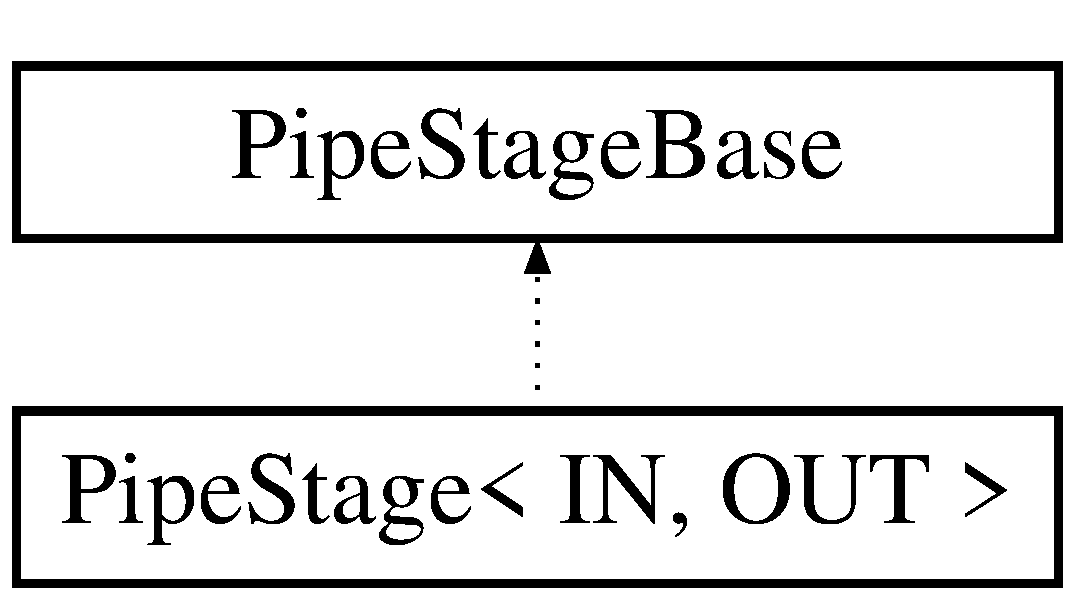
\includegraphics[height=2.000000cm]{classPipeStage}
\end{center}
\end{figure}
\subsection*{Public Member Functions}
\begin{DoxyCompactItemize}
\item 
void \hyperlink{classPipeStage_a8ec0fdc19a323ebac63755e6c47daabf}{execute} ()
\item 
virtual O\-U\-T \hyperlink{classPipeStage_ad3dc477759bf2c6cb866075a91a5089f}{run} (I\-N in)=0
\end{DoxyCompactItemize}
\subsection*{Public Attributes}
\begin{DoxyCompactItemize}
\item 
vector$<$ O\-U\-T $>$ $\ast$ \hyperlink{classPipeStage_ae35e3d09c1204f1fdcbb87fd97952885}{out\-Buffer}
\item 
vector$<$ I\-N $>$ \hyperlink{classPipeStage_a2dc9b1f5b98e6b0975cd06b899000078}{in\-Buffer}
\end{DoxyCompactItemize}


\subsection{Member Function Documentation}
\hypertarget{classPipeStage_a8ec0fdc19a323ebac63755e6c47daabf}{\index{Pipe\-Stage@{Pipe\-Stage}!execute@{execute}}
\index{execute@{execute}!PipeStage@{Pipe\-Stage}}
\subsubsection[{execute}]{\setlength{\rightskip}{0pt plus 5cm}template$<$typename I\-N, typename O\-U\-T$>$ void {\bf Pipe\-Stage}$<$ I\-N, O\-U\-T $>$\-::execute (
\begin{DoxyParamCaption}
{}
\end{DoxyParamCaption}
)\hspace{0.3cm}{\ttfamily [inline]}, {\ttfamily [virtual]}}}\label{classPipeStage_a8ec0fdc19a323ebac63755e6c47daabf}


Implements \hyperlink{classPipeStageBase}{Pipe\-Stage\-Base}.

\hypertarget{classPipeStage_ad3dc477759bf2c6cb866075a91a5089f}{\index{Pipe\-Stage@{Pipe\-Stage}!run@{run}}
\index{run@{run}!PipeStage@{Pipe\-Stage}}
\subsubsection[{run}]{\setlength{\rightskip}{0pt plus 5cm}template$<$typename I\-N, typename O\-U\-T$>$ virtual O\-U\-T {\bf Pipe\-Stage}$<$ I\-N, O\-U\-T $>$\-::run (
\begin{DoxyParamCaption}
\item[{I\-N}]{in}
\end{DoxyParamCaption}
)\hspace{0.3cm}{\ttfamily [pure virtual]}}}\label{classPipeStage_ad3dc477759bf2c6cb866075a91a5089f}


\subsection{Member Data Documentation}
\hypertarget{classPipeStage_a2dc9b1f5b98e6b0975cd06b899000078}{\index{Pipe\-Stage@{Pipe\-Stage}!in\-Buffer@{in\-Buffer}}
\index{in\-Buffer@{in\-Buffer}!PipeStage@{Pipe\-Stage}}
\subsubsection[{in\-Buffer}]{\setlength{\rightskip}{0pt plus 5cm}template$<$typename I\-N, typename O\-U\-T$>$ vector$<$I\-N$>$ {\bf Pipe\-Stage}$<$ I\-N, O\-U\-T $>$\-::in\-Buffer}}\label{classPipeStage_a2dc9b1f5b98e6b0975cd06b899000078}
\hypertarget{classPipeStage_ae35e3d09c1204f1fdcbb87fd97952885}{\index{Pipe\-Stage@{Pipe\-Stage}!out\-Buffer@{out\-Buffer}}
\index{out\-Buffer@{out\-Buffer}!PipeStage@{Pipe\-Stage}}
\subsubsection[{out\-Buffer}]{\setlength{\rightskip}{0pt plus 5cm}template$<$typename I\-N, typename O\-U\-T$>$ vector$<$O\-U\-T$>$$\ast$ {\bf Pipe\-Stage}$<$ I\-N, O\-U\-T $>$\-::out\-Buffer}}\label{classPipeStage_ae35e3d09c1204f1fdcbb87fd97952885}


The documentation for this class was generated from the following file\-:\begin{DoxyCompactItemize}
\item 
/afs/inf.\-ed.\-ac.\-uk/user/s18/s1837296/dev/stencil/\-Distribute/\hyperlink{Pipeline_8hpp}{Pipeline.\-hpp}\end{DoxyCompactItemize}

\hypertarget{classPipeStageBase}{\section{Pipe\-Stage\-Base Class Reference}
\label{classPipeStageBase}\index{Pipe\-Stage\-Base@{Pipe\-Stage\-Base}}
}


{\ttfamily \#include $<$Pipeline.\-hpp$>$}

Inheritance diagram for Pipe\-Stage\-Base\-:\begin{figure}[H]
\begin{center}
\leavevmode
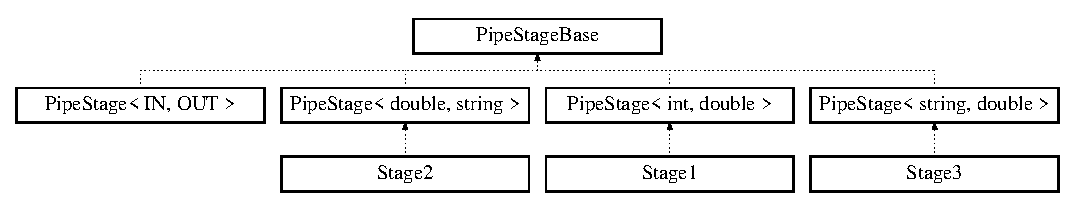
\includegraphics[height=2.346369cm]{classPipeStageBase}
\end{center}
\end{figure}


The documentation for this class was generated from the following file\-:\begin{DoxyCompactItemize}
\item 
/afs/inf.\-ed.\-ac.\-uk/user/s18/s1837296/dev/stencil/\-Distribute/\hyperlink{Pipeline_8hpp}{Pipeline.\-hpp}\end{DoxyCompactItemize}

\hypertarget{classReduceSkeleton_1_1ReduceImplementation}{\section{Reduce\-Skeleton\-:\-:Reduce\-Implementation$<$ C\-O $>$ Class Template Reference}
\label{classReduceSkeleton_1_1ReduceImplementation}\index{Reduce\-Skeleton\-::\-Reduce\-Implementation$<$ C\-O $>$@{Reduce\-Skeleton\-::\-Reduce\-Implementation$<$ C\-O $>$}}
}


{\ttfamily \#include $<$Reduce.\-hpp$>$}

\subsection*{Public Member Functions}
\begin{DoxyCompactItemize}
\item 
{\footnotesize template$<$typename I\-N , typename... A\-R\-Gs$>$ }\\void \hyperlink{classReduceSkeleton_1_1ReduceImplementation_a47458d1b1d6bf24c2e1ca6797c27bbc5}{operator()} (I\-N \&output, std\-::vector$<$ I\-N $>$ \&input, A\-R\-Gs...\-args)
\end{DoxyCompactItemize}
\subsection*{Friends}
\begin{DoxyCompactItemize}
\item 
{\footnotesize template$<$typename C\-O2 $>$ }\\\hyperlink{classReduceSkeleton_1_1ReduceImplementation}{Reduce\-Skeleton\-::\-Reduce\-Implementation}\\*
$<$ C\-O2 $>$ \hyperlink{classReduceSkeleton_1_1ReduceImplementation_afa20d0c393a3a0891c2b49f7cf96eaca}{\-\_\-\-\_\-\-Reduce\-With\-Access} (C\-O2 co, const size\-\_\-t \&threads)
\end{DoxyCompactItemize}


\subsection{Member Function Documentation}
\hypertarget{classReduceSkeleton_1_1ReduceImplementation_a47458d1b1d6bf24c2e1ca6797c27bbc5}{\index{Reduce\-Skeleton\-::\-Reduce\-Implementation@{Reduce\-Skeleton\-::\-Reduce\-Implementation}!operator()@{operator()}}
\index{operator()@{operator()}!ReduceSkeleton::ReduceImplementation@{Reduce\-Skeleton\-::\-Reduce\-Implementation}}
\subsubsection[{operator()}]{\setlength{\rightskip}{0pt plus 5cm}template$<$typename C\-O$>$ template$<$typename I\-N , typename... A\-R\-Gs$>$ void {\bf Reduce\-Skeleton\-::\-Reduce\-Implementation}$<$ C\-O $>$\-::operator() (
\begin{DoxyParamCaption}
\item[{I\-N \&}]{output, }
\item[{std\-::vector$<$ I\-N $>$ \&}]{input, }
\item[{A\-R\-Gs...}]{args}
\end{DoxyParamCaption}
)\hspace{0.3cm}{\ttfamily [inline]}}}\label{classReduceSkeleton_1_1ReduceImplementation_a47458d1b1d6bf24c2e1ca6797c27bbc5}


\subsection{Friends And Related Function Documentation}
\hypertarget{classReduceSkeleton_1_1ReduceImplementation_afa20d0c393a3a0891c2b49f7cf96eaca}{\index{Reduce\-Skeleton\-::\-Reduce\-Implementation@{Reduce\-Skeleton\-::\-Reduce\-Implementation}!\-\_\-\-\_\-\-Reduce\-With\-Access@{\-\_\-\-\_\-\-Reduce\-With\-Access}}
\index{\-\_\-\-\_\-\-Reduce\-With\-Access@{\-\_\-\-\_\-\-Reduce\-With\-Access}!ReduceSkeleton::ReduceImplementation@{Reduce\-Skeleton\-::\-Reduce\-Implementation}}
\subsubsection[{\-\_\-\-\_\-\-Reduce\-With\-Access}]{\setlength{\rightskip}{0pt plus 5cm}template$<$typename C\-O$>$ template$<$typename C\-O2 $>$ {\bf Reduce\-Skeleton\-::\-Reduce\-Implementation}$<$C\-O2$>$ \-\_\-\-\_\-\-Reduce\-With\-Access (
\begin{DoxyParamCaption}
\item[{C\-O2}]{co, }
\item[{const size\-\_\-t \&}]{threads}
\end{DoxyParamCaption}
)\hspace{0.3cm}{\ttfamily [friend]}}}\label{classReduceSkeleton_1_1ReduceImplementation_afa20d0c393a3a0891c2b49f7cf96eaca}


The documentation for this class was generated from the following file\-:\begin{DoxyCompactItemize}
\item 
/afs/inf.\-ed.\-ac.\-uk/user/s18/s1837296/dev/stencil/\-Distribute/\hyperlink{Reduce_8hpp}{Reduce.\-hpp}\end{DoxyCompactItemize}

\hypertarget{classReduceSkeleton}{\section{Reduce\-Skeleton Class Reference}
\label{classReduceSkeleton}\index{Reduce\-Skeleton@{Reduce\-Skeleton}}
}


{\ttfamily \#include $<$Reduce.\-hpp$>$}

\subsection*{Classes}
\begin{DoxyCompactItemize}
\item 
class \hyperlink{classReduceSkeleton_1_1ReduceImplementation}{Reduce\-Implementation}
\end{DoxyCompactItemize}
\subsection*{Friends}
\begin{DoxyCompactItemize}
\item 
{\footnotesize template$<$typename C\-O2 $>$ }\\\hyperlink{classReduceSkeleton_1_1ReduceImplementation}{Reduce\-Skeleton\-::\-Reduce\-Implementation}\\*
$<$ C\-O2 $>$ \hyperlink{classReduceSkeleton_afa20d0c393a3a0891c2b49f7cf96eaca}{\-\_\-\-\_\-\-Reduce\-With\-Access} (C\-O2 co, const size\-\_\-t \&threads)
\end{DoxyCompactItemize}


\subsection{Friends And Related Function Documentation}
\hypertarget{classReduceSkeleton_afa20d0c393a3a0891c2b49f7cf96eaca}{\index{Reduce\-Skeleton@{Reduce\-Skeleton}!\-\_\-\-\_\-\-Reduce\-With\-Access@{\-\_\-\-\_\-\-Reduce\-With\-Access}}
\index{\-\_\-\-\_\-\-Reduce\-With\-Access@{\-\_\-\-\_\-\-Reduce\-With\-Access}!ReduceSkeleton@{Reduce\-Skeleton}}
\subsubsection[{\-\_\-\-\_\-\-Reduce\-With\-Access}]{\setlength{\rightskip}{0pt plus 5cm}template$<$typename C\-O2 $>$ {\bf Reduce\-Skeleton\-::\-Reduce\-Implementation}$<$C\-O2$>$ \-\_\-\-\_\-\-Reduce\-With\-Access (
\begin{DoxyParamCaption}
\item[{C\-O2}]{co, }
\item[{const size\-\_\-t \&}]{threads}
\end{DoxyParamCaption}
)\hspace{0.3cm}{\ttfamily [friend]}}}\label{classReduceSkeleton_afa20d0c393a3a0891c2b49f7cf96eaca}


The documentation for this class was generated from the following file\-:\begin{DoxyCompactItemize}
\item 
/afs/inf.\-ed.\-ac.\-uk/user/s18/s1837296/dev/stencil/\-Distribute/\hyperlink{Reduce_8hpp}{Reduce.\-hpp}\end{DoxyCompactItemize}

\hypertarget{classScanSkeleton_1_1ScanImplementation}{\section{Scan\-Skeleton\-:\-:Scan\-Implementation$<$ S\-U $>$ Class Template Reference}
\label{classScanSkeleton_1_1ScanImplementation}\index{Scan\-Skeleton\-::\-Scan\-Implementation$<$ S\-U $>$@{Scan\-Skeleton\-::\-Scan\-Implementation$<$ S\-U $>$}}
}


{\ttfamily \#include $<$Scan.\-hpp$>$}

\subsection*{Public Member Functions}
\begin{DoxyCompactItemize}
\item 
{\footnotesize template$<$typename I\-N , typename... A\-R\-Gs$>$ }\\void \hyperlink{classScanSkeleton_1_1ScanImplementation_a83b315d3ff4dcb1a82fcbce95194b0ba}{operator()} (std\-::vector$<$ I\-N $>$ \&output, std\-::vector$<$ I\-N $>$ input, A\-R\-Gs...\-args)
\end{DoxyCompactItemize}
\subsection*{Friends}
\begin{DoxyCompactItemize}
\item 
{\footnotesize template$<$typename S\-U2 $>$ }\\\hyperlink{classScanSkeleton_1_1ScanImplementation}{Scan\-Skeleton\-::\-Scan\-Implementation}\\*
$<$ S\-U2 $>$ \hyperlink{classScanSkeleton_1_1ScanImplementation_abe3a3f160ae7b38ff94db7eab167ecf1}{\-\_\-\-\_\-\-Scan\-With\-Access} (S\-U2 su, const size\-\_\-t \&threads)
\end{DoxyCompactItemize}


\subsection{Detailed Description}
\subsubsection*{template$<$typename S\-U$>$class Scan\-Skeleton\-::\-Scan\-Implementation$<$ S\-U $>$}

\hyperlink{classScanSkeleton_1_1ScanImplementation}{Scan\-Implementation} 

\subsection{Member Function Documentation}
\hypertarget{classScanSkeleton_1_1ScanImplementation_a83b315d3ff4dcb1a82fcbce95194b0ba}{\index{Scan\-Skeleton\-::\-Scan\-Implementation@{Scan\-Skeleton\-::\-Scan\-Implementation}!operator()@{operator()}}
\index{operator()@{operator()}!ScanSkeleton::ScanImplementation@{Scan\-Skeleton\-::\-Scan\-Implementation}}
\subsubsection[{operator()}]{\setlength{\rightskip}{0pt plus 5cm}template$<$typename S\-U$>$ template$<$typename I\-N , typename... A\-R\-Gs$>$ void {\bf Scan\-Skeleton\-::\-Scan\-Implementation}$<$ S\-U $>$\-::operator() (
\begin{DoxyParamCaption}
\item[{std\-::vector$<$ I\-N $>$ \&}]{output, }
\item[{std\-::vector$<$ I\-N $>$}]{input, }
\item[{A\-R\-Gs...}]{args}
\end{DoxyParamCaption}
)\hspace{0.3cm}{\ttfamily [inline]}}}\label{classScanSkeleton_1_1ScanImplementation_a83b315d3ff4dcb1a82fcbce95194b0ba}


\subsection{Friends And Related Function Documentation}
\hypertarget{classScanSkeleton_1_1ScanImplementation_abe3a3f160ae7b38ff94db7eab167ecf1}{\index{Scan\-Skeleton\-::\-Scan\-Implementation@{Scan\-Skeleton\-::\-Scan\-Implementation}!\-\_\-\-\_\-\-Scan\-With\-Access@{\-\_\-\-\_\-\-Scan\-With\-Access}}
\index{\-\_\-\-\_\-\-Scan\-With\-Access@{\-\_\-\-\_\-\-Scan\-With\-Access}!ScanSkeleton::ScanImplementation@{Scan\-Skeleton\-::\-Scan\-Implementation}}
\subsubsection[{\-\_\-\-\_\-\-Scan\-With\-Access}]{\setlength{\rightskip}{0pt plus 5cm}template$<$typename S\-U$>$ template$<$typename S\-U2 $>$ {\bf Scan\-Skeleton\-::\-Scan\-Implementation}$<$S\-U2$>$ \-\_\-\-\_\-\-Scan\-With\-Access (
\begin{DoxyParamCaption}
\item[{S\-U2}]{su, }
\item[{const size\-\_\-t \&}]{threads}
\end{DoxyParamCaption}
)\hspace{0.3cm}{\ttfamily [friend]}}}\label{classScanSkeleton_1_1ScanImplementation_abe3a3f160ae7b38ff94db7eab167ecf1}


The documentation for this class was generated from the following file\-:\begin{DoxyCompactItemize}
\item 
/afs/inf.\-ed.\-ac.\-uk/user/s18/s1837296/dev/stencil/\-Distribute/\hyperlink{Scan_8hpp}{Scan.\-hpp}\end{DoxyCompactItemize}

\hypertarget{classScanSkeleton}{\section{Scan\-Skeleton Class Reference}
\label{classScanSkeleton}\index{Scan\-Skeleton@{Scan\-Skeleton}}
}


{\ttfamily \#include $<$Scan.\-hpp$>$}

\subsection*{Classes}
\begin{DoxyCompactItemize}
\item 
class \hyperlink{classScanSkeleton_1_1ScanImplementation}{Scan\-Implementation}
\end{DoxyCompactItemize}
\subsection*{Friends}
\begin{DoxyCompactItemize}
\item 
{\footnotesize template$<$typename S\-U2 $>$ }\\\hyperlink{classScanSkeleton_1_1ScanImplementation}{Scan\-Skeleton\-::\-Scan\-Implementation}\\*
$<$ S\-U2 $>$ \hyperlink{classScanSkeleton_abe3a3f160ae7b38ff94db7eab167ecf1}{\-\_\-\-\_\-\-Scan\-With\-Access} (S\-U2 su, const size\-\_\-t \&threads)
\end{DoxyCompactItemize}


\subsection{Friends And Related Function Documentation}
\hypertarget{classScanSkeleton_abe3a3f160ae7b38ff94db7eab167ecf1}{\index{Scan\-Skeleton@{Scan\-Skeleton}!\-\_\-\-\_\-\-Scan\-With\-Access@{\-\_\-\-\_\-\-Scan\-With\-Access}}
\index{\-\_\-\-\_\-\-Scan\-With\-Access@{\-\_\-\-\_\-\-Scan\-With\-Access}!ScanSkeleton@{Scan\-Skeleton}}
\subsubsection[{\-\_\-\-\_\-\-Scan\-With\-Access}]{\setlength{\rightskip}{0pt plus 5cm}template$<$typename S\-U2 $>$ {\bf Scan\-Skeleton\-::\-Scan\-Implementation}$<$S\-U2$>$ \-\_\-\-\_\-\-Scan\-With\-Access (
\begin{DoxyParamCaption}
\item[{S\-U2}]{su, }
\item[{const size\-\_\-t \&}]{threads}
\end{DoxyParamCaption}
)\hspace{0.3cm}{\ttfamily [friend]}}}\label{classScanSkeleton_abe3a3f160ae7b38ff94db7eab167ecf1}


The documentation for this class was generated from the following file\-:\begin{DoxyCompactItemize}
\item 
/afs/inf.\-ed.\-ac.\-uk/user/s18/s1837296/dev/stencil/\-Distribute/\hyperlink{Scan_8hpp}{Scan.\-hpp}\end{DoxyCompactItemize}

\hypertarget{classStage1}{\section{Stage1 Class Reference}
\label{classStage1}\index{Stage1@{Stage1}}
}


{\ttfamily \#include $<$Pipeline.\-hpp$>$}

Inheritance diagram for Stage1\-:\begin{figure}[H]
\begin{center}
\leavevmode
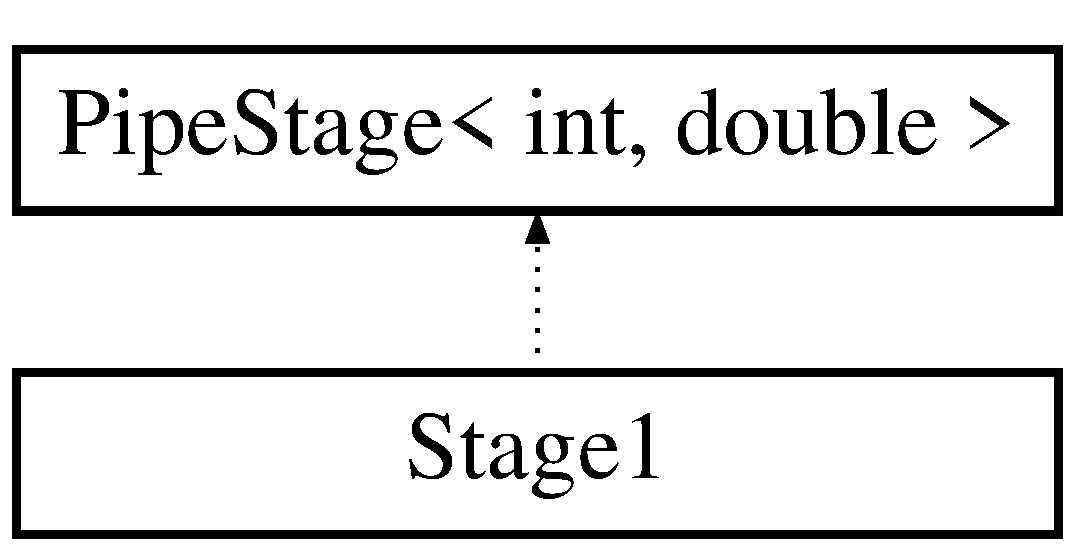
\includegraphics[height=2.000000cm]{classStage1}
\end{center}
\end{figure}


The documentation for this class was generated from the following file\-:\begin{DoxyCompactItemize}
\item 
/afs/inf.\-ed.\-ac.\-uk/user/s18/s1837296/dev/stencil/\-Distribute/\hyperlink{Pipeline_8hpp}{Pipeline.\-hpp}\end{DoxyCompactItemize}

\hypertarget{classStage2}{\section{Stage2 Class Reference}
\label{classStage2}\index{Stage2@{Stage2}}
}


{\ttfamily \#include $<$Pipeline.\-hpp$>$}

Inheritance diagram for Stage2\-:\begin{figure}[H]
\begin{center}
\leavevmode
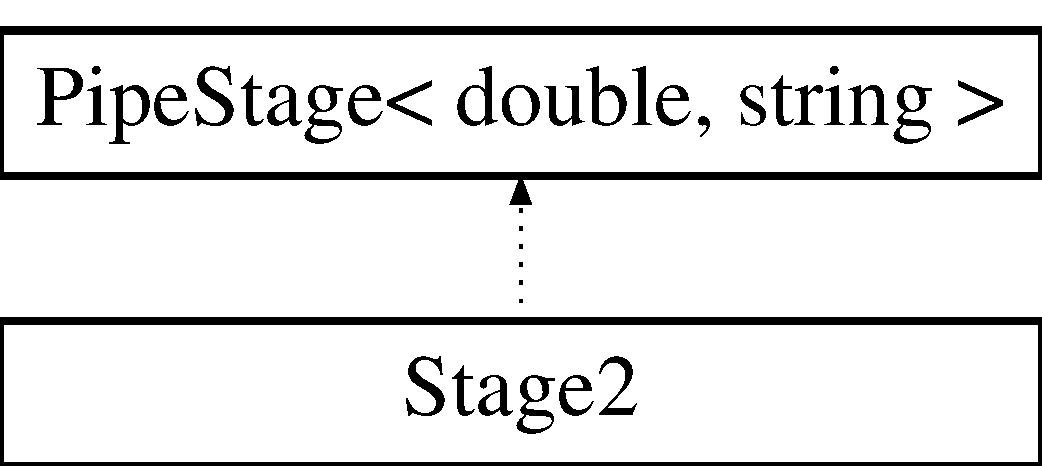
\includegraphics[height=2.000000cm]{classStage2}
\end{center}
\end{figure}


The documentation for this class was generated from the following file\-:\begin{DoxyCompactItemize}
\item 
/afs/inf.\-ed.\-ac.\-uk/user/s18/s1837296/dev/stencil/\-Distribute/\hyperlink{Pipeline_8hpp}{Pipeline.\-hpp}\end{DoxyCompactItemize}

\hypertarget{classStage3}{\section{Stage3 Class Reference}
\label{classStage3}\index{Stage3@{Stage3}}
}


{\ttfamily \#include $<$Pipeline.\-hpp$>$}

Inheritance diagram for Stage3\-:\begin{figure}[H]
\begin{center}
\leavevmode
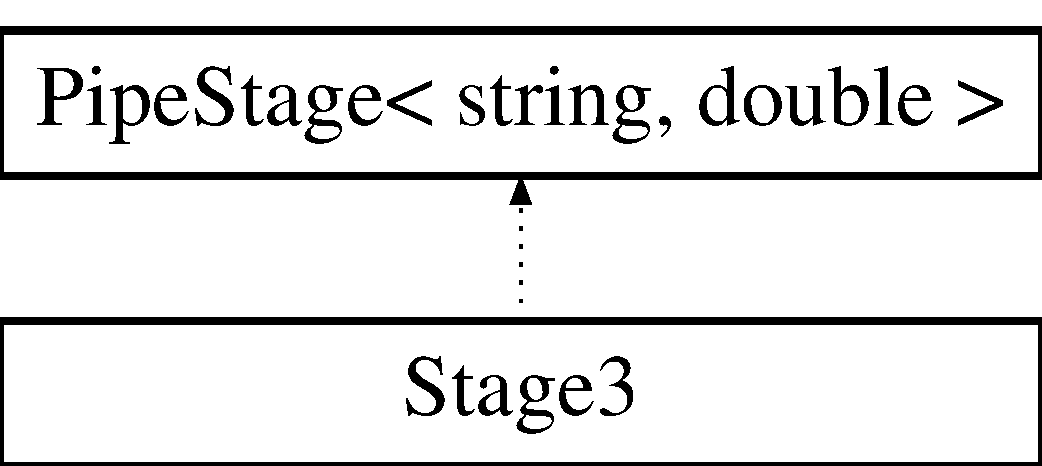
\includegraphics[height=2.000000cm]{classStage3}
\end{center}
\end{figure}


The documentation for this class was generated from the following file\-:\begin{DoxyCompactItemize}
\item 
/afs/inf.\-ed.\-ac.\-uk/user/s18/s1837296/dev/stencil/\-Distribute/\hyperlink{Pipeline_8hpp}{Pipeline.\-hpp}\end{DoxyCompactItemize}

\hypertarget{classStencilSkeleton_1_1StencilImplementation}{\section{Stencil\-Skeleton\-:\-:Stencil\-Implementation$<$ E\-L $>$ Class Template Reference}
\label{classStencilSkeleton_1_1StencilImplementation}\index{Stencil\-Skeleton\-::\-Stencil\-Implementation$<$ E\-L $>$@{Stencil\-Skeleton\-::\-Stencil\-Implementation$<$ E\-L $>$}}
}


{\ttfamily \#include $<$Stencil.\-hpp$>$}



The documentation for this class was generated from the following file\-:\begin{DoxyCompactItemize}
\item 
/afs/inf.\-ed.\-ac.\-uk/user/s18/s1837296/dev/stencil/\-Distribute/\hyperlink{Stencil_8hpp}{Stencil.\-hpp}\end{DoxyCompactItemize}

\hypertarget{classStencilSkeleton}{\section{Stencil\-Skeleton Class Reference}
\label{classStencilSkeleton}\index{Stencil\-Skeleton@{Stencil\-Skeleton}}
}


{\ttfamily \#include $<$Stencil.\-hpp$>$}

\subsection*{Classes}
\begin{DoxyCompactItemize}
\item 
class \hyperlink{classStencilSkeleton_1_1StencilImplementation}{Stencil\-Implementation}
\end{DoxyCompactItemize}


The documentation for this class was generated from the following file\-:\begin{DoxyCompactItemize}
\item 
/afs/inf.\-ed.\-ac.\-uk/user/s18/s1837296/dev/stencil/\-Distribute/\hyperlink{Stencil_8hpp}{Stencil.\-hpp}\end{DoxyCompactItemize}

\hypertarget{classKMeans_1_1ThreadArgClosestCentroid}{\section{K\-Means\-:\-:Thread\-Arg\-Closest\-Centroid Class Reference}
\label{classKMeans_1_1ThreadArgClosestCentroid}\index{K\-Means\-::\-Thread\-Arg\-Closest\-Centroid@{K\-Means\-::\-Thread\-Arg\-Closest\-Centroid}}
}
\subsection*{Public Attributes}
\begin{DoxyCompactItemize}
\item 
std\-::vector$<$ \hyperlink{structKMeans_1_1KMPoint}{K\-M\-Point} $\ast$ $>$ $\ast$ \hyperlink{classKMeans_1_1ThreadArgClosestCentroid_ab5aa69fc9a81c813c6a4836679e698f8}{input}
\item 
std\-::vector$<$ \hyperlink{structKMeans_1_1KMPoint}{K\-M\-Point} $>$ $\ast$ \hyperlink{classKMeans_1_1ThreadArgClosestCentroid_a3430e65d878b25d8b96a7e663be62e82}{centroids}
\item 
size\-\_\-t $\ast$ \hyperlink{classKMeans_1_1ThreadArgClosestCentroid_a84cc9890531db34f34e5c008c55a6d0a}{chunk\-Indices}
\end{DoxyCompactItemize}


\subsection{Member Data Documentation}
\hypertarget{classKMeans_1_1ThreadArgClosestCentroid_a3430e65d878b25d8b96a7e663be62e82}{\index{K\-Means\-::\-Thread\-Arg\-Closest\-Centroid@{K\-Means\-::\-Thread\-Arg\-Closest\-Centroid}!centroids@{centroids}}
\index{centroids@{centroids}!KMeans::ThreadArgClosestCentroid@{K\-Means\-::\-Thread\-Arg\-Closest\-Centroid}}
\subsubsection[{centroids}]{\setlength{\rightskip}{0pt plus 5cm}std\-::vector$<${\bf K\-M\-Point}$>$$\ast$ K\-Means\-::\-Thread\-Arg\-Closest\-Centroid\-::centroids}}\label{classKMeans_1_1ThreadArgClosestCentroid_a3430e65d878b25d8b96a7e663be62e82}
\hypertarget{classKMeans_1_1ThreadArgClosestCentroid_a84cc9890531db34f34e5c008c55a6d0a}{\index{K\-Means\-::\-Thread\-Arg\-Closest\-Centroid@{K\-Means\-::\-Thread\-Arg\-Closest\-Centroid}!chunk\-Indices@{chunk\-Indices}}
\index{chunk\-Indices@{chunk\-Indices}!KMeans::ThreadArgClosestCentroid@{K\-Means\-::\-Thread\-Arg\-Closest\-Centroid}}
\subsubsection[{chunk\-Indices}]{\setlength{\rightskip}{0pt plus 5cm}size\-\_\-t$\ast$ K\-Means\-::\-Thread\-Arg\-Closest\-Centroid\-::chunk\-Indices}}\label{classKMeans_1_1ThreadArgClosestCentroid_a84cc9890531db34f34e5c008c55a6d0a}
\hypertarget{classKMeans_1_1ThreadArgClosestCentroid_ab5aa69fc9a81c813c6a4836679e698f8}{\index{K\-Means\-::\-Thread\-Arg\-Closest\-Centroid@{K\-Means\-::\-Thread\-Arg\-Closest\-Centroid}!input@{input}}
\index{input@{input}!KMeans::ThreadArgClosestCentroid@{K\-Means\-::\-Thread\-Arg\-Closest\-Centroid}}
\subsubsection[{input}]{\setlength{\rightskip}{0pt plus 5cm}std\-::vector$<${\bf K\-M\-Point}$\ast$$>$$\ast$ K\-Means\-::\-Thread\-Arg\-Closest\-Centroid\-::input}}\label{classKMeans_1_1ThreadArgClosestCentroid_ab5aa69fc9a81c813c6a4836679e698f8}


The documentation for this class was generated from the following file\-:\begin{DoxyCompactItemize}
\item 
/afs/inf.\-ed.\-ac.\-uk/user/s18/s1837296/dev/stencil/\-Distribute/\hyperlink{problemKmeans_8cpp}{problem\-Kmeans.\-cpp}\end{DoxyCompactItemize}

\hypertarget{classSummedArea_1_1ThreadArgGetArea}{\section{Summed\-Area\-:\-:Thread\-Arg\-Get\-Area Class Reference}
\label{classSummedArea_1_1ThreadArgGetArea}\index{Summed\-Area\-::\-Thread\-Arg\-Get\-Area@{Summed\-Area\-::\-Thread\-Arg\-Get\-Area}}
}
\subsection*{Public Attributes}
\begin{DoxyCompactItemize}
\item 
size\-\_\-t \hyperlink{classSummedArea_1_1ThreadArgGetArea_af67fa94677c2947d70ba11a42b923d36}{sample\-Index\-Start}
\item 
size\-\_\-t \hyperlink{classSummedArea_1_1ThreadArgGetArea_ab0d261bfd483b3b5c790bcec68535e36}{sample\-Index\-End}
\item 
double \hyperlink{classSummedArea_1_1ThreadArgGetArea_a5c177ecad27b4a1bf6109bbc98f33bc3}{dx}
\item 
int \hyperlink{classSummedArea_1_1ThreadArgGetArea_a9f42d9e54909749f1e278e1954330d89}{n}
\item 
std\-::vector$<$ double $>$ $\ast$ \hyperlink{classSummedArea_1_1ThreadArgGetArea_ad37fc357e9602189579bfe9e352d4041}{samples}
\item 
std\-::vector$<$ double $>$ $\ast$ \hyperlink{classSummedArea_1_1ThreadArgGetArea_ae7740ca6e8e204044dedbdc9ce25fe97}{sample\-Area}
\end{DoxyCompactItemize}


\subsection{Member Data Documentation}
\hypertarget{classSummedArea_1_1ThreadArgGetArea_a5c177ecad27b4a1bf6109bbc98f33bc3}{\index{Summed\-Area\-::\-Thread\-Arg\-Get\-Area@{Summed\-Area\-::\-Thread\-Arg\-Get\-Area}!dx@{dx}}
\index{dx@{dx}!SummedArea::ThreadArgGetArea@{Summed\-Area\-::\-Thread\-Arg\-Get\-Area}}
\subsubsection[{dx}]{\setlength{\rightskip}{0pt plus 5cm}double Summed\-Area\-::\-Thread\-Arg\-Get\-Area\-::dx}}\label{classSummedArea_1_1ThreadArgGetArea_a5c177ecad27b4a1bf6109bbc98f33bc3}
\hypertarget{classSummedArea_1_1ThreadArgGetArea_a9f42d9e54909749f1e278e1954330d89}{\index{Summed\-Area\-::\-Thread\-Arg\-Get\-Area@{Summed\-Area\-::\-Thread\-Arg\-Get\-Area}!n@{n}}
\index{n@{n}!SummedArea::ThreadArgGetArea@{Summed\-Area\-::\-Thread\-Arg\-Get\-Area}}
\subsubsection[{n}]{\setlength{\rightskip}{0pt plus 5cm}int Summed\-Area\-::\-Thread\-Arg\-Get\-Area\-::n}}\label{classSummedArea_1_1ThreadArgGetArea_a9f42d9e54909749f1e278e1954330d89}
\hypertarget{classSummedArea_1_1ThreadArgGetArea_ae7740ca6e8e204044dedbdc9ce25fe97}{\index{Summed\-Area\-::\-Thread\-Arg\-Get\-Area@{Summed\-Area\-::\-Thread\-Arg\-Get\-Area}!sample\-Area@{sample\-Area}}
\index{sample\-Area@{sample\-Area}!SummedArea::ThreadArgGetArea@{Summed\-Area\-::\-Thread\-Arg\-Get\-Area}}
\subsubsection[{sample\-Area}]{\setlength{\rightskip}{0pt plus 5cm}std\-::vector$<$double$>$$\ast$ Summed\-Area\-::\-Thread\-Arg\-Get\-Area\-::sample\-Area}}\label{classSummedArea_1_1ThreadArgGetArea_ae7740ca6e8e204044dedbdc9ce25fe97}
\hypertarget{classSummedArea_1_1ThreadArgGetArea_ab0d261bfd483b3b5c790bcec68535e36}{\index{Summed\-Area\-::\-Thread\-Arg\-Get\-Area@{Summed\-Area\-::\-Thread\-Arg\-Get\-Area}!sample\-Index\-End@{sample\-Index\-End}}
\index{sample\-Index\-End@{sample\-Index\-End}!SummedArea::ThreadArgGetArea@{Summed\-Area\-::\-Thread\-Arg\-Get\-Area}}
\subsubsection[{sample\-Index\-End}]{\setlength{\rightskip}{0pt plus 5cm}size\-\_\-t Summed\-Area\-::\-Thread\-Arg\-Get\-Area\-::sample\-Index\-End}}\label{classSummedArea_1_1ThreadArgGetArea_ab0d261bfd483b3b5c790bcec68535e36}
\hypertarget{classSummedArea_1_1ThreadArgGetArea_af67fa94677c2947d70ba11a42b923d36}{\index{Summed\-Area\-::\-Thread\-Arg\-Get\-Area@{Summed\-Area\-::\-Thread\-Arg\-Get\-Area}!sample\-Index\-Start@{sample\-Index\-Start}}
\index{sample\-Index\-Start@{sample\-Index\-Start}!SummedArea::ThreadArgGetArea@{Summed\-Area\-::\-Thread\-Arg\-Get\-Area}}
\subsubsection[{sample\-Index\-Start}]{\setlength{\rightskip}{0pt plus 5cm}size\-\_\-t Summed\-Area\-::\-Thread\-Arg\-Get\-Area\-::sample\-Index\-Start}}\label{classSummedArea_1_1ThreadArgGetArea_af67fa94677c2947d70ba11a42b923d36}
\hypertarget{classSummedArea_1_1ThreadArgGetArea_ad37fc357e9602189579bfe9e352d4041}{\index{Summed\-Area\-::\-Thread\-Arg\-Get\-Area@{Summed\-Area\-::\-Thread\-Arg\-Get\-Area}!samples@{samples}}
\index{samples@{samples}!SummedArea::ThreadArgGetArea@{Summed\-Area\-::\-Thread\-Arg\-Get\-Area}}
\subsubsection[{samples}]{\setlength{\rightskip}{0pt plus 5cm}std\-::vector$<$double$>$$\ast$ Summed\-Area\-::\-Thread\-Arg\-Get\-Area\-::samples}}\label{classSummedArea_1_1ThreadArgGetArea_ad37fc357e9602189579bfe9e352d4041}


The documentation for this class was generated from the following file\-:\begin{DoxyCompactItemize}
\item 
/afs/inf.\-ed.\-ac.\-uk/user/s18/s1837296/dev/stencil/\-Distribute/\hyperlink{problemSummedArea_8cpp}{problem\-Summed\-Area.\-cpp}\end{DoxyCompactItemize}

\hypertarget{classSummedArea_1_1ThreadArgGetSummedArea}{\section{Summed\-Area\-:\-:Thread\-Arg\-Get\-Summed\-Area Class Reference}
\label{classSummedArea_1_1ThreadArgGetSummedArea}\index{Summed\-Area\-::\-Thread\-Arg\-Get\-Summed\-Area@{Summed\-Area\-::\-Thread\-Arg\-Get\-Summed\-Area}}
}
\subsection*{Public Attributes}
\begin{DoxyCompactItemize}
\item 
size\-\_\-t \hyperlink{classSummedArea_1_1ThreadArgGetSummedArea_a6b09db7eb9a63d224a6a30ff3ddda5a9}{chunk\-Start}
\item 
size\-\_\-t \hyperlink{classSummedArea_1_1ThreadArgGetSummedArea_a2d54148cc8b8339f10d09788c023c20a}{chunk\-End}
\item 
std\-::vector$<$ double $>$ $\ast$ \hyperlink{classSummedArea_1_1ThreadArgGetSummedArea_a259ec50cc8a157c409e607ef0cc985a7}{sample\-Area}
\item 
std\-::vector$<$ double $>$ $\ast$ \hyperlink{classSummedArea_1_1ThreadArgGetSummedArea_a1d372c5cf76441376dc475005c904ecb}{summed\-Area}
\end{DoxyCompactItemize}


\subsection{Member Data Documentation}
\hypertarget{classSummedArea_1_1ThreadArgGetSummedArea_a2d54148cc8b8339f10d09788c023c20a}{\index{Summed\-Area\-::\-Thread\-Arg\-Get\-Summed\-Area@{Summed\-Area\-::\-Thread\-Arg\-Get\-Summed\-Area}!chunk\-End@{chunk\-End}}
\index{chunk\-End@{chunk\-End}!SummedArea::ThreadArgGetSummedArea@{Summed\-Area\-::\-Thread\-Arg\-Get\-Summed\-Area}}
\subsubsection[{chunk\-End}]{\setlength{\rightskip}{0pt plus 5cm}size\-\_\-t Summed\-Area\-::\-Thread\-Arg\-Get\-Summed\-Area\-::chunk\-End}}\label{classSummedArea_1_1ThreadArgGetSummedArea_a2d54148cc8b8339f10d09788c023c20a}
\hypertarget{classSummedArea_1_1ThreadArgGetSummedArea_a6b09db7eb9a63d224a6a30ff3ddda5a9}{\index{Summed\-Area\-::\-Thread\-Arg\-Get\-Summed\-Area@{Summed\-Area\-::\-Thread\-Arg\-Get\-Summed\-Area}!chunk\-Start@{chunk\-Start}}
\index{chunk\-Start@{chunk\-Start}!SummedArea::ThreadArgGetSummedArea@{Summed\-Area\-::\-Thread\-Arg\-Get\-Summed\-Area}}
\subsubsection[{chunk\-Start}]{\setlength{\rightskip}{0pt plus 5cm}size\-\_\-t Summed\-Area\-::\-Thread\-Arg\-Get\-Summed\-Area\-::chunk\-Start}}\label{classSummedArea_1_1ThreadArgGetSummedArea_a6b09db7eb9a63d224a6a30ff3ddda5a9}
\hypertarget{classSummedArea_1_1ThreadArgGetSummedArea_a259ec50cc8a157c409e607ef0cc985a7}{\index{Summed\-Area\-::\-Thread\-Arg\-Get\-Summed\-Area@{Summed\-Area\-::\-Thread\-Arg\-Get\-Summed\-Area}!sample\-Area@{sample\-Area}}
\index{sample\-Area@{sample\-Area}!SummedArea::ThreadArgGetSummedArea@{Summed\-Area\-::\-Thread\-Arg\-Get\-Summed\-Area}}
\subsubsection[{sample\-Area}]{\setlength{\rightskip}{0pt plus 5cm}std\-::vector$<$double$>$$\ast$ Summed\-Area\-::\-Thread\-Arg\-Get\-Summed\-Area\-::sample\-Area}}\label{classSummedArea_1_1ThreadArgGetSummedArea_a259ec50cc8a157c409e607ef0cc985a7}
\hypertarget{classSummedArea_1_1ThreadArgGetSummedArea_a1d372c5cf76441376dc475005c904ecb}{\index{Summed\-Area\-::\-Thread\-Arg\-Get\-Summed\-Area@{Summed\-Area\-::\-Thread\-Arg\-Get\-Summed\-Area}!summed\-Area@{summed\-Area}}
\index{summed\-Area@{summed\-Area}!SummedArea::ThreadArgGetSummedArea@{Summed\-Area\-::\-Thread\-Arg\-Get\-Summed\-Area}}
\subsubsection[{summed\-Area}]{\setlength{\rightskip}{0pt plus 5cm}std\-::vector$<$double$>$$\ast$ Summed\-Area\-::\-Thread\-Arg\-Get\-Summed\-Area\-::summed\-Area}}\label{classSummedArea_1_1ThreadArgGetSummedArea_a1d372c5cf76441376dc475005c904ecb}


The documentation for this class was generated from the following file\-:\begin{DoxyCompactItemize}
\item 
/afs/inf.\-ed.\-ac.\-uk/user/s18/s1837296/dev/stencil/\-Distribute/\hyperlink{problemSummedArea_8cpp}{problem\-Summed\-Area.\-cpp}\end{DoxyCompactItemize}

\hypertarget{classKMeans_1_1ThreadArgNewCentroid}{\section{K\-Means\-:\-:Thread\-Arg\-New\-Centroid Class Reference}
\label{classKMeans_1_1ThreadArgNewCentroid}\index{K\-Means\-::\-Thread\-Arg\-New\-Centroid@{K\-Means\-::\-Thread\-Arg\-New\-Centroid}}
}
\subsection*{Public Attributes}
\begin{DoxyCompactItemize}
\item 
size\-\_\-t $\ast$ \hyperlink{classKMeans_1_1ThreadArgNewCentroid_ac026174de7fc8a7ca4a0c5b20b9e971d}{chunk\-Indices}
\item 
std\-::vector$<$ \hyperlink{structKMeans_1_1KMPoint}{K\-M\-Point} $\ast$ $>$ $\ast$ \hyperlink{classKMeans_1_1ThreadArgNewCentroid_afefa482db4fb35d1f498fec601aaa5e3}{input}
\item 
\hyperlink{structKMeans_1_1KMPoint}{K\-M\-Point} \hyperlink{classKMeans_1_1ThreadArgNewCentroid_a3c916ccdf617487a5b91578572241a36}{centroid}
\end{DoxyCompactItemize}


\subsection{Member Data Documentation}
\hypertarget{classKMeans_1_1ThreadArgNewCentroid_a3c916ccdf617487a5b91578572241a36}{\index{K\-Means\-::\-Thread\-Arg\-New\-Centroid@{K\-Means\-::\-Thread\-Arg\-New\-Centroid}!centroid@{centroid}}
\index{centroid@{centroid}!KMeans::ThreadArgNewCentroid@{K\-Means\-::\-Thread\-Arg\-New\-Centroid}}
\subsubsection[{centroid}]{\setlength{\rightskip}{0pt plus 5cm}{\bf K\-M\-Point} K\-Means\-::\-Thread\-Arg\-New\-Centroid\-::centroid}}\label{classKMeans_1_1ThreadArgNewCentroid_a3c916ccdf617487a5b91578572241a36}
\hypertarget{classKMeans_1_1ThreadArgNewCentroid_ac026174de7fc8a7ca4a0c5b20b9e971d}{\index{K\-Means\-::\-Thread\-Arg\-New\-Centroid@{K\-Means\-::\-Thread\-Arg\-New\-Centroid}!chunk\-Indices@{chunk\-Indices}}
\index{chunk\-Indices@{chunk\-Indices}!KMeans::ThreadArgNewCentroid@{K\-Means\-::\-Thread\-Arg\-New\-Centroid}}
\subsubsection[{chunk\-Indices}]{\setlength{\rightskip}{0pt plus 5cm}size\-\_\-t$\ast$ K\-Means\-::\-Thread\-Arg\-New\-Centroid\-::chunk\-Indices}}\label{classKMeans_1_1ThreadArgNewCentroid_ac026174de7fc8a7ca4a0c5b20b9e971d}
\hypertarget{classKMeans_1_1ThreadArgNewCentroid_afefa482db4fb35d1f498fec601aaa5e3}{\index{K\-Means\-::\-Thread\-Arg\-New\-Centroid@{K\-Means\-::\-Thread\-Arg\-New\-Centroid}!input@{input}}
\index{input@{input}!KMeans::ThreadArgNewCentroid@{K\-Means\-::\-Thread\-Arg\-New\-Centroid}}
\subsubsection[{input}]{\setlength{\rightskip}{0pt plus 5cm}std\-::vector$<${\bf K\-M\-Point} $\ast$$>$$\ast$ K\-Means\-::\-Thread\-Arg\-New\-Centroid\-::input}}\label{classKMeans_1_1ThreadArgNewCentroid_afefa482db4fb35d1f498fec601aaa5e3}


The documentation for this class was generated from the following file\-:\begin{DoxyCompactItemize}
\item 
/afs/inf.\-ed.\-ac.\-uk/user/s18/s1837296/dev/stencil/\-Distribute/\hyperlink{problemKmeans_8cpp}{problem\-Kmeans.\-cpp}\end{DoxyCompactItemize}

\hypertarget{classKMeans__MapReduce_1_1ThreadArgPthread}{\section{K\-Means\-\_\-\-Map\-Reduce\-:\-:Thread\-Arg\-Pthread Class Reference}
\label{classKMeans__MapReduce_1_1ThreadArgPthread}\index{K\-Means\-\_\-\-Map\-Reduce\-::\-Thread\-Arg\-Pthread@{K\-Means\-\_\-\-Map\-Reduce\-::\-Thread\-Arg\-Pthread}}
}
\subsection*{Public Member Functions}
\begin{DoxyCompactItemize}
\item 
\hyperlink{classKMeans__MapReduce_1_1ThreadArgPthread_a608522e4518a5dd608107c8e4964bc88}{Thread\-Arg\-Pthread} ()
\end{DoxyCompactItemize}
\subsection*{Public Attributes}
\begin{DoxyCompactItemize}
\item 
std\-::vector$<$ \hyperlink{classKMeans__MapReduce_1_1KMPoint}{K\-M\-Point} $\ast$ $>$ $\ast$ \hyperlink{classKMeans__MapReduce_1_1ThreadArgPthread_a5ecf183694a66b482fc7e8c421273682}{points}
\item 
std\-::vector$<$ \hyperlink{classKMeans__MapReduce_1_1KMPoint}{K\-M\-Point} $>$ $\ast$ \hyperlink{classKMeans__MapReduce_1_1ThreadArgPthread_a1e5c64def4047acecb9bd1978654611a}{centroids}
\item 
std\-::unordered\-\_\-map$<$ size\-\_\-t, \\*
std\-::pair$<$ \hyperlink{classKMeans__MapReduce_1_1KMPoint}{K\-M\-Point}, std\-::list\\*
$<$ \hyperlink{classKMeans__MapReduce_1_1KMPoint}{K\-M\-Point} $>$ $\ast$ $>$ $>$ \hyperlink{classKMeans__MapReduce_1_1ThreadArgPthread_adaad7d178069921452515447c6a39e7d}{thread\-Hash\-Table}
\item 
std\-::vector$<$ size\-\_\-t $>$ \hyperlink{classKMeans__MapReduce_1_1ThreadArgPthread_ad02c67b8e65d23efdd4a5f1cea26b658}{keys}
\item 
size\-\_\-t $\ast$ \hyperlink{classKMeans__MapReduce_1_1ThreadArgPthread_aa440165b3414cf6a53a3308aecc932d0}{chunk\-Indices}
\end{DoxyCompactItemize}


\subsection{Constructor \& Destructor Documentation}
\hypertarget{classKMeans__MapReduce_1_1ThreadArgPthread_a608522e4518a5dd608107c8e4964bc88}{\index{K\-Means\-\_\-\-Map\-Reduce\-::\-Thread\-Arg\-Pthread@{K\-Means\-\_\-\-Map\-Reduce\-::\-Thread\-Arg\-Pthread}!Thread\-Arg\-Pthread@{Thread\-Arg\-Pthread}}
\index{Thread\-Arg\-Pthread@{Thread\-Arg\-Pthread}!KMeans_MapReduce::ThreadArgPthread@{K\-Means\-\_\-\-Map\-Reduce\-::\-Thread\-Arg\-Pthread}}
\subsubsection[{Thread\-Arg\-Pthread}]{\setlength{\rightskip}{0pt plus 5cm}K\-Means\-\_\-\-Map\-Reduce\-::\-Thread\-Arg\-Pthread\-::\-Thread\-Arg\-Pthread (
\begin{DoxyParamCaption}
{}
\end{DoxyParamCaption}
)\hspace{0.3cm}{\ttfamily [inline]}}}\label{classKMeans__MapReduce_1_1ThreadArgPthread_a608522e4518a5dd608107c8e4964bc88}


\subsection{Member Data Documentation}
\hypertarget{classKMeans__MapReduce_1_1ThreadArgPthread_a1e5c64def4047acecb9bd1978654611a}{\index{K\-Means\-\_\-\-Map\-Reduce\-::\-Thread\-Arg\-Pthread@{K\-Means\-\_\-\-Map\-Reduce\-::\-Thread\-Arg\-Pthread}!centroids@{centroids}}
\index{centroids@{centroids}!KMeans_MapReduce::ThreadArgPthread@{K\-Means\-\_\-\-Map\-Reduce\-::\-Thread\-Arg\-Pthread}}
\subsubsection[{centroids}]{\setlength{\rightskip}{0pt plus 5cm}std\-::vector$<${\bf K\-M\-Point}$>$$\ast$ K\-Means\-\_\-\-Map\-Reduce\-::\-Thread\-Arg\-Pthread\-::centroids}}\label{classKMeans__MapReduce_1_1ThreadArgPthread_a1e5c64def4047acecb9bd1978654611a}
\hypertarget{classKMeans__MapReduce_1_1ThreadArgPthread_aa440165b3414cf6a53a3308aecc932d0}{\index{K\-Means\-\_\-\-Map\-Reduce\-::\-Thread\-Arg\-Pthread@{K\-Means\-\_\-\-Map\-Reduce\-::\-Thread\-Arg\-Pthread}!chunk\-Indices@{chunk\-Indices}}
\index{chunk\-Indices@{chunk\-Indices}!KMeans_MapReduce::ThreadArgPthread@{K\-Means\-\_\-\-Map\-Reduce\-::\-Thread\-Arg\-Pthread}}
\subsubsection[{chunk\-Indices}]{\setlength{\rightskip}{0pt plus 5cm}size\-\_\-t$\ast$ K\-Means\-\_\-\-Map\-Reduce\-::\-Thread\-Arg\-Pthread\-::chunk\-Indices}}\label{classKMeans__MapReduce_1_1ThreadArgPthread_aa440165b3414cf6a53a3308aecc932d0}
\hypertarget{classKMeans__MapReduce_1_1ThreadArgPthread_ad02c67b8e65d23efdd4a5f1cea26b658}{\index{K\-Means\-\_\-\-Map\-Reduce\-::\-Thread\-Arg\-Pthread@{K\-Means\-\_\-\-Map\-Reduce\-::\-Thread\-Arg\-Pthread}!keys@{keys}}
\index{keys@{keys}!KMeans_MapReduce::ThreadArgPthread@{K\-Means\-\_\-\-Map\-Reduce\-::\-Thread\-Arg\-Pthread}}
\subsubsection[{keys}]{\setlength{\rightskip}{0pt plus 5cm}std\-::vector$<$size\-\_\-t$>$ K\-Means\-\_\-\-Map\-Reduce\-::\-Thread\-Arg\-Pthread\-::keys}}\label{classKMeans__MapReduce_1_1ThreadArgPthread_ad02c67b8e65d23efdd4a5f1cea26b658}
\hypertarget{classKMeans__MapReduce_1_1ThreadArgPthread_a5ecf183694a66b482fc7e8c421273682}{\index{K\-Means\-\_\-\-Map\-Reduce\-::\-Thread\-Arg\-Pthread@{K\-Means\-\_\-\-Map\-Reduce\-::\-Thread\-Arg\-Pthread}!points@{points}}
\index{points@{points}!KMeans_MapReduce::ThreadArgPthread@{K\-Means\-\_\-\-Map\-Reduce\-::\-Thread\-Arg\-Pthread}}
\subsubsection[{points}]{\setlength{\rightskip}{0pt plus 5cm}std\-::vector$<${\bf K\-M\-Point}$\ast$$>$$\ast$ K\-Means\-\_\-\-Map\-Reduce\-::\-Thread\-Arg\-Pthread\-::points}}\label{classKMeans__MapReduce_1_1ThreadArgPthread_a5ecf183694a66b482fc7e8c421273682}
\hypertarget{classKMeans__MapReduce_1_1ThreadArgPthread_adaad7d178069921452515447c6a39e7d}{\index{K\-Means\-\_\-\-Map\-Reduce\-::\-Thread\-Arg\-Pthread@{K\-Means\-\_\-\-Map\-Reduce\-::\-Thread\-Arg\-Pthread}!thread\-Hash\-Table@{thread\-Hash\-Table}}
\index{thread\-Hash\-Table@{thread\-Hash\-Table}!KMeans_MapReduce::ThreadArgPthread@{K\-Means\-\_\-\-Map\-Reduce\-::\-Thread\-Arg\-Pthread}}
\subsubsection[{thread\-Hash\-Table}]{\setlength{\rightskip}{0pt plus 5cm}std\-::unordered\-\_\-map$<$size\-\_\-t,std\-::pair$<$ {\bf K\-M\-Point},std\-::list$<${\bf K\-M\-Point}$>$$\ast$ $>$ $>$ K\-Means\-\_\-\-Map\-Reduce\-::\-Thread\-Arg\-Pthread\-::thread\-Hash\-Table}}\label{classKMeans__MapReduce_1_1ThreadArgPthread_adaad7d178069921452515447c6a39e7d}


The documentation for this class was generated from the following file\-:\begin{DoxyCompactItemize}
\item 
/afs/inf.\-ed.\-ac.\-uk/user/s18/s1837296/dev/stencil/\-Distribute/\hyperlink{problemKmeans__MR_8cpp}{problem\-Kmeans\-\_\-\-M\-R.\-cpp}\end{DoxyCompactItemize}

\chapter{File Documentation}
\hypertarget{def__file_8hpp}{\section{/afs/inf.ed.\-ac.\-uk/user/s18/s1837296/dev/stencil/\-Distribute/def\-\_\-file.hpp File Reference}
\label{def__file_8hpp}\index{/afs/inf.\-ed.\-ac.\-uk/user/s18/s1837296/dev/stencil/\-Distribute/def\-\_\-file.\-hpp@{/afs/inf.\-ed.\-ac.\-uk/user/s18/s1837296/dev/stencil/\-Distribute/def\-\_\-file.\-hpp}}
}
{\ttfamily \#include $<$cmath$>$}\\*

\hypertarget{main_8cpp}{\section{/afs/inf.ed.\-ac.\-uk/user/s18/s1837296/dev/stencil/\-Distribute/main.cpp File Reference}
\label{main_8cpp}\index{/afs/inf.\-ed.\-ac.\-uk/user/s18/s1837296/dev/stencil/\-Distribute/main.\-cpp@{/afs/inf.\-ed.\-ac.\-uk/user/s18/s1837296/dev/stencil/\-Distribute/main.\-cpp}}
}
{\ttfamily \#include $<$cstdlib$>$}\\*
{\ttfamily \#include $<$iostream$>$}\\*
{\ttfamily \#include $<$thread$>$}\\*
{\ttfamily \#include $<$string$>$}\\*
{\ttfamily \#include \char`\"{}test\-Map.\-hpp\char`\"{}}\\*
{\ttfamily \#include \char`\"{}test\-Reduce.\-hpp\char`\"{}}\\*
{\ttfamily \#include \char`\"{}test\-Map\-Reduce.\-hpp\char`\"{}}\\*
{\ttfamily \#include \char`\"{}test\-Scan.\-hpp\char`\"{}}\\*
{\ttfamily \#include \char`\"{}problem\-Kmeans.\-hpp\char`\"{}}\\*
{\ttfamily \#include \char`\"{}problem\-Kmeans\-\_\-\-M\-R.\-hpp\char`\"{}}\\*
{\ttfamily \#include \char`\"{}problem\-Radixsort.\-hpp\char`\"{}}\\*
{\ttfamily \#include \char`\"{}problem\-Summed\-Area.\-hpp\char`\"{}}\\*
{\ttfamily \#include \char`\"{}def\-\_\-file.\-hpp\char`\"{}}\\*
{\ttfamily \#include \char`\"{}misc\-Fun.\-hpp\char`\"{}}\\*
{\ttfamily \#include \char`\"{}Map\-Reduce.\-hpp\char`\"{}}\\*
\subsection*{Functions}
\begin{DoxyCompactItemize}
\item 
int \hyperlink{main_8cpp_a3c04138a5bfe5d72780bb7e82a18e627}{main} (int argc, char $\ast$$\ast$argv)
\end{DoxyCompactItemize}


\subsection{Function Documentation}
\hypertarget{main_8cpp_a3c04138a5bfe5d72780bb7e82a18e627}{\index{main.\-cpp@{main.\-cpp}!main@{main}}
\index{main@{main}!main.cpp@{main.\-cpp}}
\subsubsection[{main}]{\setlength{\rightskip}{0pt plus 5cm}int main (
\begin{DoxyParamCaption}
\item[{int}]{argc, }
\item[{char $\ast$$\ast$}]{argv}
\end{DoxyParamCaption}
)}}\label{main_8cpp_a3c04138a5bfe5d72780bb7e82a18e627}

\hypertarget{Map_8hpp}{\section{/afs/inf.ed.\-ac.\-uk/user/s18/s1837296/dev/stencil/\-Distribute/\-Map.hpp File Reference}
\label{Map_8hpp}\index{/afs/inf.\-ed.\-ac.\-uk/user/s18/s1837296/dev/stencil/\-Distribute/\-Map.\-hpp@{/afs/inf.\-ed.\-ac.\-uk/user/s18/s1837296/dev/stencil/\-Distribute/\-Map.\-hpp}}
}
{\ttfamily \#include $<$cstdlib$>$}\\*
{\ttfamily \#include $<$iostream$>$}\\*
{\ttfamily \#include $<$vector$>$}\\*
{\ttfamily \#include $<$type\-\_\-traits$>$}\\*
{\ttfamily \#include $<$functional$>$}\\*
{\ttfamily \#include $<$stdarg.\-h$>$}\\*
{\ttfamily \#include $<$typeinfo$>$}\\*
{\ttfamily \#include $<$utility$>$}\\*
{\ttfamily \#include $<$thread$>$}\\*
{\ttfamily \#include $<$mutex$>$}\\*
\subsection*{Classes}
\begin{DoxyCompactItemize}
\item 
class \hyperlink{classMapSkeleton}{Map\-Skeleton}
\item 
class \hyperlink{classMapSkeleton_1_1MapImplementation}{Map\-Skeleton\-::\-Map\-Implementation$<$ E\-L $>$}
\end{DoxyCompactItemize}
\subsection*{Functions}
\begin{DoxyCompactItemize}
\item 
{\footnotesize template$<$typename E\-L $>$ }\\\hyperlink{classMapSkeleton_1_1MapImplementation}{Map\-Skeleton\-::\-Map\-Implementation}\\*
$<$ E\-L $>$ \hyperlink{Map_8hpp_a6bcc0df4875b8cd5cae1c04020de3f7d}{\-\_\-\-\_\-\-Map\-With\-Access} (E\-L el, const size\-\_\-t \&threads)
\item 
{\footnotesize template$<$typename E\-L $>$ }\\\hyperlink{classMapSkeleton_1_1MapImplementation}{Map\-Skeleton\-::\-Map\-Implementation}\\*
$<$ E\-L $>$ \hyperlink{Map_8hpp_ae9f478f03b9f49264b4acd459b3c46c3}{Map} (E\-L el, const size\-\_\-t \&threads=0)
\end{DoxyCompactItemize}


\subsection{Function Documentation}
\hypertarget{Map_8hpp_a6bcc0df4875b8cd5cae1c04020de3f7d}{\index{Map.\-hpp@{Map.\-hpp}!\-\_\-\-\_\-\-Map\-With\-Access@{\-\_\-\-\_\-\-Map\-With\-Access}}
\index{\-\_\-\-\_\-\-Map\-With\-Access@{\-\_\-\-\_\-\-Map\-With\-Access}!Map.hpp@{Map.\-hpp}}
\subsubsection[{\-\_\-\-\_\-\-Map\-With\-Access}]{\setlength{\rightskip}{0pt plus 5cm}template$<$typename E\-L $>$ {\bf Map\-Skeleton\-::\-Map\-Implementation}$<$E\-L$>$ \-\_\-\-\_\-\-Map\-With\-Access (
\begin{DoxyParamCaption}
\item[{E\-L}]{el, }
\item[{const size\-\_\-t \&}]{threads}
\end{DoxyParamCaption}
)}}\label{Map_8hpp_a6bcc0df4875b8cd5cae1c04020de3f7d}
\hypertarget{Map_8hpp_ae9f478f03b9f49264b4acd459b3c46c3}{\index{Map.\-hpp@{Map.\-hpp}!Map@{Map}}
\index{Map@{Map}!Map.hpp@{Map.\-hpp}}
\subsubsection[{Map}]{\setlength{\rightskip}{0pt plus 5cm}template$<$typename E\-L $>$ {\bf Map\-Skeleton\-::\-Map\-Implementation}$<$E\-L$>$ Map (
\begin{DoxyParamCaption}
\item[{E\-L}]{el, }
\item[{const size\-\_\-t \&}]{threads = {\ttfamily 0}}
\end{DoxyParamCaption}
)}}\label{Map_8hpp_ae9f478f03b9f49264b4acd459b3c46c3}

\hypertarget{mapoverlap_8hpp}{\section{/afs/inf.ed.\-ac.\-uk/user/s18/s1837296/dev/stencil/\-Distribute/mapoverlap.hpp File Reference}
\label{mapoverlap_8hpp}\index{/afs/inf.\-ed.\-ac.\-uk/user/s18/s1837296/dev/stencil/\-Distribute/mapoverlap.\-hpp@{/afs/inf.\-ed.\-ac.\-uk/user/s18/s1837296/dev/stencil/\-Distribute/mapoverlap.\-hpp}}
}
\subsection*{Classes}
\begin{DoxyCompactItemize}
\item 
class \hyperlink{classimpl_1_1MapOverlap1D}{impl\-::\-Map\-Overlap1\-D$<$ typename, typename, $>$}
\item 
class \hyperlink{classimpl_1_1MapOverlap2D}{impl\-::\-Map\-Overlap2\-D$<$ typename, typename, $>$}
\item 
class \hyperlink{classimpl_1_1MapOverlap3D}{impl\-::\-Map\-Overlap3\-D$<$ typename, typename, $>$}
\item 
class \hyperlink{classimpl_1_1MapOverlap1D}{impl\-::\-Map\-Overlap1\-D$<$ typename, typename, $>$}
\item 
class \hyperlink{classimpl_1_1MapOverlap1D}{impl\-::\-Map\-Overlap1\-D$<$ typename, typename, $>$}
\end{DoxyCompactItemize}
\subsection*{Namespaces}
\begin{DoxyCompactItemize}
\item 
\hyperlink{namespaceimpl}{impl}
\end{DoxyCompactItemize}

\hypertarget{MapReduce_8hpp}{\section{/afs/inf.ed.\-ac.\-uk/user/s18/s1837296/dev/stencil/\-Distribute/\-Map\-Reduce.hpp File Reference}
\label{MapReduce_8hpp}\index{/afs/inf.\-ed.\-ac.\-uk/user/s18/s1837296/dev/stencil/\-Distribute/\-Map\-Reduce.\-hpp@{/afs/inf.\-ed.\-ac.\-uk/user/s18/s1837296/dev/stencil/\-Distribute/\-Map\-Reduce.\-hpp}}
}
{\ttfamily \#include $<$cstdlib$>$}\\*
{\ttfamily \#include $<$iostream$>$}\\*
{\ttfamily \#include $<$vector$>$}\\*
{\ttfamily \#include $<$map$>$}\\*
{\ttfamily \#include $<$list$>$}\\*
{\ttfamily \#include $<$tuple$>$}\\*
{\ttfamily \#include $<$type\-\_\-traits$>$}\\*
{\ttfamily \#include $<$functional$>$}\\*
{\ttfamily \#include $<$stdarg.\-h$>$}\\*
{\ttfamily \#include $<$typeinfo$>$}\\*
{\ttfamily \#include $<$utility$>$}\\*
{\ttfamily \#include $<$thread$>$}\\*
{\ttfamily \#include $<$unordered\-\_\-map$>$}\\*
{\ttfamily \#include $<$mutex$>$}\\*
{\ttfamily \#include $<$condition\-\_\-variable$>$}\\*
{\ttfamily \#include $<$algorithm$>$}\\*
\subsection*{Classes}
\begin{DoxyCompactItemize}
\item 
class \hyperlink{classMapReduceSkeleton}{Map\-Reduce\-Skeleton}
\item 
class \hyperlink{classMapReduceSkeleton_1_1MapReduceImplementation}{Map\-Reduce\-Skeleton\-::\-Map\-Reduce\-Implementation$<$ E\-L, R\-E, H\-A $>$}
\end{DoxyCompactItemize}
\subsection*{Functions}
\begin{DoxyCompactItemize}
\item 
{\footnotesize template$<$typename H\-A , typename E\-L , typename R\-E $>$ }\\\hyperlink{classMapReduceSkeleton_1_1MapReduceImplementation}{Map\-Reduce\-Skeleton\-::\-Map\-Reduce\-Implementation}\\*
$<$ E\-L, R\-E, H\-A $>$ \hyperlink{MapReduce_8hpp_a466cdb9b1e9ebbf0c360c3d536f60a02}{\-\_\-\-\_\-\-Map\-Reduce\-With\-Access} (E\-L el, R\-E re, H\-A ha, size\-\_\-t threads)
\item 
{\footnotesize template$<$typename H\-A , typename E\-L , typename R\-E $>$ }\\\hyperlink{classMapReduceSkeleton_1_1MapReduceImplementation}{Map\-Reduce\-Skeleton\-::\-Map\-Reduce\-Implementation}\\*
$<$ E\-L, R\-E, H\-A $>$ \hyperlink{MapReduce_8hpp_ab01b4da7220ee5f5d9ca44e6842f7c90}{Map\-Reduce} (E\-L el, R\-E re, H\-A hasher, size\-\_\-t threads=0)
\end{DoxyCompactItemize}


\subsection{Function Documentation}
\hypertarget{MapReduce_8hpp_a466cdb9b1e9ebbf0c360c3d536f60a02}{\index{Map\-Reduce.\-hpp@{Map\-Reduce.\-hpp}!\-\_\-\-\_\-\-Map\-Reduce\-With\-Access@{\-\_\-\-\_\-\-Map\-Reduce\-With\-Access}}
\index{\-\_\-\-\_\-\-Map\-Reduce\-With\-Access@{\-\_\-\-\_\-\-Map\-Reduce\-With\-Access}!MapReduce.hpp@{Map\-Reduce.\-hpp}}
\subsubsection[{\-\_\-\-\_\-\-Map\-Reduce\-With\-Access}]{\setlength{\rightskip}{0pt plus 5cm}template$<$typename H\-A , typename E\-L , typename R\-E $>$ {\bf Map\-Reduce\-Skeleton\-::\-Map\-Reduce\-Implementation}$<$E\-L, R\-E, H\-A$>$ \-\_\-\-\_\-\-Map\-Reduce\-With\-Access (
\begin{DoxyParamCaption}
\item[{E\-L}]{el, }
\item[{R\-E}]{re, }
\item[{H\-A}]{ha, }
\item[{size\-\_\-t}]{threads}
\end{DoxyParamCaption}
)}}\label{MapReduce_8hpp_a466cdb9b1e9ebbf0c360c3d536f60a02}
\hypertarget{MapReduce_8hpp_ab01b4da7220ee5f5d9ca44e6842f7c90}{\index{Map\-Reduce.\-hpp@{Map\-Reduce.\-hpp}!Map\-Reduce@{Map\-Reduce}}
\index{Map\-Reduce@{Map\-Reduce}!MapReduce.hpp@{Map\-Reduce.\-hpp}}
\subsubsection[{Map\-Reduce}]{\setlength{\rightskip}{0pt plus 5cm}template$<$typename H\-A , typename E\-L , typename R\-E $>$ {\bf Map\-Reduce\-Skeleton\-::\-Map\-Reduce\-Implementation}$<$E\-L, R\-E, H\-A$>$ Map\-Reduce (
\begin{DoxyParamCaption}
\item[{E\-L}]{el, }
\item[{R\-E}]{re, }
\item[{H\-A}]{hasher, }
\item[{size\-\_\-t}]{threads = {\ttfamily 0}}
\end{DoxyParamCaption}
)}}\label{MapReduce_8hpp_ab01b4da7220ee5f5d9ca44e6842f7c90}

\hypertarget{miscFun_8cpp}{\section{/afs/inf.ed.\-ac.\-uk/user/s18/s1837296/dev/stencil/\-Distribute/misc\-Fun.cpp File Reference}
\label{miscFun_8cpp}\index{/afs/inf.\-ed.\-ac.\-uk/user/s18/s1837296/dev/stencil/\-Distribute/misc\-Fun.\-cpp@{/afs/inf.\-ed.\-ac.\-uk/user/s18/s1837296/dev/stencil/\-Distribute/misc\-Fun.\-cpp}}
}
{\ttfamily \#include $<$sys/time.\-h$>$}\\*
{\ttfamily \#include $<$iostream$>$}\\*
{\ttfamily \#include \char`\"{}misc\-Fun.\-hpp\char`\"{}}\\*
\subsection*{Functions}
\begin{DoxyCompactItemize}
\item 
void \hyperlink{miscFun_8cpp_aed9068d180099bfea56d63ab6d6bea68}{just\-A\-Moment} (size\-\_\-t n)
\item 
double \hyperlink{miscFun_8cpp_adfddd2aba44d2338b635e6da47dfb361}{second} ()
\item 
void \hyperlink{miscFun_8cpp_afd6a98fe7c60bcf8720da6d5bf42f803}{print\-Results} (size\-\_\-t threads, size\-\_\-t R\-U\-N\-S, double $\ast$\hyperlink{miscFun_8hpp_a1cbd694f4bb9532f74077337ed36c587}{seq\-Time}, double seq\-A\-V\-G, double $\ast$\hyperlink{miscFun_8hpp_ae8c2e8db2835295fc066e00d3cdd0402}{skel\-Time}, double skel\-A\-V\-G, double gain)
\item 
void \hyperlink{miscFun_8cpp_a9d9b2ca66ad2a4360d84220bdf0ab526}{print\-Message} (std\-::string s)
\item 
int \hyperlink{miscFun_8cpp_a4c7c8ceeb7e2845d89ed799a6f6d998a}{i\-Rand} (int i\-Min, int i\-Max)
\item 
double \hyperlink{miscFun_8cpp_ab5f839a6c2bd2aabbb213ea3eebe20db}{f\-Rand} (double f\-Min, double f\-Max)
\end{DoxyCompactItemize}
\subsection*{Variables}
\begin{DoxyCompactItemize}
\item 
double \hyperlink{miscFun_8cpp_a514d7e4eb49966fc7d165e0f87fe7f3c}{tstart}
\item 
double \hyperlink{miscFun_8cpp_a720df4b21dbe7819865deee05f1a3cca}{tstop}
\item 
double \hyperlink{miscFun_8cpp_ae8c2e8db2835295fc066e00d3cdd0402}{skel\-Time} \mbox{[}N\-R\-U\-N\-S\mbox{]}
\item 
double \hyperlink{miscFun_8cpp_a1cbd694f4bb9532f74077337ed36c587}{seq\-Time} \mbox{[}N\-R\-U\-N\-S\mbox{]}
\end{DoxyCompactItemize}


\subsection{Function Documentation}
\hypertarget{miscFun_8cpp_ab5f839a6c2bd2aabbb213ea3eebe20db}{\index{misc\-Fun.\-cpp@{misc\-Fun.\-cpp}!f\-Rand@{f\-Rand}}
\index{f\-Rand@{f\-Rand}!miscFun.cpp@{misc\-Fun.\-cpp}}
\subsubsection[{f\-Rand}]{\setlength{\rightskip}{0pt plus 5cm}double f\-Rand (
\begin{DoxyParamCaption}
\item[{double}]{f\-Min, }
\item[{double}]{f\-Max}
\end{DoxyParamCaption}
)}}\label{miscFun_8cpp_ab5f839a6c2bd2aabbb213ea3eebe20db}
\hypertarget{miscFun_8cpp_a4c7c8ceeb7e2845d89ed799a6f6d998a}{\index{misc\-Fun.\-cpp@{misc\-Fun.\-cpp}!i\-Rand@{i\-Rand}}
\index{i\-Rand@{i\-Rand}!miscFun.cpp@{misc\-Fun.\-cpp}}
\subsubsection[{i\-Rand}]{\setlength{\rightskip}{0pt plus 5cm}int i\-Rand (
\begin{DoxyParamCaption}
\item[{int}]{i\-Min, }
\item[{int}]{i\-Max}
\end{DoxyParamCaption}
)}}\label{miscFun_8cpp_a4c7c8ceeb7e2845d89ed799a6f6d998a}
\hypertarget{miscFun_8cpp_aed9068d180099bfea56d63ab6d6bea68}{\index{misc\-Fun.\-cpp@{misc\-Fun.\-cpp}!just\-A\-Moment@{just\-A\-Moment}}
\index{just\-A\-Moment@{just\-A\-Moment}!miscFun.cpp@{misc\-Fun.\-cpp}}
\subsubsection[{just\-A\-Moment}]{\setlength{\rightskip}{0pt plus 5cm}void just\-A\-Moment (
\begin{DoxyParamCaption}
\item[{size\-\_\-t}]{n}
\end{DoxyParamCaption}
)}}\label{miscFun_8cpp_aed9068d180099bfea56d63ab6d6bea68}
\hypertarget{miscFun_8cpp_a9d9b2ca66ad2a4360d84220bdf0ab526}{\index{misc\-Fun.\-cpp@{misc\-Fun.\-cpp}!print\-Message@{print\-Message}}
\index{print\-Message@{print\-Message}!miscFun.cpp@{misc\-Fun.\-cpp}}
\subsubsection[{print\-Message}]{\setlength{\rightskip}{0pt plus 5cm}void print\-Message (
\begin{DoxyParamCaption}
\item[{std\-::string}]{s}
\end{DoxyParamCaption}
)}}\label{miscFun_8cpp_a9d9b2ca66ad2a4360d84220bdf0ab526}
\hypertarget{miscFun_8cpp_afd6a98fe7c60bcf8720da6d5bf42f803}{\index{misc\-Fun.\-cpp@{misc\-Fun.\-cpp}!print\-Results@{print\-Results}}
\index{print\-Results@{print\-Results}!miscFun.cpp@{misc\-Fun.\-cpp}}
\subsubsection[{print\-Results}]{\setlength{\rightskip}{0pt plus 5cm}void print\-Results (
\begin{DoxyParamCaption}
\item[{size\-\_\-t}]{threads, }
\item[{size\-\_\-t}]{R\-U\-N\-S, }
\item[{double $\ast$}]{seq\-Time, }
\item[{double}]{seq\-A\-V\-G, }
\item[{double $\ast$}]{skel\-Time, }
\item[{double}]{skel\-A\-V\-G, }
\item[{double}]{gain}
\end{DoxyParamCaption}
)}}\label{miscFun_8cpp_afd6a98fe7c60bcf8720da6d5bf42f803}
\hypertarget{miscFun_8cpp_adfddd2aba44d2338b635e6da47dfb361}{\index{misc\-Fun.\-cpp@{misc\-Fun.\-cpp}!second@{second}}
\index{second@{second}!miscFun.cpp@{misc\-Fun.\-cpp}}
\subsubsection[{second}]{\setlength{\rightskip}{0pt plus 5cm}double second (
\begin{DoxyParamCaption}
{}
\end{DoxyParamCaption}
)}}\label{miscFun_8cpp_adfddd2aba44d2338b635e6da47dfb361}


\subsection{Variable Documentation}
\hypertarget{miscFun_8cpp_a1cbd694f4bb9532f74077337ed36c587}{\index{misc\-Fun.\-cpp@{misc\-Fun.\-cpp}!seq\-Time@{seq\-Time}}
\index{seq\-Time@{seq\-Time}!miscFun.cpp@{misc\-Fun.\-cpp}}
\subsubsection[{seq\-Time}]{\setlength{\rightskip}{0pt plus 5cm}double seq\-Time\mbox{[}N\-R\-U\-N\-S\mbox{]}}}\label{miscFun_8cpp_a1cbd694f4bb9532f74077337ed36c587}
\hypertarget{miscFun_8cpp_ae8c2e8db2835295fc066e00d3cdd0402}{\index{misc\-Fun.\-cpp@{misc\-Fun.\-cpp}!skel\-Time@{skel\-Time}}
\index{skel\-Time@{skel\-Time}!miscFun.cpp@{misc\-Fun.\-cpp}}
\subsubsection[{skel\-Time}]{\setlength{\rightskip}{0pt plus 5cm}double skel\-Time\mbox{[}N\-R\-U\-N\-S\mbox{]}}}\label{miscFun_8cpp_ae8c2e8db2835295fc066e00d3cdd0402}
\hypertarget{miscFun_8cpp_a514d7e4eb49966fc7d165e0f87fe7f3c}{\index{misc\-Fun.\-cpp@{misc\-Fun.\-cpp}!tstart@{tstart}}
\index{tstart@{tstart}!miscFun.cpp@{misc\-Fun.\-cpp}}
\subsubsection[{tstart}]{\setlength{\rightskip}{0pt plus 5cm}double tstart}}\label{miscFun_8cpp_a514d7e4eb49966fc7d165e0f87fe7f3c}
\hypertarget{miscFun_8cpp_a720df4b21dbe7819865deee05f1a3cca}{\index{misc\-Fun.\-cpp@{misc\-Fun.\-cpp}!tstop@{tstop}}
\index{tstop@{tstop}!miscFun.cpp@{misc\-Fun.\-cpp}}
\subsubsection[{tstop}]{\setlength{\rightskip}{0pt plus 5cm}double tstop}}\label{miscFun_8cpp_a720df4b21dbe7819865deee05f1a3cca}

\hypertarget{miscFun_8hpp}{\section{/afs/inf.ed.\-ac.\-uk/user/s18/s1837296/dev/stencil/\-Distribute/misc\-Fun.hpp File Reference}
\label{miscFun_8hpp}\index{/afs/inf.\-ed.\-ac.\-uk/user/s18/s1837296/dev/stencil/\-Distribute/misc\-Fun.\-hpp@{/afs/inf.\-ed.\-ac.\-uk/user/s18/s1837296/dev/stencil/\-Distribute/misc\-Fun.\-hpp}}
}
{\ttfamily \#include $<$cstdlib$>$}\\*
{\ttfamily \#include $<$string$>$}\\*
{\ttfamily \#include $<$vector$>$}\\*
{\ttfamily \#include \char`\"{}def\-\_\-file.\-hpp\char`\"{}}\\*
\subsection*{Functions}
\begin{DoxyCompactItemize}
\item 
double \hyperlink{miscFun_8hpp_adfddd2aba44d2338b635e6da47dfb361}{second} ()
\item 
void \hyperlink{miscFun_8hpp_a5b5465e927588ef45223e895920b0836}{print\-Results} (size\-\_\-t threads, size\-\_\-t R\-U\-N\-S, double $\ast$\hyperlink{miscFun_8hpp_a1cbd694f4bb9532f74077337ed36c587}{seq\-Time}, double seq\-A\-V\-G, double $\ast$\hyperlink{miscFun_8hpp_ae8c2e8db2835295fc066e00d3cdd0402}{skel\-Time}, double par\-A\-V\-G, double ratio)
\item 
void \hyperlink{miscFun_8hpp_a9d9b2ca66ad2a4360d84220bdf0ab526}{print\-Message} (std\-::string s)
\item 
int \hyperlink{miscFun_8hpp_a4c7c8ceeb7e2845d89ed799a6f6d998a}{i\-Rand} (int i\-Min, int i\-Max)
\item 
double \hyperlink{miscFun_8hpp_a6552b4310fdd20af05935f3b2aefaa95}{f\-Rand} (double f\-Min=0.\-0, double f\-Max=1.\-0)
\end{DoxyCompactItemize}
\subsection*{Variables}
\begin{DoxyCompactItemize}
\item 
double \hyperlink{miscFun_8hpp_a514d7e4eb49966fc7d165e0f87fe7f3c}{tstart}
\item 
double \hyperlink{miscFun_8hpp_a720df4b21dbe7819865deee05f1a3cca}{tstop}
\item 
double \hyperlink{miscFun_8hpp_ae8c2e8db2835295fc066e00d3cdd0402}{skel\-Time} \mbox{[}N\-R\-U\-N\-S\mbox{]}
\item 
double \hyperlink{miscFun_8hpp_a1cbd694f4bb9532f74077337ed36c587}{seq\-Time} \mbox{[}N\-R\-U\-N\-S\mbox{]}
\end{DoxyCompactItemize}


\subsection{Function Documentation}
\hypertarget{miscFun_8hpp_a6552b4310fdd20af05935f3b2aefaa95}{\index{misc\-Fun.\-hpp@{misc\-Fun.\-hpp}!f\-Rand@{f\-Rand}}
\index{f\-Rand@{f\-Rand}!miscFun.hpp@{misc\-Fun.\-hpp}}
\subsubsection[{f\-Rand}]{\setlength{\rightskip}{0pt plus 5cm}double f\-Rand (
\begin{DoxyParamCaption}
\item[{double}]{f\-Min = {\ttfamily 0.0}, }
\item[{double}]{f\-Max = {\ttfamily 1.0}}
\end{DoxyParamCaption}
)}}\label{miscFun_8hpp_a6552b4310fdd20af05935f3b2aefaa95}
\hypertarget{miscFun_8hpp_a4c7c8ceeb7e2845d89ed799a6f6d998a}{\index{misc\-Fun.\-hpp@{misc\-Fun.\-hpp}!i\-Rand@{i\-Rand}}
\index{i\-Rand@{i\-Rand}!miscFun.hpp@{misc\-Fun.\-hpp}}
\subsubsection[{i\-Rand}]{\setlength{\rightskip}{0pt plus 5cm}int i\-Rand (
\begin{DoxyParamCaption}
\item[{int}]{i\-Min, }
\item[{int}]{i\-Max}
\end{DoxyParamCaption}
)}}\label{miscFun_8hpp_a4c7c8ceeb7e2845d89ed799a6f6d998a}
\hypertarget{miscFun_8hpp_a9d9b2ca66ad2a4360d84220bdf0ab526}{\index{misc\-Fun.\-hpp@{misc\-Fun.\-hpp}!print\-Message@{print\-Message}}
\index{print\-Message@{print\-Message}!miscFun.hpp@{misc\-Fun.\-hpp}}
\subsubsection[{print\-Message}]{\setlength{\rightskip}{0pt plus 5cm}void print\-Message (
\begin{DoxyParamCaption}
\item[{std\-::string}]{s}
\end{DoxyParamCaption}
)}}\label{miscFun_8hpp_a9d9b2ca66ad2a4360d84220bdf0ab526}
\hypertarget{miscFun_8hpp_a5b5465e927588ef45223e895920b0836}{\index{misc\-Fun.\-hpp@{misc\-Fun.\-hpp}!print\-Results@{print\-Results}}
\index{print\-Results@{print\-Results}!miscFun.hpp@{misc\-Fun.\-hpp}}
\subsubsection[{print\-Results}]{\setlength{\rightskip}{0pt plus 5cm}void print\-Results (
\begin{DoxyParamCaption}
\item[{size\-\_\-t}]{threads, }
\item[{size\-\_\-t}]{R\-U\-N\-S, }
\item[{double $\ast$}]{seq\-Time, }
\item[{double}]{seq\-A\-V\-G, }
\item[{double $\ast$}]{skel\-Time, }
\item[{double}]{par\-A\-V\-G, }
\item[{double}]{ratio}
\end{DoxyParamCaption}
)}}\label{miscFun_8hpp_a5b5465e927588ef45223e895920b0836}
\hypertarget{miscFun_8hpp_adfddd2aba44d2338b635e6da47dfb361}{\index{misc\-Fun.\-hpp@{misc\-Fun.\-hpp}!second@{second}}
\index{second@{second}!miscFun.hpp@{misc\-Fun.\-hpp}}
\subsubsection[{second}]{\setlength{\rightskip}{0pt plus 5cm}double second (
\begin{DoxyParamCaption}
{}
\end{DoxyParamCaption}
)}}\label{miscFun_8hpp_adfddd2aba44d2338b635e6da47dfb361}


\subsection{Variable Documentation}
\hypertarget{miscFun_8hpp_a1cbd694f4bb9532f74077337ed36c587}{\index{misc\-Fun.\-hpp@{misc\-Fun.\-hpp}!seq\-Time@{seq\-Time}}
\index{seq\-Time@{seq\-Time}!miscFun.hpp@{misc\-Fun.\-hpp}}
\subsubsection[{seq\-Time}]{\setlength{\rightskip}{0pt plus 5cm}double seq\-Time\mbox{[}N\-R\-U\-N\-S\mbox{]}}}\label{miscFun_8hpp_a1cbd694f4bb9532f74077337ed36c587}
\hypertarget{miscFun_8hpp_ae8c2e8db2835295fc066e00d3cdd0402}{\index{misc\-Fun.\-hpp@{misc\-Fun.\-hpp}!skel\-Time@{skel\-Time}}
\index{skel\-Time@{skel\-Time}!miscFun.hpp@{misc\-Fun.\-hpp}}
\subsubsection[{skel\-Time}]{\setlength{\rightskip}{0pt plus 5cm}double skel\-Time\mbox{[}N\-R\-U\-N\-S\mbox{]}}}\label{miscFun_8hpp_ae8c2e8db2835295fc066e00d3cdd0402}
\hypertarget{miscFun_8hpp_a514d7e4eb49966fc7d165e0f87fe7f3c}{\index{misc\-Fun.\-hpp@{misc\-Fun.\-hpp}!tstart@{tstart}}
\index{tstart@{tstart}!miscFun.hpp@{misc\-Fun.\-hpp}}
\subsubsection[{tstart}]{\setlength{\rightskip}{0pt plus 5cm}double tstart}}\label{miscFun_8hpp_a514d7e4eb49966fc7d165e0f87fe7f3c}
\hypertarget{miscFun_8hpp_a720df4b21dbe7819865deee05f1a3cca}{\index{misc\-Fun.\-hpp@{misc\-Fun.\-hpp}!tstop@{tstop}}
\index{tstop@{tstop}!miscFun.hpp@{misc\-Fun.\-hpp}}
\subsubsection[{tstop}]{\setlength{\rightskip}{0pt plus 5cm}double tstop}}\label{miscFun_8hpp_a720df4b21dbe7819865deee05f1a3cca}

\hypertarget{Pipeline_8hpp}{\section{/afs/inf.ed.\-ac.\-uk/user/s18/s1837296/dev/stencil/\-Distribute/\-Pipeline.hpp File Reference}
\label{Pipeline_8hpp}\index{/afs/inf.\-ed.\-ac.\-uk/user/s18/s1837296/dev/stencil/\-Distribute/\-Pipeline.\-hpp@{/afs/inf.\-ed.\-ac.\-uk/user/s18/s1837296/dev/stencil/\-Distribute/\-Pipeline.\-hpp}}
}
{\ttfamily \#include $<$cstdlib$>$}\\*
{\ttfamily \#include $<$iostream$>$}\\*
{\ttfamily \#include $<$vector$>$}\\*
{\ttfamily \#include $<$type\-\_\-traits$>$}\\*
{\ttfamily \#include $<$functional$>$}\\*
{\ttfamily \#include $<$stdarg.\-h$>$}\\*
{\ttfamily \#include $<$typeinfo$>$}\\*
{\ttfamily \#include $<$utility$>$}\\*
{\ttfamily \#include $<$thread$>$}\\*
\subsection*{Classes}
\begin{DoxyCompactItemize}
\item 
class \hyperlink{classPipeStageBase}{Pipe\-Stage\-Base}
\item 
class \hyperlink{classPipeStage}{Pipe\-Stage$<$ I\-N, O\-U\-T $>$}
\item 
class \hyperlink{classPipeline}{Pipeline}
\item 
class \hyperlink{classPipelineInit}{Pipeline\-Init}
\item 
class \hyperlink{classStage1}{Stage1}
\item 
class \hyperlink{classStage2}{Stage2}
\item 
class \hyperlink{classStage3}{Stage3}
\end{DoxyCompactItemize}
\subsection*{Variables}
\begin{DoxyCompactItemize}
\item 
\hyperlink{classStage1}{Stage1} \hyperlink{Pipeline_8hpp_a83e61a9e75d14599dfc0bcaa9e295495}{stage1}
\item 
\hyperlink{classStage2}{Stage2} \hyperlink{Pipeline_8hpp_ac6ff6ac59bed75a16c8151785ddffe51}{stage2}
\item 
\hyperlink{classStage3}{Stage3} \hyperlink{Pipeline_8hpp_a12d66d3f6ed833d71038be409637c954}{stage3}
\end{DoxyCompactItemize}


\subsection{Variable Documentation}
\hypertarget{Pipeline_8hpp_a83e61a9e75d14599dfc0bcaa9e295495}{\index{Pipeline.\-hpp@{Pipeline.\-hpp}!stage1@{stage1}}
\index{stage1@{stage1}!Pipeline.hpp@{Pipeline.\-hpp}}
\subsubsection[{stage1}]{\setlength{\rightskip}{0pt plus 5cm} {\bf Stage1} stage1}}\label{Pipeline_8hpp_a83e61a9e75d14599dfc0bcaa9e295495}
\hypertarget{Pipeline_8hpp_ac6ff6ac59bed75a16c8151785ddffe51}{\index{Pipeline.\-hpp@{Pipeline.\-hpp}!stage2@{stage2}}
\index{stage2@{stage2}!Pipeline.hpp@{Pipeline.\-hpp}}
\subsubsection[{stage2}]{\setlength{\rightskip}{0pt plus 5cm} {\bf Stage2} stage2}}\label{Pipeline_8hpp_ac6ff6ac59bed75a16c8151785ddffe51}
\hypertarget{Pipeline_8hpp_a12d66d3f6ed833d71038be409637c954}{\index{Pipeline.\-hpp@{Pipeline.\-hpp}!stage3@{stage3}}
\index{stage3@{stage3}!Pipeline.hpp@{Pipeline.\-hpp}}
\subsubsection[{stage3}]{\setlength{\rightskip}{0pt plus 5cm} {\bf Stage3} stage3}}\label{Pipeline_8hpp_a12d66d3f6ed833d71038be409637c954}

\hypertarget{problemKmeans_8cpp}{\section{/afs/inf.ed.\-ac.\-uk/user/s18/s1837296/dev/stencil/\-Distribute/problem\-Kmeans.cpp File Reference}
\label{problemKmeans_8cpp}\index{/afs/inf.\-ed.\-ac.\-uk/user/s18/s1837296/dev/stencil/\-Distribute/problem\-Kmeans.\-cpp@{/afs/inf.\-ed.\-ac.\-uk/user/s18/s1837296/dev/stencil/\-Distribute/problem\-Kmeans.\-cpp}}
}
{\ttfamily \#include $<$cstdlib$>$}\\*
{\ttfamily \#include $<$utility$>$}\\*
{\ttfamily \#include $<$cmath$>$}\\*
{\ttfamily \#include $<$map$>$}\\*
{\ttfamily \#include $<$typeinfo$>$}\\*
{\ttfamily \#include $<$cassert$>$}\\*
{\ttfamily \#include $<$algorithm$>$}\\*
{\ttfamily \#include \char`\"{}def\-\_\-file.\-hpp\char`\"{}}\\*
{\ttfamily \#include \char`\"{}misc\-Fun.\-hpp\char`\"{}}\\*
{\ttfamily \#include \char`\"{}Map.\-hpp\char`\"{}}\\*
{\ttfamily \#include \char`\"{}Reduce.\-hpp\char`\"{}}\\*
{\ttfamily \#include \char`\"{}problem\-Kmeans.\-hpp\char`\"{}}\\*
\subsection*{Classes}
\begin{DoxyCompactItemize}
\item 
struct \hyperlink{structKMeans_1_1KMPoint}{K\-Means\-::\-K\-M\-Point}
\item 
class \hyperlink{classKMeans_1_1ThreadArgClosestCentroid}{K\-Means\-::\-Thread\-Arg\-Closest\-Centroid}
\item 
class \hyperlink{classKMeans_1_1ThreadArgNewCentroid}{K\-Means\-::\-Thread\-Arg\-New\-Centroid}
\end{DoxyCompactItemize}
\subsection*{Namespaces}
\begin{DoxyCompactItemize}
\item 
\hyperlink{namespaceKMeans}{K\-Means}
\end{DoxyCompactItemize}
\subsection*{Typedefs}
\begin{DoxyCompactItemize}
\item 
typedef std\-::pair$<$ double, double $>$ \hyperlink{namespaceKMeans_a32ce08f4c8b30171faaeff5a3a466f30}{K\-Means\-::\-C\-O\-O\-R\-D}
\end{DoxyCompactItemize}
\subsection*{Functions}
\begin{DoxyCompactItemize}
\item 
int \hyperlink{namespaceKMeans_aeccf7b9a20677968be2392b189462968}{K\-Means\-::i\-Rand} (int i\-Min, int i\-Max)
\item 
double \hyperlink{namespaceKMeans_aa1cc53313a5e71901410db444f2f1277}{K\-Means\-::f\-Rand} (double f\-Min=0.\-0, double f\-Max=1.\-0)
\item 
double \hyperlink{namespaceKMeans_ab1d0698be0b64e379858f444df37f184}{K\-Means\-::distance\-Of} (C\-O\-O\-R\-D \&p1, C\-O\-O\-R\-D \&p2)
\item 
K\-M\-Point $\ast$ \hyperlink{namespaceKMeans_a1290694d35842d45c40524d6f1d4cc01}{K\-Means\-::elemental} (K\-M\-Point $\ast$point, std\-::vector$<$ K\-M\-Point $>$ \&centroids)
\item 
{\footnotesize template$<$typename R $>$ }\\K\-M\-Point \hyperlink{namespaceKMeans_af6ddf3d8fcb489e1b35093fe7387a135}{K\-Means\-::map\-To\-New\-Centroid\-Elemental} (std\-::vector$<$ K\-M\-Point $\ast$ $>$ $\ast$points\-In\-Centroid, R \&reduce)
\item 
K\-M\-Point $\ast$ \hyperlink{namespaceKMeans_a59f0fc44e94dd722fea19b2c130b7811}{K\-Means\-::combiner} (K\-M\-Point $\ast$p1, K\-M\-Point $\ast$p2)
\item 
void \hyperlink{namespaceKMeans_a0168f204720c7b64714f53f142004a36}{K\-Means\-::print\-K\-M\-Point} (K\-M\-Point point)
\item 
std\-::vector$<$ K\-M\-Point $>$ \hyperlink{namespaceKMeans_a2aadc9387de95e9488dd5605465f7cd1}{K\-Means\-::\-K\-Means\-Skel} (std\-::vector$<$ K\-M\-Point $>$ points, std\-::vector$<$ K\-M\-Point $>$ centroids, std\-::vector$<$ double $>$ \&map\-Timings, std\-::vector$<$ double $>$ \&reduce\-Timings, std\-::vector$<$ double $>$ \&skel\-Seq\-Timing)
\item 
void \hyperlink{namespaceKMeans_a51a34cb9e3c9fa1b619342ce80834c7b}{K\-Means\-::seq\-Find\-Closest\-Centroid} (std\-::vector$<$ K\-M\-Point $\ast$ $>$ \&points, std\-::vector$<$ K\-M\-Point $>$ \&centroids)
\item 
void \hyperlink{namespaceKMeans_a3be77d9de58b3e3151ceb2a48681d40f}{K\-Means\-::seq\-Find\-New\-Centroids} (K\-M\-Point \&new\-Centroid, std\-::vector$<$ K\-M\-Point $\ast$ $>$ \&points)
\item 
std\-::vector$<$ K\-M\-Point $>$ \hyperlink{namespaceKMeans_a10702545b2f1319336b2789ee42e1bd6}{K\-Means\-::\-K\-Means\-Seq} (std\-::vector$<$ K\-M\-Point $>$ points, std\-::vector$<$ K\-M\-Point $>$ centroids, std\-::vector$<$ double $>$ \&non\-Parallel\-Timings)
\item 
void \hyperlink{namespaceKMeans_af1d43ce3d20a17d12527e0fac7832f37}{K\-Means\-::pthread\-Closest\-Centroid} (Thread\-Arg\-Closest\-Centroid $\ast$thread\-Arguments, size\-\_\-t thread\-I\-D)
\item 
void \hyperlink{namespaceKMeans_a760600cbd27b19e04a612fa75b2e3d3b}{K\-Means\-::pthread\-New\-Centroid\-Barrier} (size\-\_\-t n\-Threads\-To\-Barrier)
\item 
void \hyperlink{namespaceKMeans_a7bbfb7d54cedb05d039f1660792b007d}{K\-Means\-::pthread\-New\-Centroid} (std\-::vector$<$ Thread\-Arg\-New\-Centroid $>$ $\ast$thread\-Arguments, size\-\_\-t thread\-I\-D)
\item 
void \hyperlink{namespaceKMeans_abf69c32edce6417d0dce98e983c35af4}{K\-Means\-::p\-Threads\-Find\-New\-Centroid} (K\-M\-Point \&new\-Centroid, std\-::vector$<$ K\-M\-Point $\ast$ $>$ \&points)
\item 
std\-::vector$<$ K\-M\-Point $>$ \hyperlink{namespaceKMeans_a37946d061f5cdb3de7465fb0dca1a16e}{K\-Means\-::\-K\-Means\-P\-Threads} (std\-::vector$<$ K\-M\-Point $>$ points, std\-::vector$<$ K\-M\-Point $>$ centroids, std\-::vector$<$ double $>$ \&non\-Parallel\-Timings)
\item 
int \hyperlink{namespaceKMeans_ab6f8f31e6f0f753d15f544e340cf44d9}{K\-Means\-::\-K\-Means\-Main} (int argc, char $\ast$$\ast$argv)
\end{DoxyCompactItemize}
\subsection*{Variables}
\begin{DoxyCompactItemize}
\item 
std\-::mutex \hyperlink{namespaceKMeans_a5219c2c9759a95b517b455049f6563de}{K\-Means\-::pthread\-Barrier\-Lock}
\item 
std\-::condition\-\_\-variable \hyperlink{namespaceKMeans_a1001aa3caa40eaebdd2d3d500f313348}{K\-Means\-::pthread\-Cond\-\_\-\-Var}
\item 
size\-\_\-t \hyperlink{namespaceKMeans_ad847e407438dfefa275c4be95c2b46ef}{K\-Means\-::pthread\-Threads\-Arrived}
\end{DoxyCompactItemize}

\hypertarget{problemKmeans_8hpp}{\section{/afs/inf.ed.\-ac.\-uk/user/s18/s1837296/dev/stencil/\-Distribute/problem\-Kmeans.hpp File Reference}
\label{problemKmeans_8hpp}\index{/afs/inf.\-ed.\-ac.\-uk/user/s18/s1837296/dev/stencil/\-Distribute/problem\-Kmeans.\-hpp@{/afs/inf.\-ed.\-ac.\-uk/user/s18/s1837296/dev/stencil/\-Distribute/problem\-Kmeans.\-hpp}}
}
\subsection*{Namespaces}
\begin{DoxyCompactItemize}
\item 
\hyperlink{namespaceKMeans}{K\-Means}
\end{DoxyCompactItemize}
\subsection*{Functions}
\begin{DoxyCompactItemize}
\item 
int \hyperlink{namespaceKMeans_ab6f8f31e6f0f753d15f544e340cf44d9}{K\-Means\-::\-K\-Means\-Main} (int argc, char $\ast$$\ast$argv)
\end{DoxyCompactItemize}

\hypertarget{problemKmeans__MR_8cpp}{\section{/afs/inf.ed.\-ac.\-uk/user/s18/s1837296/dev/stencil/\-Distribute/problem\-Kmeans\-\_\-\-M\-R.cpp File Reference}
\label{problemKmeans__MR_8cpp}\index{/afs/inf.\-ed.\-ac.\-uk/user/s18/s1837296/dev/stencil/\-Distribute/problem\-Kmeans\-\_\-\-M\-R.\-cpp@{/afs/inf.\-ed.\-ac.\-uk/user/s18/s1837296/dev/stencil/\-Distribute/problem\-Kmeans\-\_\-\-M\-R.\-cpp}}
}
{\ttfamily \#include $<$cstdlib$>$}\\*
{\ttfamily \#include $<$utility$>$}\\*
{\ttfamily \#include $<$cmath$>$}\\*
{\ttfamily \#include $<$map$>$}\\*
{\ttfamily \#include $<$typeinfo$>$}\\*
{\ttfamily \#include $<$cassert$>$}\\*
{\ttfamily \#include $<$algorithm$>$}\\*
{\ttfamily \#include \char`\"{}def\-\_\-file.\-hpp\char`\"{}}\\*
{\ttfamily \#include \char`\"{}misc\-Fun.\-hpp\char`\"{}}\\*
{\ttfamily \#include \char`\"{}Map.\-hpp\char`\"{}}\\*
{\ttfamily \#include \char`\"{}Reduce.\-hpp\char`\"{}}\\*
{\ttfamily \#include \char`\"{}Map\-Reduce.\-hpp\char`\"{}}\\*
{\ttfamily \#include \char`\"{}problem\-Kmeans\-\_\-\-M\-R.\-hpp\char`\"{}}\\*
\subsection*{Classes}
\begin{DoxyCompactItemize}
\item 
class \hyperlink{classKMeans__MapReduce_1_1KMPoint}{K\-Means\-\_\-\-Map\-Reduce\-::\-K\-M\-Point}
\item 
struct \hyperlink{structKMeans__MapReduce_1_1KMPoint_1_1KeyHasher}{K\-Means\-\_\-\-Map\-Reduce\-::\-K\-M\-Point\-::\-Key\-Hasher}
\item 
class \hyperlink{classKMeans__MapReduce_1_1ThreadArgPthread}{K\-Means\-\_\-\-Map\-Reduce\-::\-Thread\-Arg\-Pthread}
\end{DoxyCompactItemize}
\subsection*{Namespaces}
\begin{DoxyCompactItemize}
\item 
\hyperlink{namespaceKMeans__MapReduce}{K\-Means\-\_\-\-Map\-Reduce}
\end{DoxyCompactItemize}
\subsection*{Typedefs}
\begin{DoxyCompactItemize}
\item 
typedef std\-::pair$<$ double, double $>$ \hyperlink{namespaceKMeans__MapReduce_a8dfbbc4a186c8ea8ae691f4a85db53e3}{K\-Means\-\_\-\-Map\-Reduce\-::\-C\-O\-O\-R\-D}
\end{DoxyCompactItemize}
\subsection*{Functions}
\begin{DoxyCompactItemize}
\item 
int \hyperlink{namespaceKMeans__MapReduce_afdd814de48bd8f8ee4d3b5046452e120}{K\-Means\-\_\-\-Map\-Reduce\-::i\-Rand} (int i\-Min, int i\-Max)
\item 
double \hyperlink{namespaceKMeans__MapReduce_add51d8d3039809f3398107c0875c8c1b}{K\-Means\-\_\-\-Map\-Reduce\-::f\-Rand} (double f\-Min=0.\-0, double f\-Max=1.\-0)
\item 
double \hyperlink{namespaceKMeans__MapReduce_a641fcf6cec59b7626e10e89a580b3d3d}{K\-Means\-\_\-\-Map\-Reduce\-::distance\-Of} (C\-O\-O\-R\-D \&p1, C\-O\-O\-R\-D \&p2)
\item 
void \hyperlink{namespaceKMeans__MapReduce_a7cb6ca49c0fa1c2277452c37bccf53e1}{K\-Means\-\_\-\-Map\-Reduce\-::print\-K\-M\-Point} (K\-M\-Point point)
\item 
std\-::list$<$ std\-::pair$<$ K\-M\-Point, \\*
K\-M\-Point $>$ $>$ \hyperlink{namespaceKMeans__MapReduce_a2c7d89ec14b9139bef11124ced4b6379}{K\-Means\-\_\-\-Map\-Reduce\-::elemental\-M\-R\-\_\-\-Get\-Closest\-Centroid} (K\-M\-Point point, std\-::vector$<$ K\-M\-Point $>$ \&centroids)
\item 
std\-::list$<$ K\-M\-Point $>$ \hyperlink{namespaceKMeans__MapReduce_a0c17f1e970fe25155d1019441692f230}{K\-Means\-\_\-\-Map\-Reduce\-::combiner\-M\-R\-\_\-\-Get\-New\-Centroid} (K\-M\-Point \&centroid, std\-::list$<$ K\-M\-Point $>$ points, std\-::vector$<$ K\-M\-Point $>$)
\item 
std\-::vector$<$ K\-M\-Point $>$ \hyperlink{namespaceKMeans__MapReduce_a2ecd357b5ea731ac0ca5b12f64ab9326}{K\-Means\-\_\-\-Map\-Reduce\-::\-K\-Means\-M\-R\-\_\-\-Skel} (std\-::vector$<$ K\-M\-Point $>$ points, std\-::vector$<$ K\-M\-Point $>$ centroids, std\-::vector$<$ double $>$ \&map\-Reduce\-Timings, std\-::vector$<$ double $>$ \&skel\-Seq\-Timing)
\item 
std\-::vector$<$ K\-M\-Point $>$ \hyperlink{namespaceKMeans__MapReduce_ab76faaf9ab0206e28cb35c0860b219b1}{K\-Means\-\_\-\-Map\-Reduce\-::\-K\-Means\-M\-R\-\_\-\-Seq} (std\-::vector$<$ K\-M\-Point $>$ points, std\-::vector$<$ K\-M\-Point $>$ centroids, std\-::vector$<$ double $>$ \&non\-Parallel\-Timings)
\item 
void \hyperlink{namespaceKMeans__MapReduce_a632d36f6513159007c31a6869e979cf1}{K\-Means\-\_\-\-Map\-Reduce\-::pthread\-Closest\-Centroid\-Barrier} (size\-\_\-t n\-Threads\-To\-Barrier)
\item 
void \hyperlink{namespaceKMeans__MapReduce_a9ac8528832a61e437d66b2a509a3bdc1}{K\-Means\-\_\-\-Map\-Reduce\-::pthread\-Function} (std\-::vector$<$ Thread\-Arg\-Pthread $>$ $\ast$thread\-Arguments, size\-\_\-t thread\-I\-D)
\item 
std\-::vector$<$ K\-M\-Point $>$ \hyperlink{namespaceKMeans__MapReduce_a86bdd3f5df87711d559cfa1c1436bfca}{K\-Means\-\_\-\-Map\-Reduce\-::\-K\-Means\-M\-R\-\_\-\-P\-Threads} (std\-::vector$<$ K\-M\-Point $>$ points, std\-::vector$<$ K\-M\-Point $>$ centroids, std\-::vector$<$ double $>$ \&non\-Parallel\-Timings)
\item 
int \hyperlink{namespaceKMeans__MapReduce_a5c531cc24319a88d56ba5d6671b55679}{K\-Means\-\_\-\-Map\-Reduce\-::\-K\-Means\-Map\-Reduce\-Main} (int argc, char $\ast$$\ast$argv)
\end{DoxyCompactItemize}
\subsection*{Variables}
\begin{DoxyCompactItemize}
\item 
auto \hyperlink{namespaceKMeans__MapReduce_adb399ee1c151b183ed1956ad1bfc2f18}{K\-Means\-\_\-\-Map\-Reduce\-::hash\-Function}
\item 
std\-::mutex \hyperlink{namespaceKMeans__MapReduce_abe48c6fe313eab1688c8243ef5c3a02b}{K\-Means\-\_\-\-Map\-Reduce\-::pthread\-Barrier\-Lock}
\item 
std\-::condition\-\_\-variable \hyperlink{namespaceKMeans__MapReduce_adc5383b10499ff2b0a302bb26c40f004}{K\-Means\-\_\-\-Map\-Reduce\-::pthread\-Cond\-\_\-\-Var}
\item 
size\-\_\-t \hyperlink{namespaceKMeans__MapReduce_a3ebc17582a2928c65c8196cf5284ff79}{K\-Means\-\_\-\-Map\-Reduce\-::pthread\-Threads\-Arrived}
\end{DoxyCompactItemize}

\hypertarget{problemKmeans__MR_8hpp}{\section{/afs/inf.ed.\-ac.\-uk/user/s18/s1837296/dev/stencil/\-Distribute/problem\-Kmeans\-\_\-\-M\-R.hpp File Reference}
\label{problemKmeans__MR_8hpp}\index{/afs/inf.\-ed.\-ac.\-uk/user/s18/s1837296/dev/stencil/\-Distribute/problem\-Kmeans\-\_\-\-M\-R.\-hpp@{/afs/inf.\-ed.\-ac.\-uk/user/s18/s1837296/dev/stencil/\-Distribute/problem\-Kmeans\-\_\-\-M\-R.\-hpp}}
}
\subsection*{Namespaces}
\begin{DoxyCompactItemize}
\item 
\hyperlink{namespaceKMeans__MapReduce}{K\-Means\-\_\-\-Map\-Reduce}
\end{DoxyCompactItemize}
\subsection*{Functions}
\begin{DoxyCompactItemize}
\item 
int \hyperlink{namespaceKMeans__MapReduce_a5c531cc24319a88d56ba5d6671b55679}{K\-Means\-\_\-\-Map\-Reduce\-::\-K\-Means\-Map\-Reduce\-Main} (int argc, char $\ast$$\ast$argv)
\end{DoxyCompactItemize}

\hypertarget{problemRadixsort_8cpp}{\section{/afs/inf.ed.\-ac.\-uk/user/s18/s1837296/dev/stencil/\-Distribute/problem\-Radixsort.cpp File Reference}
\label{problemRadixsort_8cpp}\index{/afs/inf.\-ed.\-ac.\-uk/user/s18/s1837296/dev/stencil/\-Distribute/problem\-Radixsort.\-cpp@{/afs/inf.\-ed.\-ac.\-uk/user/s18/s1837296/dev/stencil/\-Distribute/problem\-Radixsort.\-cpp}}
}
{\ttfamily \#include $<$cstdlib$>$}\\*
{\ttfamily \#include $<$utility$>$}\\*
{\ttfamily \#include $<$cmath$>$}\\*
{\ttfamily \#include $<$map$>$}\\*
{\ttfamily \#include $<$typeinfo$>$}\\*
{\ttfamily \#include $<$cassert$>$}\\*
{\ttfamily \#include $<$algorithm$>$}\\*
{\ttfamily \#include \char`\"{}def\-\_\-file.\-hpp\char`\"{}}\\*
{\ttfamily \#include \char`\"{}misc\-Fun.\-hpp\char`\"{}}\\*
{\ttfamily \#include \char`\"{}Scan.\-hpp\char`\"{}}\\*
{\ttfamily \#include \char`\"{}Map\-Reduce.\-hpp\char`\"{}}\\*
{\ttfamily \#include \char`\"{}problem\-Radixsort.\-hpp\char`\"{}}\\*
\subsection*{Namespaces}
\begin{DoxyCompactItemize}
\item 
\hyperlink{namespaceRadixSort}{Radix\-Sort}
\end{DoxyCompactItemize}
\subsection*{Functions}
\begin{DoxyCompactItemize}
\item 
size\-\_\-t \hyperlink{namespaceRadixSort_ac13c88db80ae3076f6ea9690547ea76c}{Radix\-Sort\-::get\-Rand\-Element} (size\-\_\-t number\-Len, size\-\_\-t base)
\item 
size\-\_\-t \hyperlink{namespaceRadixSort_a56dac59f88644c897d2024ef83ff59e6}{Radix\-Sort\-::get\-Digit} (size\-\_\-t element, size\-\_\-t digit\-Pos, size\-\_\-t base)
\item 
std\-::list$<$ std\-::pair$<$ size\-\_\-t, \\*
size\-\_\-t $>$ $>$ \hyperlink{namespaceRadixSort_a94215411eca63e3dec41a388ba5d4c90}{Radix\-Sort\-::count\-Digit\-Occurrences} (size\-\_\-t element, size\-\_\-t digit\-Pos, size\-\_\-t base)
\item 
std\-::list$<$ size\-\_\-t $>$ \hyperlink{namespaceRadixSort_a0ce073514c0336316e5fc6f6eb882133}{Radix\-Sort\-::reduce\-Digit\-Counts} (size\-\_\-t key, std\-::list$<$ size\-\_\-t $>$ counts, size\-\_\-t digit\-Pos, size\-\_\-t base)
\item 
size\-\_\-t \hyperlink{namespaceRadixSort_a74ff36cdd961ac981ad33a4a77edd6cd}{Radix\-Sort\-::successor} (size\-\_\-t a, size\-\_\-t b)
\item 
std\-::vector$<$ size\-\_\-t $>$ \hyperlink{namespaceRadixSort_a42d0ff709befdd3b200bf12dbb397827}{Radix\-Sort\-::\-Radix\-Sort\-Skel} (std\-::vector$<$ size\-\_\-t $>$ elements, size\-\_\-t number\-Len, size\-\_\-t base, std\-::vector$<$ double $>$ \&map\-Reduce\-Timings, std\-::vector$<$ double $>$ \&scan\-Timings, std\-::vector$<$ double $>$ \&skel\-Seq\-Timing)
\item 
std\-::vector$<$ size\-\_\-t $>$ \hyperlink{namespaceRadixSort_af578ab7d534fe45bf0b6e9a1425ec2f5}{Radix\-Sort\-::\-Radix\-Sort\-Seq} (std\-::vector$<$ size\-\_\-t $>$ elements, size\-\_\-t number\-Len, size\-\_\-t base, std\-::vector$<$ double $>$ \&non\-Parallel\-Timings)
\item 
std\-::vector$<$ size\-\_\-t $>$ \hyperlink{namespaceRadixSort_a49a4b8a61831a2d993b66b1d5c524ea6}{Radix\-Sort\-::\-Radix\-Sort\-P\-Threads} (std\-::vector$<$ size\-\_\-t $>$ elements, std\-::vector$<$ double $>$ \&non\-Parallel\-Timings)
\item 
int \hyperlink{namespaceRadixSort_aded21782e30d6d041ca21cfcb43c8496}{Radix\-Sort\-::\-Radix\-Sort\-Main} (int argc, char $\ast$$\ast$argv)
\end{DoxyCompactItemize}

\hypertarget{problemRadixsort_8hpp}{\section{/afs/inf.ed.\-ac.\-uk/user/s18/s1837296/dev/stencil/\-Distribute/problem\-Radixsort.hpp File Reference}
\label{problemRadixsort_8hpp}\index{/afs/inf.\-ed.\-ac.\-uk/user/s18/s1837296/dev/stencil/\-Distribute/problem\-Radixsort.\-hpp@{/afs/inf.\-ed.\-ac.\-uk/user/s18/s1837296/dev/stencil/\-Distribute/problem\-Radixsort.\-hpp}}
}
\subsection*{Namespaces}
\begin{DoxyCompactItemize}
\item 
\hyperlink{namespaceRadixSort}{Radix\-Sort}
\end{DoxyCompactItemize}
\subsection*{Functions}
\begin{DoxyCompactItemize}
\item 
int \hyperlink{namespaceRadixSort_aded21782e30d6d041ca21cfcb43c8496}{Radix\-Sort\-::\-Radix\-Sort\-Main} (int argc, char $\ast$$\ast$argv)
\end{DoxyCompactItemize}

\hypertarget{problemSummedArea_8cpp}{\section{/afs/inf.ed.\-ac.\-uk/user/s18/s1837296/dev/stencil/\-Distribute/problem\-Summed\-Area.cpp File Reference}
\label{problemSummedArea_8cpp}\index{/afs/inf.\-ed.\-ac.\-uk/user/s18/s1837296/dev/stencil/\-Distribute/problem\-Summed\-Area.\-cpp@{/afs/inf.\-ed.\-ac.\-uk/user/s18/s1837296/dev/stencil/\-Distribute/problem\-Summed\-Area.\-cpp}}
}
{\ttfamily \#include $<$cstdlib$>$}\\*
{\ttfamily \#include $<$utility$>$}\\*
{\ttfamily \#include $<$cmath$>$}\\*
{\ttfamily \#include $<$map$>$}\\*
{\ttfamily \#include $<$typeinfo$>$}\\*
{\ttfamily \#include $<$cassert$>$}\\*
{\ttfamily \#include $<$algorithm$>$}\\*
{\ttfamily \#include \char`\"{}def\-\_\-file.\-hpp\char`\"{}}\\*
{\ttfamily \#include \char`\"{}misc\-Fun.\-hpp\char`\"{}}\\*
{\ttfamily \#include \char`\"{}Scan.\-hpp\char`\"{}}\\*
{\ttfamily \#include \char`\"{}Map.\-hpp\char`\"{}}\\*
{\ttfamily \#include \char`\"{}problem\-Summed\-Area.\-hpp\char`\"{}}\\*
\subsection*{Classes}
\begin{DoxyCompactItemize}
\item 
class \hyperlink{classSummedArea_1_1ThreadArgGetArea}{Summed\-Area\-::\-Thread\-Arg\-Get\-Area}
\item 
class \hyperlink{classSummedArea_1_1ThreadArgGetSummedArea}{Summed\-Area\-::\-Thread\-Arg\-Get\-Summed\-Area}
\end{DoxyCompactItemize}
\subsection*{Namespaces}
\begin{DoxyCompactItemize}
\item 
\hyperlink{namespaceSummedArea}{Summed\-Area}
\end{DoxyCompactItemize}
\subsection*{Functions}
\begin{DoxyCompactItemize}
\item 
double \hyperlink{namespaceSummedArea_a23da63c99eaf3779a955eaf64c24692c}{Summed\-Area\-::fun} (double x)
\item 
{\footnotesize template$<$typename F $>$ }\\double \hyperlink{namespaceSummedArea_a4528023a390e109ccd2f2913d7c2e2cb}{Summed\-Area\-::\-Simpson} (double a, double b, F f, int n=10)
\item 
{\footnotesize template$<$typename S , typename F $>$ }\\double \hyperlink{namespaceSummedArea_abb2663d88d1546ab79957d4a163c7171}{Summed\-Area\-::mapper} (double sample, double dx, S simpson, F fun, int n)
\item 
double \hyperlink{namespaceSummedArea_a5bfa1de246fced49a7feac63c29152e2}{Summed\-Area\-::successor} (double a, double b)
\item 
std\-::vector$<$ double $>$ \hyperlink{namespaceSummedArea_a622887e5889536580ca8d3cea80eb7d2}{Summed\-Area\-::\-Summed\-Area\-Skel} (std\-::vector$<$ double $>$ samples, double dx, double a, double b, int n, double \&map\-Timings, double \&scan\-Timings, double \&skel\-Seq\-Timing)
\item 
std\-::vector$<$ double $>$ \hyperlink{namespaceSummedArea_ad3c493f61e906a1dce9649882744daac}{Summed\-Area\-::\-Summed\-Area\-Seq} (std\-::vector$<$ double $>$ samples, double dx, double a, double b, int n, double \&non\-Parallel\-Timings)
\item 
void \hyperlink{namespaceSummedArea_ab9a94bb4d4b9000c58022d816d19c06e}{Summed\-Area\-::pthread\-Get\-Areas} (std\-::vector$<$ Thread\-Arg\-Get\-Area $>$ $\ast$thread\-Arguments, size\-\_\-t thread\-I\-D)
\item 
void \hyperlink{namespaceSummedArea_a7ee6f74994b86b577108cf74a435686b}{Summed\-Area\-::pthread\-Barrier} (size\-\_\-t n\-Threads\-To\-Barrier)
\item 
void \hyperlink{namespaceSummedArea_abf56efddeb21ba74a89c6516ca5aaa42}{Summed\-Area\-::pthread\-Get\-Summed\-Area} (std\-::vector$<$ Thread\-Arg\-Get\-Summed\-Area $>$ $\ast$thread\-Arguments, size\-\_\-t thread\-I\-D)
\item 
std\-::vector$<$ double $>$ \hyperlink{namespaceSummedArea_ab02a87090c4d81e708b043986e2bac80}{Summed\-Area\-::\-Summed\-Area\-P\-Threads} (std\-::vector$<$ double $>$ samples, double dx, double a, double b, int n, double \&non\-Parallel\-Timings)
\item 
int \hyperlink{namespaceSummedArea_a86ddb68dbedbd8826059c8d569a1e1e5}{Summed\-Area\-::\-Summed\-Area\-Main} (int argc, char $\ast$$\ast$argv)
\end{DoxyCompactItemize}
\subsection*{Variables}
\begin{DoxyCompactItemize}
\item 
std\-::mutex \hyperlink{namespaceSummedArea_af8704d6d0083e3c60018fdf3b75a738b}{Summed\-Area\-::pthread\-Barrier\-Lock}
\item 
std\-::condition\-\_\-variable \hyperlink{namespaceSummedArea_a31aaf6776f519e6a6baafdf4929eaa00}{Summed\-Area\-::pthread\-Cond\-\_\-\-Var}
\item 
size\-\_\-t \hyperlink{namespaceSummedArea_a2229d913ad7c3cffdadb8c9fced72474}{Summed\-Area\-::pthread\-Threads\-Arrived}
\end{DoxyCompactItemize}

\hypertarget{problemSummedArea_8hpp}{\section{/afs/inf.ed.\-ac.\-uk/user/s18/s1837296/dev/stencil/\-Distribute/problem\-Summed\-Area.hpp File Reference}
\label{problemSummedArea_8hpp}\index{/afs/inf.\-ed.\-ac.\-uk/user/s18/s1837296/dev/stencil/\-Distribute/problem\-Summed\-Area.\-hpp@{/afs/inf.\-ed.\-ac.\-uk/user/s18/s1837296/dev/stencil/\-Distribute/problem\-Summed\-Area.\-hpp}}
}
\subsection*{Namespaces}
\begin{DoxyCompactItemize}
\item 
\hyperlink{namespaceSummedArea}{Summed\-Area}
\end{DoxyCompactItemize}
\subsection*{Functions}
\begin{DoxyCompactItemize}
\item 
int \hyperlink{namespaceSummedArea_a86ddb68dbedbd8826059c8d569a1e1e5}{Summed\-Area\-::\-Summed\-Area\-Main} (int argc, char $\ast$$\ast$argv)
\end{DoxyCompactItemize}

\hypertarget{README_8md}{\section{/afs/inf.ed.\-ac.\-uk/user/s18/s1837296/dev/stencil/\-Distribute/\-R\-E\-A\-D\-M\-E.md File Reference}
\label{README_8md}\index{/afs/inf.\-ed.\-ac.\-uk/user/s18/s1837296/dev/stencil/\-Distribute/\-R\-E\-A\-D\-M\-E.\-md@{/afs/inf.\-ed.\-ac.\-uk/user/s18/s1837296/dev/stencil/\-Distribute/\-R\-E\-A\-D\-M\-E.\-md}}
}

\hypertarget{Reduce_8hpp}{\section{/afs/inf.ed.\-ac.\-uk/user/s18/s1837296/dev/stencil/\-Distribute/\-Reduce.hpp File Reference}
\label{Reduce_8hpp}\index{/afs/inf.\-ed.\-ac.\-uk/user/s18/s1837296/dev/stencil/\-Distribute/\-Reduce.\-hpp@{/afs/inf.\-ed.\-ac.\-uk/user/s18/s1837296/dev/stencil/\-Distribute/\-Reduce.\-hpp}}
}
{\ttfamily \#include $<$cstdlib$>$}\\*
{\ttfamily \#include $<$iostream$>$}\\*
{\ttfamily \#include $<$vector$>$}\\*
{\ttfamily \#include $<$type\-\_\-traits$>$}\\*
{\ttfamily \#include $<$functional$>$}\\*
{\ttfamily \#include $<$stdarg.\-h$>$}\\*
{\ttfamily \#include $<$typeinfo$>$}\\*
{\ttfamily \#include $<$utility$>$}\\*
{\ttfamily \#include $<$thread$>$}\\*
{\ttfamily \#include $<$mutex$>$}\\*
{\ttfamily \#include $<$condition\-\_\-variable$>$}\\*
{\ttfamily \#include $<$stack$>$}\\*
\subsection*{Classes}
\begin{DoxyCompactItemize}
\item 
class \hyperlink{classReduceSkeleton}{Reduce\-Skeleton}
\item 
class \hyperlink{classReduceSkeleton_1_1ReduceImplementation}{Reduce\-Skeleton\-::\-Reduce\-Implementation$<$ C\-O $>$}
\end{DoxyCompactItemize}
\subsection*{Functions}
\begin{DoxyCompactItemize}
\item 
{\footnotesize template$<$typename C\-O $>$ }\\\hyperlink{classReduceSkeleton_1_1ReduceImplementation}{Reduce\-Skeleton\-::\-Reduce\-Implementation}\\*
$<$ C\-O $>$ \hyperlink{Reduce_8hpp_a96149139238a0c2273ee620c100c4a42}{\-\_\-\-\_\-\-Reduce\-With\-Access} (C\-O co, const size\-\_\-t \&threads)
\item 
{\footnotesize template$<$typename C\-O $>$ }\\\hyperlink{classReduceSkeleton_1_1ReduceImplementation}{Reduce\-Skeleton\-::\-Reduce\-Implementation}\\*
$<$ C\-O $>$ \hyperlink{Reduce_8hpp_a37ffa0126c5793dbb365f59818e95deb}{Reduce} (C\-O co, const size\-\_\-t \&threads=0)
\end{DoxyCompactItemize}


\subsection{Function Documentation}
\hypertarget{Reduce_8hpp_a96149139238a0c2273ee620c100c4a42}{\index{Reduce.\-hpp@{Reduce.\-hpp}!\-\_\-\-\_\-\-Reduce\-With\-Access@{\-\_\-\-\_\-\-Reduce\-With\-Access}}
\index{\-\_\-\-\_\-\-Reduce\-With\-Access@{\-\_\-\-\_\-\-Reduce\-With\-Access}!Reduce.hpp@{Reduce.\-hpp}}
\subsubsection[{\-\_\-\-\_\-\-Reduce\-With\-Access}]{\setlength{\rightskip}{0pt plus 5cm}template$<$typename C\-O $>$ {\bf Reduce\-Skeleton\-::\-Reduce\-Implementation}$<$C\-O$>$ \-\_\-\-\_\-\-Reduce\-With\-Access (
\begin{DoxyParamCaption}
\item[{C\-O}]{co, }
\item[{const size\-\_\-t \&}]{threads}
\end{DoxyParamCaption}
)}}\label{Reduce_8hpp_a96149139238a0c2273ee620c100c4a42}
\hypertarget{Reduce_8hpp_a37ffa0126c5793dbb365f59818e95deb}{\index{Reduce.\-hpp@{Reduce.\-hpp}!Reduce@{Reduce}}
\index{Reduce@{Reduce}!Reduce.hpp@{Reduce.\-hpp}}
\subsubsection[{Reduce}]{\setlength{\rightskip}{0pt plus 5cm}template$<$typename C\-O $>$ {\bf Reduce\-Skeleton\-::\-Reduce\-Implementation}$<$C\-O$>$ Reduce (
\begin{DoxyParamCaption}
\item[{C\-O}]{co, }
\item[{const size\-\_\-t \&}]{threads = {\ttfamily 0}}
\end{DoxyParamCaption}
)}}\label{Reduce_8hpp_a37ffa0126c5793dbb365f59818e95deb}

\hypertarget{Scan_8hpp}{\section{/afs/inf.ed.\-ac.\-uk/user/s18/s1837296/dev/stencil/\-Distribute/\-Scan.hpp File Reference}
\label{Scan_8hpp}\index{/afs/inf.\-ed.\-ac.\-uk/user/s18/s1837296/dev/stencil/\-Distribute/\-Scan.\-hpp@{/afs/inf.\-ed.\-ac.\-uk/user/s18/s1837296/dev/stencil/\-Distribute/\-Scan.\-hpp}}
}
{\ttfamily \#include $<$cstdlib$>$}\\*
{\ttfamily \#include $<$iostream$>$}\\*
{\ttfamily \#include $<$vector$>$}\\*
{\ttfamily \#include $<$type\-\_\-traits$>$}\\*
{\ttfamily \#include $<$functional$>$}\\*
{\ttfamily \#include $<$stdarg.\-h$>$}\\*
{\ttfamily \#include $<$typeinfo$>$}\\*
{\ttfamily \#include $<$utility$>$}\\*
{\ttfamily \#include $<$thread$>$}\\*
{\ttfamily \#include $<$mutex$>$}\\*
{\ttfamily \#include $<$condition\-\_\-variable$>$}\\*
{\ttfamily \#include $<$stack$>$}\\*
\subsection*{Classes}
\begin{DoxyCompactItemize}
\item 
class \hyperlink{classScanSkeleton}{Scan\-Skeleton}
\item 
class \hyperlink{classScanSkeleton_1_1ScanImplementation}{Scan\-Skeleton\-::\-Scan\-Implementation$<$ S\-U $>$}
\end{DoxyCompactItemize}
\subsection*{Functions}
\begin{DoxyCompactItemize}
\item 
{\footnotesize template$<$typename S\-U $>$ }\\\hyperlink{classScanSkeleton_1_1ScanImplementation}{Scan\-Skeleton\-::\-Scan\-Implementation}\\*
$<$ S\-U $>$ \hyperlink{Scan_8hpp_a097893971debf2552281cbf92a1ad4d6}{\-\_\-\-\_\-\-Scan\-With\-Access} (S\-U su, const size\-\_\-t \&threads)
\item 
{\footnotesize template$<$typename S\-U $>$ }\\\hyperlink{classScanSkeleton_1_1ScanImplementation}{Scan\-Skeleton\-::\-Scan\-Implementation}\\*
$<$ S\-U $>$ \hyperlink{Scan_8hpp_ab823f82a454f20a584578967efd5a78d}{Scan} (S\-U su, const size\-\_\-t \&threads=0)
\end{DoxyCompactItemize}


\subsection{Function Documentation}
\hypertarget{Scan_8hpp_a097893971debf2552281cbf92a1ad4d6}{\index{Scan.\-hpp@{Scan.\-hpp}!\-\_\-\-\_\-\-Scan\-With\-Access@{\-\_\-\-\_\-\-Scan\-With\-Access}}
\index{\-\_\-\-\_\-\-Scan\-With\-Access@{\-\_\-\-\_\-\-Scan\-With\-Access}!Scan.hpp@{Scan.\-hpp}}
\subsubsection[{\-\_\-\-\_\-\-Scan\-With\-Access}]{\setlength{\rightskip}{0pt plus 5cm}template$<$typename S\-U $>$ {\bf Scan\-Skeleton\-::\-Scan\-Implementation}$<$S\-U$>$ \-\_\-\-\_\-\-Scan\-With\-Access (
\begin{DoxyParamCaption}
\item[{S\-U}]{su, }
\item[{const size\-\_\-t \&}]{threads}
\end{DoxyParamCaption}
)}}\label{Scan_8hpp_a097893971debf2552281cbf92a1ad4d6}
\hypertarget{Scan_8hpp_ab823f82a454f20a584578967efd5a78d}{\index{Scan.\-hpp@{Scan.\-hpp}!Scan@{Scan}}
\index{Scan@{Scan}!Scan.hpp@{Scan.\-hpp}}
\subsubsection[{Scan}]{\setlength{\rightskip}{0pt plus 5cm}template$<$typename S\-U $>$ {\bf Scan\-Skeleton\-::\-Scan\-Implementation}$<$S\-U$>$ Scan (
\begin{DoxyParamCaption}
\item[{S\-U}]{su, }
\item[{const size\-\_\-t \&}]{threads = {\ttfamily 0}}
\end{DoxyParamCaption}
)}}\label{Scan_8hpp_ab823f82a454f20a584578967efd5a78d}

\hypertarget{Stencil_8hpp}{\section{/afs/inf.ed.\-ac.\-uk/user/s18/s1837296/dev/stencil/\-Distribute/\-Stencil.hpp File Reference}
\label{Stencil_8hpp}\index{/afs/inf.\-ed.\-ac.\-uk/user/s18/s1837296/dev/stencil/\-Distribute/\-Stencil.\-hpp@{/afs/inf.\-ed.\-ac.\-uk/user/s18/s1837296/dev/stencil/\-Distribute/\-Stencil.\-hpp}}
}
\subsection*{Classes}
\begin{DoxyCompactItemize}
\item 
class \hyperlink{classStencilSkeleton}{Stencil\-Skeleton}
\item 
class \hyperlink{classStencilSkeleton_1_1StencilImplementation}{Stencil\-Skeleton\-::\-Stencil\-Implementation$<$ E\-L $>$}
\end{DoxyCompactItemize}

\hypertarget{test_8py}{\section{/afs/inf.ed.\-ac.\-uk/user/s18/s1837296/dev/stencil/\-Distribute/test.py File Reference}
\label{test_8py}\index{/afs/inf.\-ed.\-ac.\-uk/user/s18/s1837296/dev/stencil/\-Distribute/test.\-py@{/afs/inf.\-ed.\-ac.\-uk/user/s18/s1837296/dev/stencil/\-Distribute/test.\-py}}
}
\subsection*{Namespaces}
\begin{DoxyCompactItemize}
\item 
\hyperlink{namespacetest}{test}
\end{DoxyCompactItemize}
\subsection*{Functions}
\begin{DoxyCompactItemize}
\item 
def \hyperlink{namespacetest_ace2ff9b6411fb7f53d2e7a9ba4c5c9f2}{test.\-get\-Defines}
\item 
def \hyperlink{namespacetest_a098678d6a72d5c8a14a5bedd5c8001eb}{test.\-exec\-Command}
\item 
def \hyperlink{namespacetest_aee1e116eba816a3e0e2ab0ca0005394c}{test.\-get\-Collatz\-Steps}
\item 
def \hyperlink{namespacetest_a88c793ab9a15183b7237639cd40b9e05}{test.\-plot\-Bench\-Result}
\item 
def \hyperlink{namespacetest_a11c961319103606ec35a713816263462}{test.\-plot\-Summed\-Area\-Timing}
\item 
def \hyperlink{namespacetest_a1e55b604d47afd58212125650a9e1167}{test.\-plot\-K\-Means\-Data}
\item 
def \hyperlink{namespacetest_a5784a470e71e286b979cec38cea44d4f}{test.\-plot\-K\-Means\-Timing}
\item 
def \hyperlink{namespacetest_a76d90a0aab7ab2b6325dab5e867428ae}{test.\-test\-Bench}
\item 
def \hyperlink{namespacetest_a83af8297288ba2507263c407245dbcbc}{test.\-test\-Probl}
\item 
def \hyperlink{namespacetest_aad79eb47bf4d6f10c684cad8600bca58}{test.\-main}
\end{DoxyCompactItemize}
\subsection*{Variables}
\begin{DoxyCompactItemize}
\item 
\hyperlink{namespacetest_aa431df7dbaafcd3f706b25f1c726c45f}{test.\-stream} = False
\item 
\hyperlink{namespacetest_aef8a79868edc9aae73020d9d611ac16b}{test.\-show\-Fig} = True
\item 
\hyperlink{namespacetest_a6d186759eb2a1c9f3384437a6c2f0bab}{test.\-log} = False
\end{DoxyCompactItemize}

\hypertarget{testMap_8cpp}{\section{/afs/inf.ed.\-ac.\-uk/user/s18/s1837296/dev/stencil/\-Distribute/test\-Map.cpp File Reference}
\label{testMap_8cpp}\index{/afs/inf.\-ed.\-ac.\-uk/user/s18/s1837296/dev/stencil/\-Distribute/test\-Map.\-cpp@{/afs/inf.\-ed.\-ac.\-uk/user/s18/s1837296/dev/stencil/\-Distribute/test\-Map.\-cpp}}
}
{\ttfamily \#include $<$cassert$>$}\\*
{\ttfamily \#include \char`\"{}test\-Map.\-hpp\char`\"{}}\\*
{\ttfamily \#include \char`\"{}def\-\_\-file.\-hpp\char`\"{}}\\*
{\ttfamily \#include \char`\"{}misc\-Fun.\-hpp\char`\"{}}\\*
{\ttfamily \#include \char`\"{}Map.\-hpp\char`\"{}}\\*
\subsection*{Functions}
\begin{DoxyCompactItemize}
\item 
int \hyperlink{testMap_8cpp_aeae78c7bc22a58fcf40d2e99bdf2cb9b}{elemental} (int a, int b)
\item 
int \hyperlink{testMap_8cpp_a85f75d0e46576b272907d2476fc7cc2f}{Map\-Main} (int argc, char $\ast$$\ast$argv)
\end{DoxyCompactItemize}


\subsection{Function Documentation}
\hypertarget{testMap_8cpp_aeae78c7bc22a58fcf40d2e99bdf2cb9b}{\index{test\-Map.\-cpp@{test\-Map.\-cpp}!elemental@{elemental}}
\index{elemental@{elemental}!testMap.cpp@{test\-Map.\-cpp}}
\subsubsection[{elemental}]{\setlength{\rightskip}{0pt plus 5cm}int elemental (
\begin{DoxyParamCaption}
\item[{int}]{a, }
\item[{int}]{b}
\end{DoxyParamCaption}
)}}\label{testMap_8cpp_aeae78c7bc22a58fcf40d2e99bdf2cb9b}
\hypertarget{testMap_8cpp_a85f75d0e46576b272907d2476fc7cc2f}{\index{test\-Map.\-cpp@{test\-Map.\-cpp}!Map\-Main@{Map\-Main}}
\index{Map\-Main@{Map\-Main}!testMap.cpp@{test\-Map.\-cpp}}
\subsubsection[{Map\-Main}]{\setlength{\rightskip}{0pt plus 5cm}int Map\-Main (
\begin{DoxyParamCaption}
\item[{int}]{argc, }
\item[{char $\ast$$\ast$}]{argv}
\end{DoxyParamCaption}
)}}\label{testMap_8cpp_a85f75d0e46576b272907d2476fc7cc2f}

\hypertarget{testMap_8hpp}{\section{/afs/inf.ed.\-ac.\-uk/user/s18/s1837296/dev/stencil/\-Distribute/test\-Map.hpp File Reference}
\label{testMap_8hpp}\index{/afs/inf.\-ed.\-ac.\-uk/user/s18/s1837296/dev/stencil/\-Distribute/test\-Map.\-hpp@{/afs/inf.\-ed.\-ac.\-uk/user/s18/s1837296/dev/stencil/\-Distribute/test\-Map.\-hpp}}
}
\subsection*{Functions}
\begin{DoxyCompactItemize}
\item 
int \hyperlink{testMap_8hpp_a85f75d0e46576b272907d2476fc7cc2f}{Map\-Main} (int argc, char $\ast$$\ast$argv)
\end{DoxyCompactItemize}


\subsection{Function Documentation}
\hypertarget{testMap_8hpp_a85f75d0e46576b272907d2476fc7cc2f}{\index{test\-Map.\-hpp@{test\-Map.\-hpp}!Map\-Main@{Map\-Main}}
\index{Map\-Main@{Map\-Main}!testMap.hpp@{test\-Map.\-hpp}}
\subsubsection[{Map\-Main}]{\setlength{\rightskip}{0pt plus 5cm}int Map\-Main (
\begin{DoxyParamCaption}
\item[{int}]{argc, }
\item[{char $\ast$$\ast$}]{argv}
\end{DoxyParamCaption}
)}}\label{testMap_8hpp_a85f75d0e46576b272907d2476fc7cc2f}

\hypertarget{testMapReduce_8cpp}{\section{/afs/inf.ed.\-ac.\-uk/user/s18/s1837296/dev/stencil/\-Distribute/test\-Map\-Reduce.cpp File Reference}
\label{testMapReduce_8cpp}\index{/afs/inf.\-ed.\-ac.\-uk/user/s18/s1837296/dev/stencil/\-Distribute/test\-Map\-Reduce.\-cpp@{/afs/inf.\-ed.\-ac.\-uk/user/s18/s1837296/dev/stencil/\-Distribute/test\-Map\-Reduce.\-cpp}}
}
{\ttfamily \#include $<$cassert$>$}\\*
{\ttfamily \#include $<$list$>$}\\*
{\ttfamily \#include $<$map$>$}\\*
{\ttfamily \#include $<$string$>$}\\*
{\ttfamily \#include \char`\"{}test\-Map\-Reduce.\-hpp\char`\"{}}\\*
{\ttfamily \#include \char`\"{}def\-\_\-file.\-hpp\char`\"{}}\\*
{\ttfamily \#include \char`\"{}misc\-Fun.\-hpp\char`\"{}}\\*
{\ttfamily \#include \char`\"{}Map\-Reduce.\-hpp\char`\"{}}\\*
\subsection*{Functions}
\begin{DoxyCompactItemize}
\item 
std\-::list$<$ std\-::pair$<$ int, \\*
double $>$ $>$ \hyperlink{testMapReduce_8cpp_a982ab1c1d6c7b161a241059437d33198}{M\-Relemental} (int input)
\item 
std\-::list$<$ double $>$ \hyperlink{testMapReduce_8cpp_a814df27d8058abe09027d1b5e4583b33}{M\-Rcombiner} (int key, std\-::list$<$ double $>$ values)
\item 
bool \hyperlink{testMapReduce_8cpp_a28990f07145d4dd8f71cd1126445bffb}{str\-Cmp} (std\-::pair$<$ int, std\-::vector$<$ double $>$$>$ p1, std\-::pair$<$ int, std\-::vector$<$ double $>$$>$ p2)
\item 
int \hyperlink{testMapReduce_8cpp_adab0c816b2cec548e68159961ecfb359}{Map\-Reduce\-Main} (int argc, char $\ast$$\ast$argv)
\end{DoxyCompactItemize}


\subsection{Function Documentation}
\hypertarget{testMapReduce_8cpp_adab0c816b2cec548e68159961ecfb359}{\index{test\-Map\-Reduce.\-cpp@{test\-Map\-Reduce.\-cpp}!Map\-Reduce\-Main@{Map\-Reduce\-Main}}
\index{Map\-Reduce\-Main@{Map\-Reduce\-Main}!testMapReduce.cpp@{test\-Map\-Reduce.\-cpp}}
\subsubsection[{Map\-Reduce\-Main}]{\setlength{\rightskip}{0pt plus 5cm}int Map\-Reduce\-Main (
\begin{DoxyParamCaption}
\item[{int}]{argc, }
\item[{char $\ast$$\ast$}]{argv}
\end{DoxyParamCaption}
)}}\label{testMapReduce_8cpp_adab0c816b2cec548e68159961ecfb359}
\hypertarget{testMapReduce_8cpp_a814df27d8058abe09027d1b5e4583b33}{\index{test\-Map\-Reduce.\-cpp@{test\-Map\-Reduce.\-cpp}!M\-Rcombiner@{M\-Rcombiner}}
\index{M\-Rcombiner@{M\-Rcombiner}!testMapReduce.cpp@{test\-Map\-Reduce.\-cpp}}
\subsubsection[{M\-Rcombiner}]{\setlength{\rightskip}{0pt plus 5cm}std\-::list$<$double$>$ M\-Rcombiner (
\begin{DoxyParamCaption}
\item[{int}]{key, }
\item[{std\-::list$<$ double $>$}]{values}
\end{DoxyParamCaption}
)}}\label{testMapReduce_8cpp_a814df27d8058abe09027d1b5e4583b33}
\hypertarget{testMapReduce_8cpp_a982ab1c1d6c7b161a241059437d33198}{\index{test\-Map\-Reduce.\-cpp@{test\-Map\-Reduce.\-cpp}!M\-Relemental@{M\-Relemental}}
\index{M\-Relemental@{M\-Relemental}!testMapReduce.cpp@{test\-Map\-Reduce.\-cpp}}
\subsubsection[{M\-Relemental}]{\setlength{\rightskip}{0pt plus 5cm}std\-::list$<$std\-::pair$<$int,double$>$ $>$ M\-Relemental (
\begin{DoxyParamCaption}
\item[{int}]{input}
\end{DoxyParamCaption}
)}}\label{testMapReduce_8cpp_a982ab1c1d6c7b161a241059437d33198}
\hypertarget{testMapReduce_8cpp_a28990f07145d4dd8f71cd1126445bffb}{\index{test\-Map\-Reduce.\-cpp@{test\-Map\-Reduce.\-cpp}!str\-Cmp@{str\-Cmp}}
\index{str\-Cmp@{str\-Cmp}!testMapReduce.cpp@{test\-Map\-Reduce.\-cpp}}
\subsubsection[{str\-Cmp}]{\setlength{\rightskip}{0pt plus 5cm}bool str\-Cmp (
\begin{DoxyParamCaption}
\item[{std\-::pair$<$ int, std\-::vector$<$ double $>$$>$}]{p1, }
\item[{std\-::pair$<$ int, std\-::vector$<$ double $>$$>$}]{p2}
\end{DoxyParamCaption}
)}}\label{testMapReduce_8cpp_a28990f07145d4dd8f71cd1126445bffb}

\hypertarget{testMapReduce_8hpp}{\section{/afs/inf.ed.\-ac.\-uk/user/s18/s1837296/dev/stencil/\-Distribute/test\-Map\-Reduce.hpp File Reference}
\label{testMapReduce_8hpp}\index{/afs/inf.\-ed.\-ac.\-uk/user/s18/s1837296/dev/stencil/\-Distribute/test\-Map\-Reduce.\-hpp@{/afs/inf.\-ed.\-ac.\-uk/user/s18/s1837296/dev/stencil/\-Distribute/test\-Map\-Reduce.\-hpp}}
}
\subsection*{Functions}
\begin{DoxyCompactItemize}
\item 
int \hyperlink{testMapReduce_8hpp_adab0c816b2cec548e68159961ecfb359}{Map\-Reduce\-Main} (int argc, char $\ast$$\ast$argv)
\end{DoxyCompactItemize}


\subsection{Function Documentation}
\hypertarget{testMapReduce_8hpp_adab0c816b2cec548e68159961ecfb359}{\index{test\-Map\-Reduce.\-hpp@{test\-Map\-Reduce.\-hpp}!Map\-Reduce\-Main@{Map\-Reduce\-Main}}
\index{Map\-Reduce\-Main@{Map\-Reduce\-Main}!testMapReduce.hpp@{test\-Map\-Reduce.\-hpp}}
\subsubsection[{Map\-Reduce\-Main}]{\setlength{\rightskip}{0pt plus 5cm}int Map\-Reduce\-Main (
\begin{DoxyParamCaption}
\item[{int}]{argc, }
\item[{char $\ast$$\ast$}]{argv}
\end{DoxyParamCaption}
)}}\label{testMapReduce_8hpp_adab0c816b2cec548e68159961ecfb359}

\hypertarget{testReduce_8cpp}{\section{/afs/inf.ed.\-ac.\-uk/user/s18/s1837296/dev/stencil/\-Distribute/test\-Reduce.cpp File Reference}
\label{testReduce_8cpp}\index{/afs/inf.\-ed.\-ac.\-uk/user/s18/s1837296/dev/stencil/\-Distribute/test\-Reduce.\-cpp@{/afs/inf.\-ed.\-ac.\-uk/user/s18/s1837296/dev/stencil/\-Distribute/test\-Reduce.\-cpp}}
}
{\ttfamily \#include $<$cassert$>$}\\*
{\ttfamily \#include \char`\"{}test\-Reduce.\-hpp\char`\"{}}\\*
{\ttfamily \#include \char`\"{}def\-\_\-file.\-hpp\char`\"{}}\\*
{\ttfamily \#include \char`\"{}misc\-Fun.\-hpp\char`\"{}}\\*
{\ttfamily \#include \char`\"{}Reduce.\-hpp\char`\"{}}\\*
\subsection*{Functions}
\begin{DoxyCompactItemize}
\item 
double \hyperlink{testReduce_8cpp_a6d803cc6595b889d6289eb9c2aff6206}{combine} (double a, double b)
\item 
int \hyperlink{testReduce_8cpp_ac34fc7f63a03514cb62b257e541cab9e}{Reduce\-Main} (int argc, char $\ast$$\ast$argv)
\end{DoxyCompactItemize}


\subsection{Function Documentation}
\hypertarget{testReduce_8cpp_a6d803cc6595b889d6289eb9c2aff6206}{\index{test\-Reduce.\-cpp@{test\-Reduce.\-cpp}!combine@{combine}}
\index{combine@{combine}!testReduce.cpp@{test\-Reduce.\-cpp}}
\subsubsection[{combine}]{\setlength{\rightskip}{0pt plus 5cm}double combine (
\begin{DoxyParamCaption}
\item[{double}]{a, }
\item[{double}]{b}
\end{DoxyParamCaption}
)}}\label{testReduce_8cpp_a6d803cc6595b889d6289eb9c2aff6206}
\hypertarget{testReduce_8cpp_ac34fc7f63a03514cb62b257e541cab9e}{\index{test\-Reduce.\-cpp@{test\-Reduce.\-cpp}!Reduce\-Main@{Reduce\-Main}}
\index{Reduce\-Main@{Reduce\-Main}!testReduce.cpp@{test\-Reduce.\-cpp}}
\subsubsection[{Reduce\-Main}]{\setlength{\rightskip}{0pt plus 5cm}int Reduce\-Main (
\begin{DoxyParamCaption}
\item[{int}]{argc, }
\item[{char $\ast$$\ast$}]{argv}
\end{DoxyParamCaption}
)}}\label{testReduce_8cpp_ac34fc7f63a03514cb62b257e541cab9e}

\hypertarget{testReduce_8hpp}{\section{/afs/inf.ed.\-ac.\-uk/user/s18/s1837296/dev/stencil/\-Distribute/test\-Reduce.hpp File Reference}
\label{testReduce_8hpp}\index{/afs/inf.\-ed.\-ac.\-uk/user/s18/s1837296/dev/stencil/\-Distribute/test\-Reduce.\-hpp@{/afs/inf.\-ed.\-ac.\-uk/user/s18/s1837296/dev/stencil/\-Distribute/test\-Reduce.\-hpp}}
}
\subsection*{Functions}
\begin{DoxyCompactItemize}
\item 
int \hyperlink{testReduce_8hpp_ac34fc7f63a03514cb62b257e541cab9e}{Reduce\-Main} (int argc, char $\ast$$\ast$argv)
\end{DoxyCompactItemize}


\subsection{Function Documentation}
\hypertarget{testReduce_8hpp_ac34fc7f63a03514cb62b257e541cab9e}{\index{test\-Reduce.\-hpp@{test\-Reduce.\-hpp}!Reduce\-Main@{Reduce\-Main}}
\index{Reduce\-Main@{Reduce\-Main}!testReduce.hpp@{test\-Reduce.\-hpp}}
\subsubsection[{Reduce\-Main}]{\setlength{\rightskip}{0pt plus 5cm}int Reduce\-Main (
\begin{DoxyParamCaption}
\item[{int}]{argc, }
\item[{char $\ast$$\ast$}]{argv}
\end{DoxyParamCaption}
)}}\label{testReduce_8hpp_ac34fc7f63a03514cb62b257e541cab9e}

\hypertarget{testScan_8cpp}{\section{/afs/inf.ed.\-ac.\-uk/user/s18/s1837296/dev/stencil/\-Distribute/test\-Scan.cpp File Reference}
\label{testScan_8cpp}\index{/afs/inf.\-ed.\-ac.\-uk/user/s18/s1837296/dev/stencil/\-Distribute/test\-Scan.\-cpp@{/afs/inf.\-ed.\-ac.\-uk/user/s18/s1837296/dev/stencil/\-Distribute/test\-Scan.\-cpp}}
}
{\ttfamily \#include $<$cassert$>$}\\*
{\ttfamily \#include \char`\"{}test\-Scan.\-hpp\char`\"{}}\\*
{\ttfamily \#include \char`\"{}def\-\_\-file.\-hpp\char`\"{}}\\*
{\ttfamily \#include \char`\"{}misc\-Fun.\-hpp\char`\"{}}\\*
{\ttfamily \#include \char`\"{}Scan.\-hpp\char`\"{}}\\*
\subsection*{Functions}
\begin{DoxyCompactItemize}
\item 
double \hyperlink{testScan_8cpp_a6d803cc6595b889d6289eb9c2aff6206}{combine} (double a, double b)
\item 
int \hyperlink{testScan_8cpp_a47ba40557374674c4a03223e70cb90d7}{Scan\-Main} (int argc, char $\ast$$\ast$argv)
\end{DoxyCompactItemize}


\subsection{Function Documentation}
\hypertarget{testScan_8cpp_a6d803cc6595b889d6289eb9c2aff6206}{\index{test\-Scan.\-cpp@{test\-Scan.\-cpp}!combine@{combine}}
\index{combine@{combine}!testScan.cpp@{test\-Scan.\-cpp}}
\subsubsection[{combine}]{\setlength{\rightskip}{0pt plus 5cm}double combine (
\begin{DoxyParamCaption}
\item[{double}]{a, }
\item[{double}]{b}
\end{DoxyParamCaption}
)}}\label{testScan_8cpp_a6d803cc6595b889d6289eb9c2aff6206}
\hypertarget{testScan_8cpp_a47ba40557374674c4a03223e70cb90d7}{\index{test\-Scan.\-cpp@{test\-Scan.\-cpp}!Scan\-Main@{Scan\-Main}}
\index{Scan\-Main@{Scan\-Main}!testScan.cpp@{test\-Scan.\-cpp}}
\subsubsection[{Scan\-Main}]{\setlength{\rightskip}{0pt plus 5cm}int Scan\-Main (
\begin{DoxyParamCaption}
\item[{int}]{argc, }
\item[{char $\ast$$\ast$}]{argv}
\end{DoxyParamCaption}
)}}\label{testScan_8cpp_a47ba40557374674c4a03223e70cb90d7}

\hypertarget{testScan_8hpp}{\section{/afs/inf.ed.\-ac.\-uk/user/s18/s1837296/dev/stencil/\-Distribute/test\-Scan.hpp File Reference}
\label{testScan_8hpp}\index{/afs/inf.\-ed.\-ac.\-uk/user/s18/s1837296/dev/stencil/\-Distribute/test\-Scan.\-hpp@{/afs/inf.\-ed.\-ac.\-uk/user/s18/s1837296/dev/stencil/\-Distribute/test\-Scan.\-hpp}}
}
\subsection*{Functions}
\begin{DoxyCompactItemize}
\item 
int \hyperlink{testScan_8hpp_a47ba40557374674c4a03223e70cb90d7}{Scan\-Main} (int argc, char $\ast$$\ast$argv)
\end{DoxyCompactItemize}


\subsection{Function Documentation}
\hypertarget{testScan_8hpp_a47ba40557374674c4a03223e70cb90d7}{\index{test\-Scan.\-hpp@{test\-Scan.\-hpp}!Scan\-Main@{Scan\-Main}}
\index{Scan\-Main@{Scan\-Main}!testScan.hpp@{test\-Scan.\-hpp}}
\subsubsection[{Scan\-Main}]{\setlength{\rightskip}{0pt plus 5cm}int Scan\-Main (
\begin{DoxyParamCaption}
\item[{int}]{argc, }
\item[{char $\ast$$\ast$}]{argv}
\end{DoxyParamCaption}
)}}\label{testScan_8hpp_a47ba40557374674c4a03223e70cb90d7}

%--- End generated contents ---

% Index
\newpage
\phantomsection
\addcontentsline{toc}{part}{Index}
\printindex

\end{document}
